\documentclass[a4paper,12pt]{report}

\usepackage{bsustyle/style/bsumain}
\usepackage{bsustyle/style/bsupracticetitle}

\usepackage{pgfplots}
\pgfplotsset{compat=1.9}

\title{Анализ и статитистическая обработка временных рядов в пакете R}
\author{Павлов Александр Сергеевич}
\mentor{Цеховая Татьяна Вячеславовна \\
        доцент кафедры ТВиМС \\
        канд. физ.-мат. наук}

\begin{document}
  %\newpage

\listoftodos

\newpage

\maketitle

{
   \renewcommand{\contentsname}{Содержание}
   \tableofcontents
}

  % \maketitle
  % \begin{titlepage}
    \thispagestyle{empty}
    \begin{normalsize}
        \begin{center}
            {\bf МИНИСТЕРСТВО ОБРАЗОВАНИЯ РЕСПУБЛИКИ БЕЛАРУСЬ}
        \end{center}

        \begin{center}
            {\bf БЕЛОРУССКИЙ ГОСУДАРСТВЕННЫЙ УНИВЕРСИТЕТ}
        \end{center}

        \begin{center}
            {\bf Факультет прикладной математики и информатики}
        \end{center}

        \begin{center}
            Кафедра теории вероятностей и математической статистики
        \end{center}
    \end{normalsize}

    \vspace{5em}
    \begin{center}
        {\bf ПАВЛОВ АЛЕКСАНДР СЕРГЕЕВИЧ}
    \end{center}

    \bigskip

    \begin{center}
        {\bf Анализ и статитистическая обработка временных рядов в пакете R}
    \end{center}
    \vspace{4em}

    \begin{center}
        Курсовой проект\linebreak
        студента 4 курса 7 группы
    \end{center}

    \vspace{4em}

    \linespread{1.0}
    \begin{tabular}{@{}p{10.5cm}@{}p{5.5cm}}
    {\small ''Допустить к защите''} & {\bf\small Научный руководитель}\\
    {\small{\bf Руководитель проекта}} & {\small Цеховая Татьяна Вячеславовна}\\
    \begin{picture}(140,15)\put(0, 0){\line(1,0){140}}\end{picture}& {\small доцент кафедры ТВиМС} \\
    \begin{picture}(140,15)\put(0,0){``\line(1,0){20}''\quad\put(0,0){\line(1,0){70}{\small~ 2013 г}}}\end{picture} & {\small канд. физ.-мат. наук}\\
    \end{tabular}

    \vfill

    \begin{center}
    \bf{МИНСК 2013}
    \end{center}
\end{titlepage}

  % %!TEX root = thesis.tex

\newpage

\begin{center}
	\item{\textbf{АННОТАЦИЯ}}
\end{center}
В курсовом проекте исследована одна из важнейших характеристик любого водоёма --- температура воды. проведёны корреляционный и регрессионный анализы, проанализирован ряд остатков, построены модели вариограмм и на их основе вычислены прогнозные значения временного ряда наблюдений с 1975 по 2012 гг. для озера Баторино.

\begin{center}
	\item{\textbf{АННАТАЦЫЯ}}
\end{center}
У курсавым праекце даследавана адна з найважнейшых характарыстык любога вадаёма --- тэмпература вады. Вылічаны апісальныя статыстыкі, прааналізаваны закон размеркавання, праведзены карэляцыйны і рэгрэсійны аналіз, прааналізаваны шэраг рэшткаў, пабудаваны мадэлі варыаграм і на іх аснове вылічаны прагнозныя значэнні часовага шэрагу назіранняў з 1975 па 2012 гг. для возера Баторына.

\begin{center}
	\item{\textbf{ANNOTATION}}
\end{center}
One of the most important characteristics of any pond --- the water temperature --- was investigated in the course project. Descriptive statistics were calculated, the distribution was analysed, the correlation and regression analyses were conducted, variogram models and based on them prediction values of time series of observations from 1975 to 2012 for Lake Batorino were computed.
  % \documentclass[a4paper,14pt]{extreport}
% Шрифты для отображения кириллических символов
\usepackage[T1,T2A]{fontenc}
% Входная кодировка utf-8
\usepackage[utf8]{inputenc}
\usepackage{bsu/style/bsumain}
\usepackage{bsu/style/bsuabstracttitle}

\subfaculty{Кафедра теории вероятностей и математической статистики}
\title{Анализ и прогнозирование гидрологических данных}
\author{Павлов Александр Сергеевич}
\mentor{доцент кафедры ТВиМС, канд. физ.-мат. наук  \\
	 	Цеховая Татьяна Вячеславовна
}

\begin{document}

\maketitle
\newpage

\chapter*{Реферат}
Дипломная работа, 59 страниц, 20 рисунков, 7 таблиц, 35 источников, 4 приложения

% Ключевые слова
ВРЕМЕННЫЕ РЯДЫ, ПРОГНОЗИРОВАНИЕ, R, ОПИСАТЕЛЬНЫЕ СТАТИСТИКИ, КОРРЕЛЯЦИОННЫЙ АНАЛИЗ, РЕГРЕССИОННЫЙ АНАЛИЗ, АНАЛИЗ ОСТАТКОВ, ВАРИОГРАММА, КРИГИНГ, КРОСС-ВАЛИДАЦИЯ.

\textit{Объектом исследования} являются наблюдения за температурой воды в озере Баторино в период с 1975 по 2012 гг.

\textit{Цель работы} --- анализ, обработка и прогнозирование с помощью современного языка программирования для статистического анализа --- R.

В процессе работы реализовано веб-приложение, позволяющее решать класс аналогичных поставленной задач. В данном приложении проведён сравнительный анализ современных пакетов статистического анализа, вычислены и проанализированы описательные статистики, произведена подборка закона распределения, проведёны корреляционный и регрессионный анализы, проанализирован ряд остатков, построены и проанализированы различные модели вариограмм и на их основе вычислены прогнозные значения.

Полученные результаты могут быть использованы для дальнейших исследований в различных прикладных областях науки: биологии, химии, гидрологии, --- а также, для анализа экологической ситуации в Нарочанском парке и других регионах.

Реализованное программное обеспечение и предложенные алгоритмы могут использоваться для решения задач со схожими по структуре данных и близких по теме и целям.

Данная работа может быть продолжена для получения модели, более точно описывающей поведение исходного временного ряда. Программное обеспечение и алгоритмы могут быть усовершенствованы в процессе дальнейших исследований, для решения других задач.

\newpage

\chapter*{Рэферат}
Дыпломная работа, 59 старонак, 20 малюнкаў, 7 таблiц, 35 крынiц, 4 прыкладання

ЧАСОВЫЯ ШЭРАГI, ПРАГНАЗАВАННЕ, R, АПІСАЛЬНЫЯ СТАТЫСТЫКI, КАРЭЛЯЦЫЙНЫ АНАЛIЗ, РЭГРЭСIЙЫ АНАЛIЗ, АНАЛIЗ РЭШТКАЎ, ВАРЫЯГРАММА, КРЫГIНГ, КРОСС-ВАЛIДАЦЫЯ

\textit{Аб'ектам даследавання} з'яўляюцца назіранні за тэмпературай вады ў возеры Баторына ў перыяд з 1975 па 2012 гг.

\textit{Мэта працы} --- аналіз, апрацоўка і прагназаванне з дапамогай сучаснай мовы праграмавання для статыстычнага аналізу --- R.

У працэсе працы рэалізаваны вэб-дадатак, якое дазваляе вырашаць клас аналагічных пастаўленай задач. У дадзеным дадатку праведзены параўнальны аналіз сучасных пакетаў статыстычнага аналізу, вылічаны і прааналізаваны апісальныя статыстыкі, праведзена падборка закона размеркавання, праведзен карэляцыйны і рэгрэсійны аналізы, прааналізаваны шэраг рэшткаў, пабудаваны і прааналізаваны розныя мадэлі варыяграмм і на іх аснове вылічаны прагнозныя значэння.

Атрыманыя вынікі могуць быць выкарыстаны для далейшых даследаванняў у розных прыкладных галінах навукі: біялогіі, хіміі, гідралогіі, --- а таксама, для аналізу экалагічнай сітуацыі ў Нарачанскім парку і іншых рэгіёнах.

Рэалізаванае праграмнае забеспячэнне і прапанаваныя алгарытмы могуць выкарыстоўвацца для вырашэння задач з падобнымі па структуры дадзеных і блізкіх па тэме і мэтам.

Дадзеная праца можа быць працягнутая для атрымання мадэлі, больш дакладна апісвае паводзіны зыходнага часовага шэрагу. Праграмнае забеспячэнне і алгарытмы могуць быць удасканалены ў працэсе далейшых даследаванняў, для вырашэння іншых задач.

\newpage

\chapter*{Abstract}
Bachelor's thesis, 42 pages, 20 figures, 5 tables, 34 sources, 4 appendices.

TIME SERIES, PREDICTION, R, DESCRIPTIONAL STATISTICS, CORRELATIONAL ANALYSIS, REGRESSION ANALYSIS, RESIDUAL ANALYSIS, VARIOGRAMM, KRIGING, CROSS-VALIDATION.

\textit{Object of research} is water temperature observations of Batorino lake in period from 1975 till 2012.

\textit{Research purpose} --- analysis, processing and forecasting with help of modern programming language for statistical analysis --- R.

During the research was implemented rich web-application that allows to solve problems similar to researched within current thesis. With help of implemented application and R programming language were computed and analysed descriptional statistics, was performed destribution analysis and fitting, were conducted correlation and regression analysis, was performed analysis of residual time series, variogram models and based on them prediction values were computed.

Results of this research could be used for further researches in various applied areas of science: biology, chemistry, hydrology, --- and also for analysis of ecology situation at the Narochansky park and other regions.

Implemented web-application and suggested algorythms could be used in case of solving problems with similar by structure data and close by theme and goals of research.

This research could be continued in case of getting model that will be more accurate in describing source time series. Software and algorythms that were obtained during the research could be enhanced during further research for solving different problems.

\end{document}
  % {\linespread{1.10}\tolerance=2000
\renewcommand{\contentsname}{Содержание}
\tableofcontents}

  % (PARTIAL)
\newpage

\chapter*{Введение}
\addcontentsline{toc}{chapter}{Введение}

Работа посвящена обработке, исследованию и статистическому анализу реальных временных рядов. В современных условиях выбор этой направленности соответствует необходимости в проведении анализа наблюдений, полученных в течение длительного времени, с математической и, в частности, статистической точки зрения. Часто наличие даже большого количества информации, полученной в процессе каких-либо наблюдений, не всегда позволяет раскрыть те или иные причины и следствия, имеющие место в конкретном случае. Для выявления всех скрытых проблем и свойств объекта, за которым проводилось наблюдение, необходимо провести всесторонний анализ полученной информации. В свою очередь, математический аппарат и его конкретные прикладные части могут позволить не только проанализировать сложившуюся ситуацию, но и постараться дать некоторый прогноз по состоянию объекта в будущем.

В качестве материала для исследования в данной работе используется база данных с реальными наблюдениями, зафиксированными на озёрах, входящих в Нарочанский национальный парк, за период с 1955 по 2012 годы, полученная от учебно-научного центра <<Нарочанская биологическая станция им. Г.Г.Винберга>>. В представленной базе данных присутствуют данные, полученные в ходе наблюдений за озёрами Баторино, Нарочь и Мястро. Из них для исследования было выбрано озеро Баторино. Данное озеро является уникальным природным объектом, изучение которого позволит решать экологические проблемы не только в региональном, но и глобальном масштабе. Оно располагается у самой границы города Мядель и, вместе с вышеназванными Нарочью и Мястро, а также озерами Белое и Бледное, входит в состав Нарочанской озёрной группы.

В данной работе исследуемым показателем озера Баторино было выбрано значение температуры воды. Температура воды принадлежит к числу наиболее важных и фундаментальных характеристик любого водоёма. Её изменение во времени является одним из главных факторов, отражающих изменения в окружающей среде. Также нужно отметить, что свойства воды непосредственно зависят от температуры, что делает исследование температуры воды еще более актуальной задачей. Данная характеристика оказывает сильное влияние на плотность воды, растворимость в ней газов, минеральных и органических веществ, в том числе кислорода. Растворимость кислорода и насыщенность воды этим газом --- одни из важнейших характеристик для условий обитания в воде живых организмов. В частности, от температуры воды в значительной мере зависит жизнедеятельность рыб: их распределение в водоёме, питание, размножение. К тому же, температура тела рыб, как правило, не превышает температуры окружающей их воды. В то же время, любой водоём как экосистема является средой обитания различных, отличных от рыб, организмов. И поэтому отслеживание всех изменений и влияние этих изменений на их жизнь является крайне важным не только в экологическом смысле, но и в биологическом. Как следствие вышесказанного, изменение температуры с течением времени следует считать одним из важнейших индикаторов изменений, происходящих в экосистеме озера. А исследование данного показателя, в свою очередь, является важнейшим в исследовании различных проблем, возникающих в экосистемах водоёмов. В подтверждение актуальности исследования данной темы можно привести научные работы \cite{Katz2011,OBrien2012a,Subehi2011}, имеющие аналогичное направление.

Среди представленных следует отметить работу \cite{Katz2011}, где в качестве объекта исследования рассматривается крупнейшее в мире озеро --- Байкал, подробно изучается изменение климата в контексте данного озера в период с 1950 по 2012 гг.

В работе \cite{OBrien2012a} исследуется температура воды Великих озёр в Северной Америке, а также исследуется влияние, оказываемое изменением температуры на рыб, обитающих в этих озёрах.

%TODO А [3]? Т.В. Цеховая, 16.02.2015

В настоящее время, в условиях глобального потепления и крайне нестабильной климатической ситуации, наблюдения за состоянием озёрных экосистем представляют особую ценность как с научной, так и с практической стороны, поскольку только на основе таких наблюдений возможно выделить последствия антропогенного воздействия на фоне изменения природных факторов. А также получить некоторые заключения по экологической обстановке в определенной области.

%TODO ?Убрал упоминание пакета STATISTICA, т.к. по сути результаты его использования не приводятся в дальнейшем? --- OK - Т.В. Цеховая, 16.02.2015 (то есть можно убирать)

Основным инструментом анализа данных в работе является пакет \textbf{R}. Такой выбор был обусловлен тем, что
\begin{itemize}
  \item \textbf{R} является специализированным языком программирования для статистической обработки данных
  \item На сегодняшний день \textbf{R} --- один из самых популярных в статистической среде инструментов анализа данных, имеющий широкую пользовательскую аудиторию, развитую систему поддержки
  \item Пакет постоянно развивается и дополняется современнейшими средствами, моделями и алгоритмами
  \item Бесплатен, свободно распространяется и доступен для всех популярных операционных систем
  \item Обладает развитыми возможностями для работы с графикой
\end{itemize}

%TODO Актуальность - ОК. Т.В. Цеховая, 16.02.2015
%TODO Маленький обзор литературы по теме исследования. Т.В. Цеховая, 16.02.2015

%\todo[inline, color=pink!40]{В Задание и Заключение включить пункт ``сделать/сделан сравнительный анализ прогр. пакетов статистической обработки данных''}

  % (PARTIAL)
\newpage
\chapter{Определения и вспомогательные результаты}
\label{c:theory}

Пусть $ (\Omega, \mathcal{F}, P) $ --- вероятностное пространство, где $\Omega$ является произвольным множеством, $\mathcal{F}$ --- сигма-алгеброй подмножеств $\Omega$, и $P$ --- вероятностной мерой.

\textit{Действительным случайным процессом} $ X(t) = X(\omega, t) $ называется семейство случайных величин, заданных на вероятностном пространстве $ (\Omega, \mathcal{F}, P) $, где $ \omega \in \Omega, t \in \mathbb{R}$.

\textit{n-мерной функцией распределения} случайного процесса $ X(t), t \in \mathbb{R} $, называется функция вида
\begin{equation*}
	F_n(x_1, \dots, x_n; t_1, \dots, t_n) = P \{ X(t_1) < x_1, \dots, X(t_n) < x_n \},
\end{equation*}
где $ x_j \in \mathbb{R}, t_j \in \mathbb{R}, j = \overline{1,n} $.

\textit{Математическим ожиданием} случайного процесса $ X(t), t \in \mathbb{R}, $ называется функция вида
\begin{equation*}
	m(t) = E \{ X(t) \} = \int \limits_{\mathbb{R}} x \, dF_1(x;t), t \in \mathbb{R}.
\end{equation*}

\textit{Дисперсией} случайного процесса $ X(t), t \in \mathbb{R} $ называется функция вида:
\begin{equation*}
	V(t) = V \{ X(t) \} = E \{ X(t) - m(t) \}^2 = \int \limits_{\mathbb{R}} (x - m(t))^2 \, dF_1(x; t).
\end{equation*}

\textit{Корреляционной функцией} случайного процесса $ X(t), t \in \mathbb{R} $ называется функция вида:
\begin{equation*}
	corr(X(t_1), X(t_2)) = E \{ X(t_1)X(t_2) \} = \iint \limits_{\mathbb{R}^2} x_1 x_2 \, dF_2(x_1, x_2; t_1, t_2)
\end{equation*}

\textit{Ковариационной функцией} случайного процесса $ X(t), t \in \mathbb{R} $ называется функция вида:
\begin{equation*}
	cov(X(t_1), X(t_2)) = E \{ (X(t_1) - m(t_1)) (X(t_2) - m(t_2)) \} = \iint \limits_{\mathbb{R}^2} (x_1 - m(t_1)) (x_2 - m(t_2)) \, dF_2(x_1, x_2; t_1, t_2)
\end{equation*}

Случайный процесс $ X(t), t \in \mathbb{R} $, называется стационарным в узком смысле, если $ \forall n in \mathbb{N} $, $ \forall t_1, \dots, t_n \in \mathbb{R} $, $ \forall \tau, t_1 + \tau, \dots, t_n + \tau \in \mathbb{R} $

Случайный процесс $ X(s), s \in \mathbb{Z} = \{0, \pm 1, \pm 2, \dots \} $, называется внутренне стационарным, если справедливы следующие равенства:
\begin{equation*}
	E \{ X(s_1) - X(s_2) \} = 0, \quad V \{ X(s_1) - X(s_2) \} = 2 \gamma(s_1 - s_2),
\end{equation*}
где $2 \gamma(s_1 - s_2)$ --- вариограмма рассматриваемого процесса, $s_1,s_2 \in \mathbb{Z}$.

Пусть $ X(s), s \in \mathbb{Z} $ --- внутренне стационарный гауссовский случайный процесс с нулевым математическим ожиданием, дисперсией $ \sigma^2 $ и неизвестной вариограммой.
\begin{equation*}
	2 \gamma(h) = V \{ X(s+h) - X(s) \}, ~ s,h \in \mathbb{Z}.
\end{equation*}

\pgfplotsset{domain=-1:1}
\begin{tikzpicture}[baseline, font=\tiny]
\begin{axis}[
    title = $h_1 > h_2$,
    xlabel = {$s$},
    ylabel = {$m$},
    xmin=-1.5, xmax=9.5,
    ymin=-5, ymax=3,
	axis x line=middle,
	axis y line=middle,
    xticklabels = {0, , , , , $n - h_1$},
    yticklabels = { ,$1 - n + h_2$, $h_2 - h_1$, 0, $n - h_1 -1$},
    x tick label style={anchor=north west},
]
	\addplot coordinates {
		(1, 0)
		(8, 2)
		(8, 0)
		(8, -2)
		(1, -4)
		(1, 0)
	};
	\addplot[dashed, draw=gray, domain=0:8]{-2};
	\addplot[dashed, draw=gray, domain=0:8]{2};
	\node at (axis cs:3.5, 1.3) [rotate=17, anchor=north east] {$m = s - 1$};
	\node at (axis cs:4.5, -2.4) [rotate=19, anchor=north east] {$m = s - n + h_2$};
\end{axis}
\end{tikzpicture}
\hspace{0.15cm}
\begin{tikzpicture}[baseline, font=\tiny]
\begin{axis}[
    title = $h_1 > h_2$,
    xlabel = {$s$},
    ylabel = {$m$},
    xmin=-1.5, xmax=9.5,
    ymin=-5, ymax=3,
	axis x line=middle,
	axis y line=middle,
    xticklabels = {0, , , , , $n - h_1$},
    yticklabels = { ,$1 - n + h_2$, $h_2 - h_1$, 0, $n - h_1 -1$},
    x tick label style={anchor=north west},
]
	\addplot coordinates {
		(1, 0)
		(8, 2)
		(8, 0)
		(8, -2)
		(1, -4)
		(1, 0)
	};
	\addplot[dashed, draw=gray, domain=0:8]{-2};
	\addplot[dashed, draw=gray, domain=0:8]{2};
	\node at (axis cs:3.5, 1.3) [rotate=17, anchor=north east] {$m = s - 1$};
	\node at (axis cs:4.5, -2.4) [rotate=19, anchor=north east] {$m = s - n + h_2$};
\end{axis}
\end{tikzpicture}

  % % (PARTIAL)
\newpage

\chapter{Обработка временного ряда с помощью R}

\section{Вычисление основных описательных статистик} % (fold)
\label{sec:dstats}

В качестве исходных данных примем выборку из полученной от учебно-научного центра базы данных, путём отбора наблюдений в июле месяце за период с 1975 по 2012 год. Выборка представлена в приложении \ref{c:source_data} в таблице \ref{table:source}. Графически исходные данные представлены на рисунке \ref{img:input}.

\begin{figure}[ht]
\center{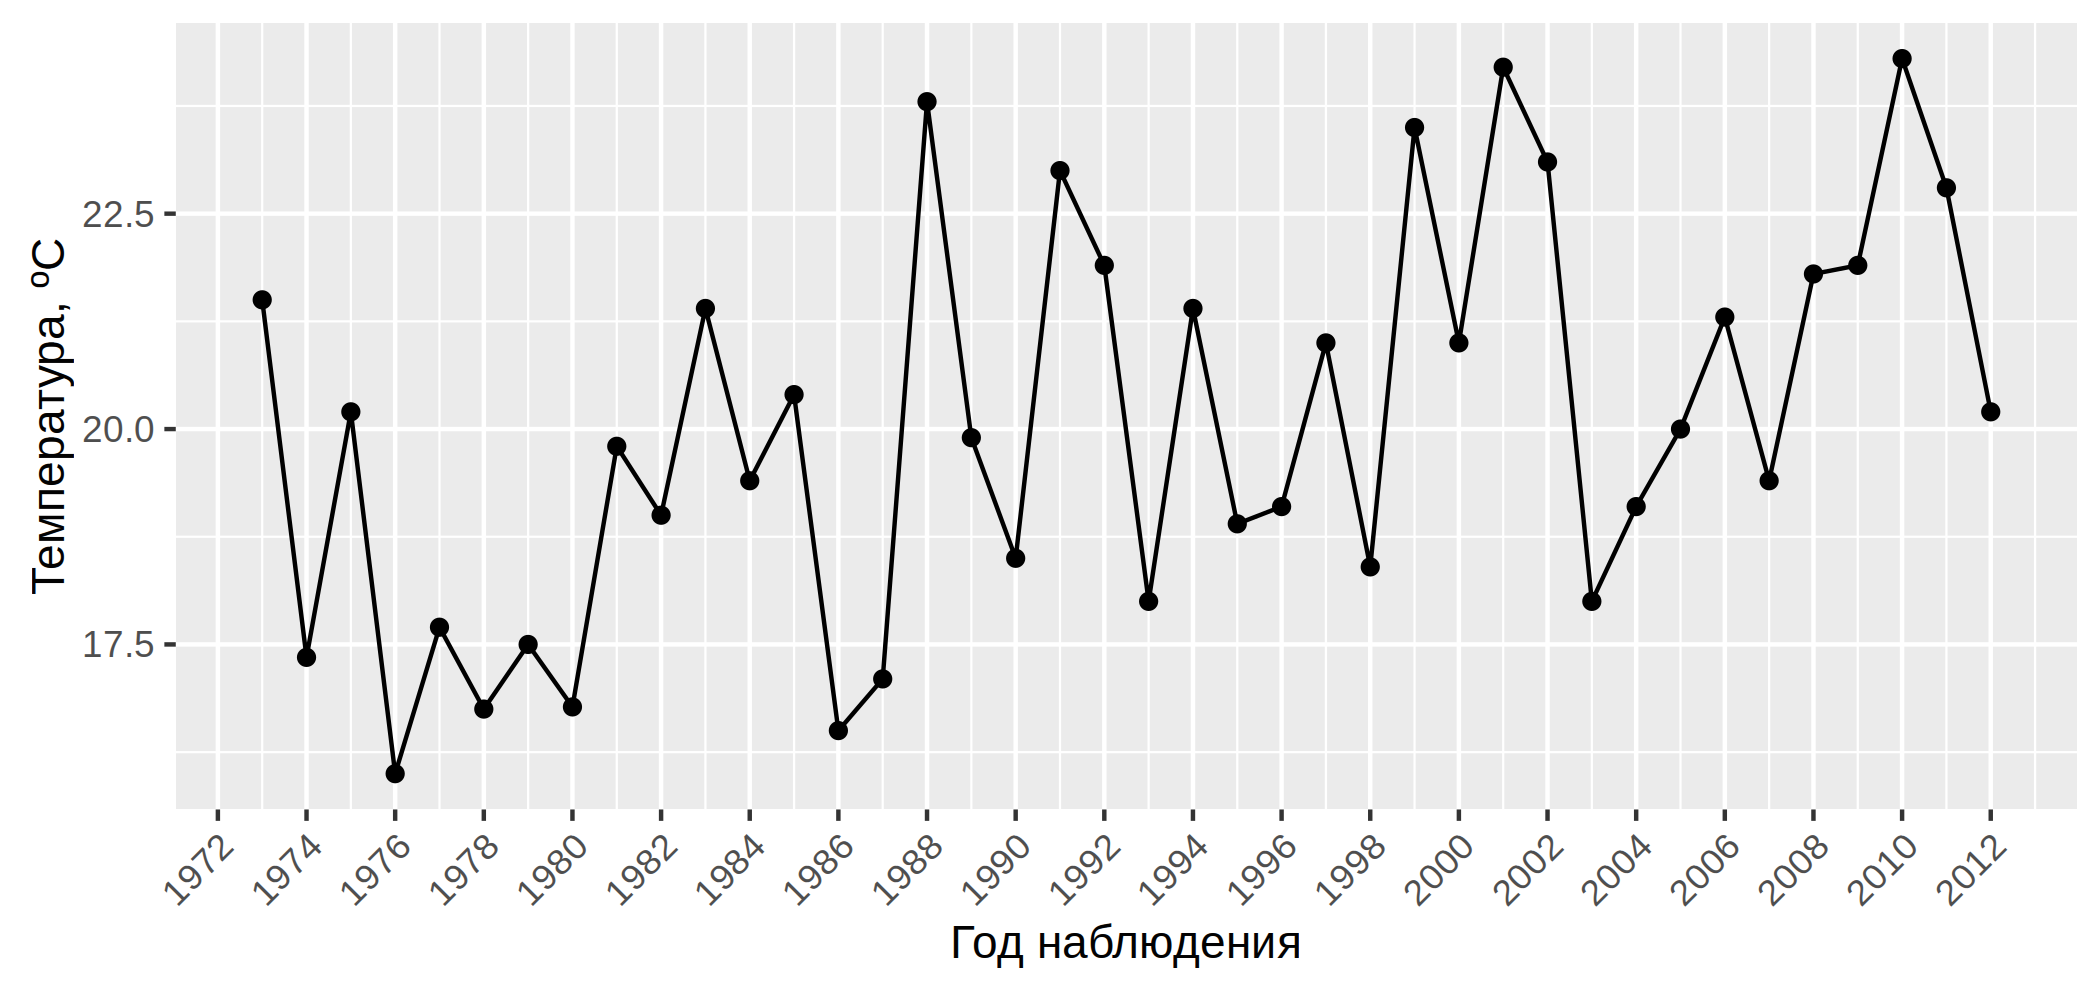
\includegraphics[width=1\linewidth]{../figures/source.png}}
\caption{График исходных данных.}
\label{img:input}
\end{figure}

Следует отметить, что для непосредственного исследования были использованы наблюдения с 1975 по 2009 год. Наблюдения за 2010-2012 годы были намеренно исключены из исследования в целях дальнейшего оценивания результатов анализа и прогнозирования. Заметим, что работа, представленная в параграфах \ref{sec:dstats}--\ref{sec:regr_analysis}, была также проделана и для всей выборки. Так как поведение целой выборки сохранилось в уменьшенной, то, без потери общности, будем считать её исходной.

Начнём исследование временного ряда с вычисления описательных статистик. \textbf{R} предоставляет в пакете \textit{base} различные функции для расчетов базовых статистик. Также, в различных пакетах можно найти другие интересующие функции, как статистические, так и математические. Но в целях удобства, компактности и контроля за функциональностью на основе \cite{Eliseeva1995, Cramer1997} мной был написан модуль \textit{dstats}, представленный в приложении \ref{c:listings} листинге \ref{lst:dstats}. Данный модуль позволяет вычислять все рассмотренные в данной работе описательные статистики. Полученные результаты для исходных данных отображены в таблице \ref{table:dstats}.

% latex table generated in R 3.1.2 by xtable 1.7-4 package
% Fri May 15 14:18:49 2015
\begin{table}[ht]
\centering
\begin{tabular}{rr}
  \hline
 & Значение \\ 
  \hline
Среднее & 19.88 \\ 
  Медиана & 19.80 \\ 
  Нижний квартиль & 18.20 \\ 
  Верхний квартиль & 21.40 \\ 
  Минимум & 16.00 \\ 
  Максимум & 24.20 \\ 
  Размах & 8.20 \\ 
  Квартильный размах & 3.20 \\ 
  Дисперсия & 4.92 \\ 
  Стандартное отклонение & 2.22 \\ 
  Коэффициент вариации & 24.75 \\ 
  Стандартная ошибка & 0.37 \\ 
  Асимметрия & 0.18 \\ 
  Ошибка асимметрии & 0.40 \\ 
  Эксцесс & -0.79 \\ 
  Ошибка эксцесса & 0.78 \\ 
   \hline
\end{tabular}
\caption{Описательные статистики для наблюдаемых температур.} 
\label{table:dstats}
\end{table}


Рассмотрим подробнее некоторые полученные статистики.

Как видно из таблицы, \textit{средняя} температура в июле месяце за период с 1975 по 2009 составляет приблизительно 20ºС. При этом \textit{размах} температур равен 8.2ºC, а \textit{дисперсия} равна $4.91$.

\textit{Стандартное отклонение} оказалось равным приблизительно $2.21$. Полученное значение не велико, а значит можно сказать, что среднее значение хорошо описывает выборку.

\textit{Коэффициент вариации} в нашем случае равен $24.7\%$. Из этого следует, что выборку можно считать однородной, так как полученное значение является меньшим 33\% \cite{Eliseeva1995}.

\textit{Стандартная ошибка среднего значения} равна $0.37$.

\textit{Коэффициент асимметрии} --- мера симметричности распределения. Полученное значение: $0.18$. Данное значение говорит о незначительной правосторонней асимметрии распределения. То есть о том, что выборочное распределение можно считать близким к симметричному \cite{Bulmer1979Principles}.

\textit{Cтандартная ошибка асимметрии} равна $0.40$.

\textit{Коэффициент эксцесса} в рассматриваемом случае равен $-0.85$. Так как коэффициент эксцесса нормального распределения равен $0$, то в данном случае можно говорить о пологости пика распределения выборки по отношению к нормальному распределению \cite{Bulmer1979Principles}.

\textit{Стандартная ошибка коэффициента эксцесса} равна $0.77$.

С помощью тестовых статистик для коэффициента асимметрии и эксцесса \cite[с.85-89]{Cramer1997}, проверим значимость полученных значений для генеральной совокупности. Для этого в модуле \textit{dstats} мной реализованы функции \textit{dstats.test.skew} и \textit{dstats.test.kurtosis}:

Полученная тестовая статистика для коэффициента асимметрии:
\begin{equation*}
	Z_{A_S} = \frac{A_S}{SES} = 0.4648153
\end{equation*}
Данное значение попадает под случай $\vert Z_{A_S} \vert \le 2$, а значит, выборочный коэффициент асимметрии не является значимым. Из чего, в свою очередь, следует, что по нему нельзя судить о коэффициенте асимметрии генеральной совокупности \cite[с.85]{Cramer1997}.

Полученная тестовая статистика для коэффициента эксцесса:
\begin{equation*}
	Z_K = \frac{K}{SEK} = -1.015476.
\end{equation*}
Данное значение попадает под случай $\vert Z_K \vert \le 2$, а значит, в данном случае выборочный коэффициент эксцесса не является значимым и нельзя ничего сказать о коэффициенте эксцесса генеральной совокупности \cite[с.89]{Cramer1997}.

Из полученных результатов следует отметить, что коэффициенты асимметрии и эксцесса, указывают на близость выборочного распределения к нормальному закону. Но при этом, из-за недостаточного объёма выборки, по этим коэффициентам нельзя судить о соответствующих коэффициентах генеральной совокупности.

% section dstats (end)

\section{Исследование статистических данных} % (fold)
\label{sec:analysis}

В \textbf{R} можно найти различные пакеты, позволяющие строить разнообразные гистограммы, диаграммы рассеяния, вероятностные графики, линейные графики, диаграммы диапазонов, размахов, круговые диаграммы, столбчатые диаграммы, последовательные графики и т.д., позволяющие увидеть специфику данных. В процессе работы в контексте \textbf{R} использовались источники \cite{Kabacoff2009R, Teetor2011RCook, Chang2012RGraph}.

С помощью функции пакета \textit{ggplot2} построим гистограмму для отображения вариационного ряда исходных данных \cite{Chang2012RGraph}. Гистограммы позволяют увидеть, как распределены значения переменных по интервалам группировки, то есть как часто переменные принимают значения из различных интервалов. А также, что бывает более важным, повзоляет сделать предположение о разновидности распределения. Для вычисления интервалов разбиения воспользуемся \textit{формулой Стерджеса}. Из \cite{Sturges1926Choice} количество интервалов разбиения рассчитывается по формуле:
\begin{equation}
\label{eq:sturges}
	k = \lceil log_{2}n \rceil + 1 = \lceil log_{2}38 \rceil + 1 = 7.
\end{equation}

Так как по гистограмме можно визуально предположить близость выборочного распределения к нормальному распределению, нанесём на график кривую плотности нормального распределения. Построенная гистограмма отображена на рисунке \ref{img:histogram_fitted}.
\begin{figure}[ht]
	\center{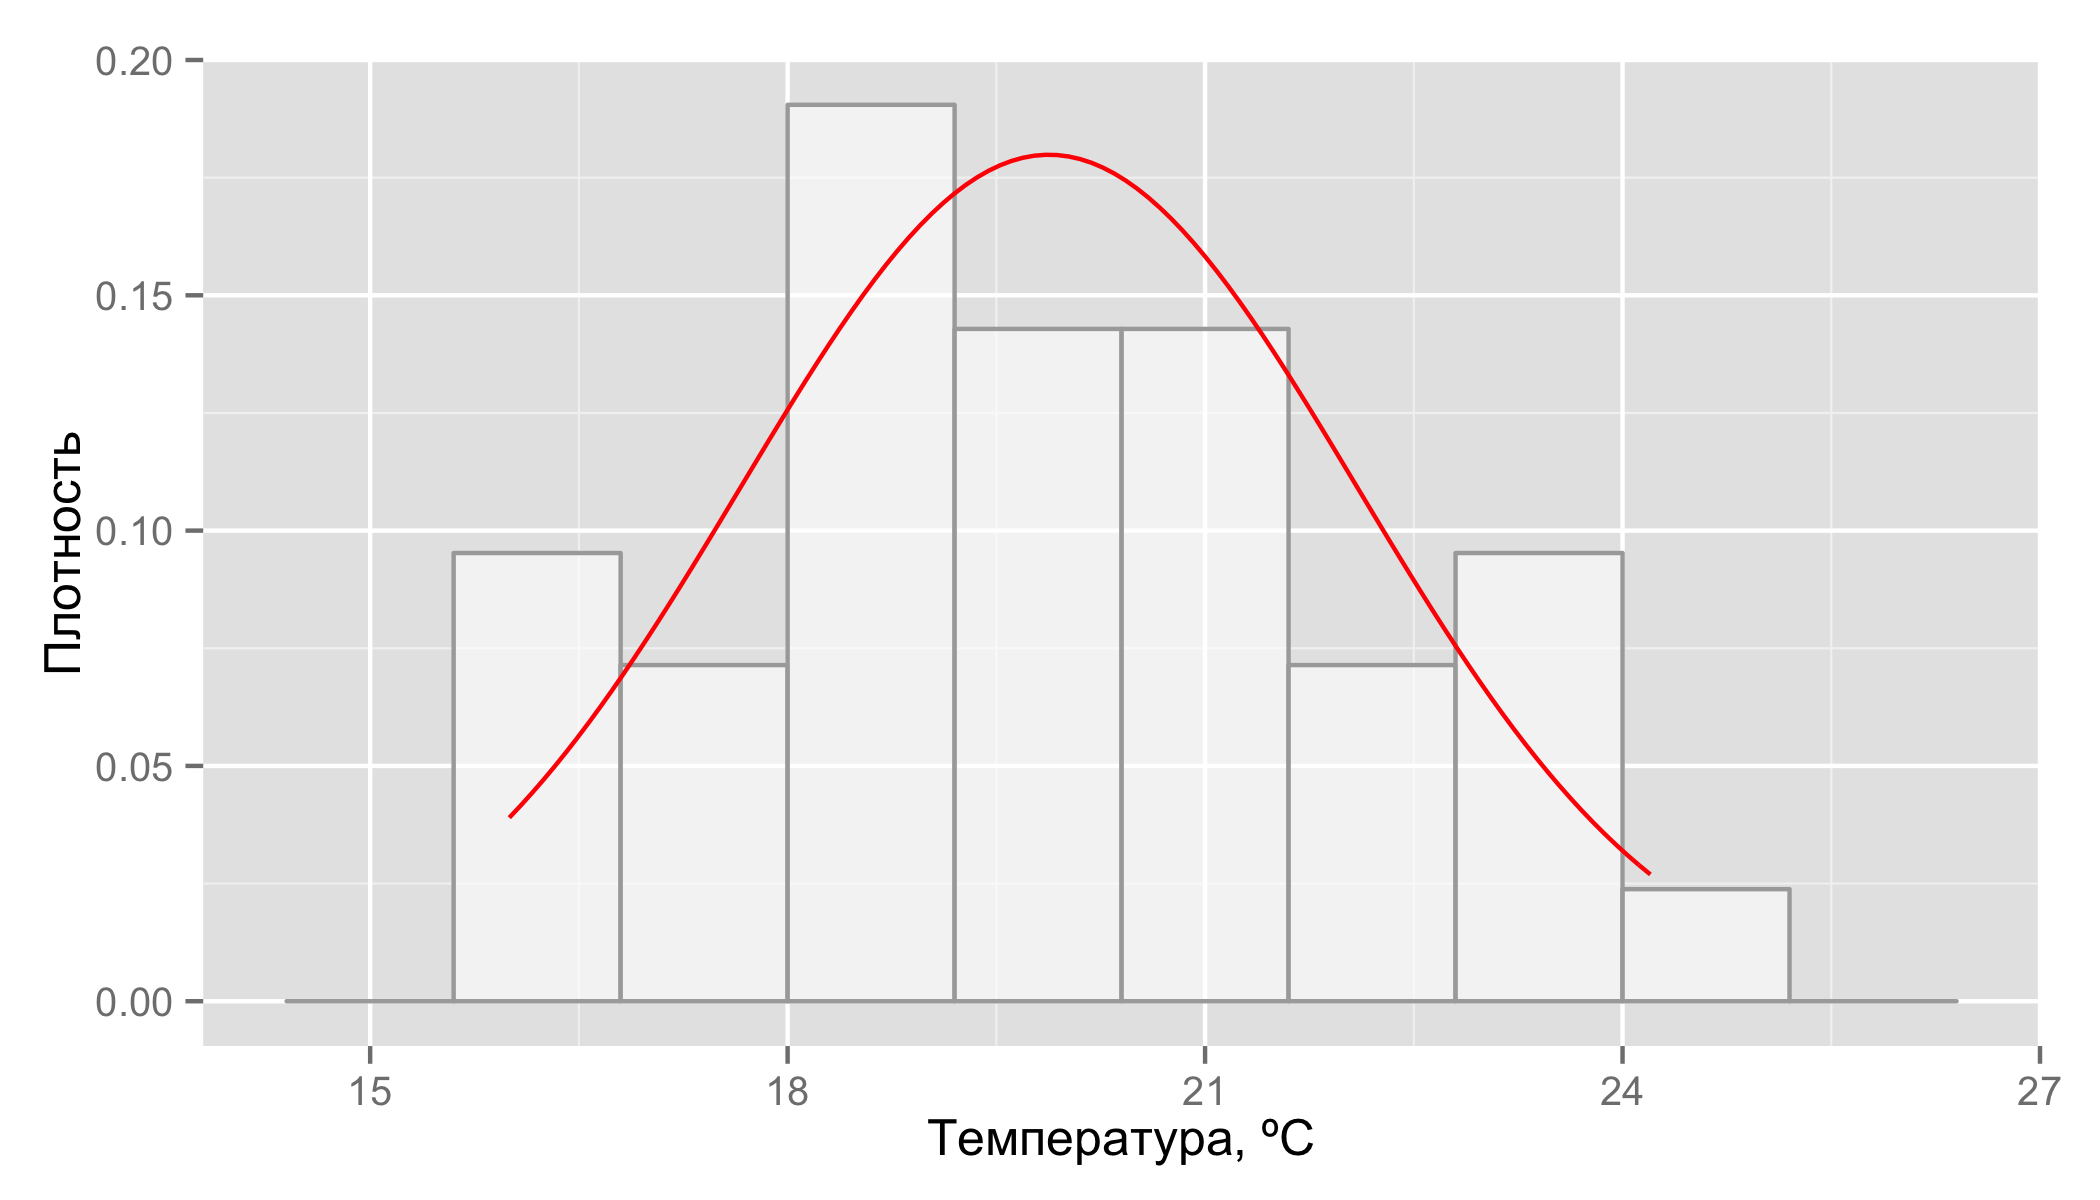
\includegraphics[width=1\linewidth]{../figures/original/histogram.png}}
\caption{Гистограмма наблюдаемых температур с кривой плотности нормального распределения}
\label{img:histogram_fitted}
\end{figure}
Проанализируем эту гистограмму. Во-первых, на ней наглядно представлена близость выборочного распределения к нормальному с параметрами $\mathcal{N}(19.88, 4.91)$. Во-вторых, по этой гистограмме можно подтвердить или опровергнуть результаты, полученные на этапе вычисления описательных статистик в параграфе \ref{sec:dstats}.

Следует отметить согласованность полученных описательных статистик с полученной гистограммой. Во-первых, по коэффициенту асимметрии мы предположили о близости распределения к симметричному. Это подтверждается гистограммой: на ней можно заметить небольшую скошенность вправо, что также согласовывается со знаком коэффициента. Во-вторых, коэффициент эксцесса указывал на пологость пика распределения. Данное заключение подтверждается кривой плотности --- она имеет чуть более растянутую колоколообразную форму.

Другим часто используемым графическим способом проверки характера распределения данных является построение т.н. \textit{графиков квантилей} (\textit{Q-Q plots}, \textit{Quantile-Quantile plots}). На таких графиках изображаются квантили двух распределений --- эмпирического (т.е. построенного по анализируемым данным) и теоретически ожидаемого стандартного нормального распределения. При нормальном распределении проверяемой переменной точки на графике квантилей должны выстраиваться в прямую линию, исходящую под улом 45 градусов из левого нижнего угла графика. Графики квантилей особенно полезны при работе с небольшими по размеру совокупностями, для которых невозможно построить гистограммы, принимающие какую-либо выраженную форму.

В процессе данной работы была написана функция \textit{ggqqp}, с помощью которой построен рисунок \ref{img:qqnorm}.
\begin{figure}[ht]
	\center{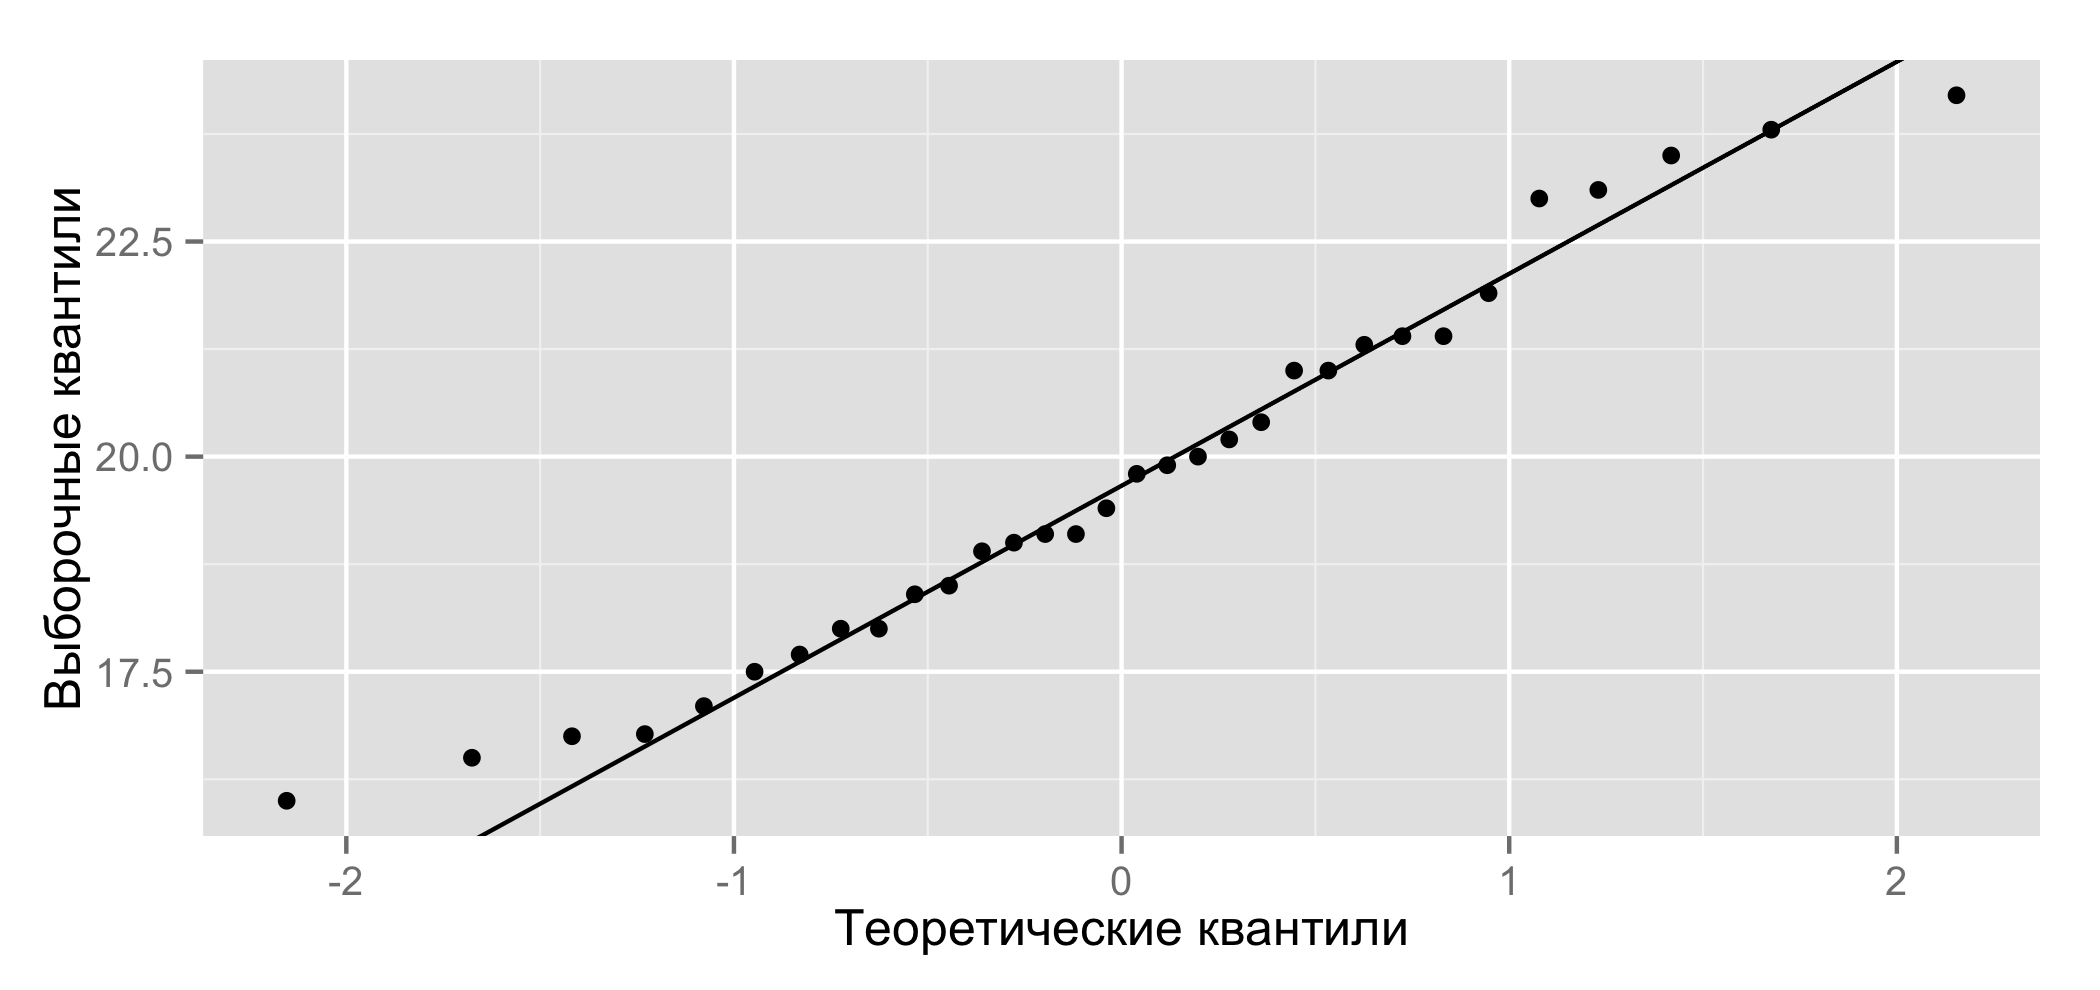
\includegraphics[width=1\linewidth]{../figures/original/quantile.png}}
\caption{График квантилей для наблюдаемых температур}
\label{img:qqnorm}
\end{figure}
На этом графике можно визуально обнаружить аномальное положение наблюдаемых значений по отношению к нормальному распределению. В данном случае отклонения можно наблюдать на концах рассматриваемого промежутка. Остальные значения образуют отчетливую прямую. А значит, подтверждается предположение о нормальности выборочного распределения.

Далее следует проверить полученные результаты с помощью некоторых формальных тестов. Существует целый ряд статистических тестов, специально разработанных для проверки нормальности выборочного распределения. В общем виде проверяемую при помощи этих тестов нулевую гипотезу можно сформулиировать следующим образом: ``Анализируемая выборка происходит из генеральной совокупности, имеющей нормальное распределение''. Если получаемая при помощи того или иного теста вероятность ошибки $P$ оказывается меньше некоторого заранее принятого уровня значимости (например, $0.05$), нулевая гипотеза отклоняется.

В \textbf{R} реализованы практически все имеющиеся тесты на нормальность --- либо в виде стандарных функций, либо в виде функций, входящих в состав отдельных пакетов. Примером базовой функции является \textit{shapiro.test()}, при помощи которой можно выполнить широко используемый \textit{тест Шапиро-Уилка} \cite{Shapiro1972}:
\begin{verbatim} 

	Shapiro-Wilk normality test

data:  data
W = 0.9742, p-value = 0.5685

\end{verbatim}
В полученных результатах $W$ --- статистика Шапиро-Уилка. Вероятность ошибки $p = 0.5685 > 0.05$, а значит нулевая гипотеза не отвергается \cite{Kobzar2006}. Следовательно опровергнуть предположение на основе данного теста нельзя.

Попробуем опровегнуть наше предположение на основе проверки критерия $\chi^2$ Пирсона \cite{Gmurman2003}. Для этого воспользуемся пакетом \textit{nortest} и функцией \textit{pearson.test}:
\begin{verbatim} 

	Pearson chi-square normality test

data:  data
P = 2.8, p-value = 0.8335

\end{verbatim}
В полученных результатах $P$ --- статистика $\chi^2$ Пирсона. Вероятность ошибки $p = 0.8335 > 0.05$, а значит нулевая гипотеза не отвергается. Следовательно опровергнуть предположение о нормальности на основе данного теста также нельзя. Проверим критерий: примем уровень значимости $\alpha = 0.05$, тогда из таблицы распределения $\chi^2$ найдём критическое значение критерия $P_{\textrm{кр}}(\alpha, k) = 43.8$. Отсюда следует, что

\begin{equation*}
	P < P_{\textrm{кр}}.
\end{equation*}

А значит, нулевую гипотезу при уровне значимости $\alpha = 0.05$ не отвергаем и подтверждаем сделанный вывод на основании вычисленной вероятности ошибки. 

Воспользуемся для тех же целей критерием Колмогорова--Смирнова \cite{Mikulik2002}. Как в предыдущем случае воспользуемся представленной в пакете \textit{nortest} функцией \textit{ks.test}:
\begin{verbatim} 

	Two-sample Kolmogorov-Smirnov test

data:  data and nsample
D = 0.0706, p-value = 0.995
alternative hypothesis: two-sided

\end{verbatim}
Вероятность ошибки $p > 0.05$, а значит нулевую гипотезу отвергнуть нельзя. Следовательно опровергнуть предположение о нормальности, как и предыдущих случаях, также нельзя. Проверим критерий: примем так же уровень значимости $\alpha = 0.05$, тогда критическое значение $D_{\textrm{кр}}(\alpha) = 1.358$. Следовательно,
\begin{equation*}
	D < D_{\textrm{кр}}(\alpha),
\end{equation*}
и подтверждаем сделанные ранее заключения: нельзя отвергнуть нулевую гипотезу о нормальности выборочного распределения.

На данном этапе по полученным ранее результатам возникли подозрения о выбросах в исходной выборке. Выявление таких аномальных значений важно, так как их наличие, как правило, сильно влияет на всю выборку, в частности, на коэффициент корреляции. Проверим наличие выбросов с помощью статистических критериев. Для этих целей воспользуемся критерием Граббса \cite{Grubbs1950Sample}. Данный основан на предположении о нормальности исходных данных. То есть, перед применением данного критерия необходимо убедиться, что данные могут быть в разумных пределах аппроксимированы нормальным распределением \cite{grubbs}. Поскольку ранее высказано предположение о нормальности, воспользуемся им для определения наличия выбросов.

Полученные результаты проверки критерия Граббса:
\begin{verbatim} 

	Grubbs test for one outlier

data:  research.data$temperature
G = 1.9487, U = 0.8850, p-value = 0.8103
alternative hypothesis: highest value 24.2 is an outlier

\end{verbatim}
Данный результат ($p\textrm{-value} = 1$) однозначно говорит нам о том, что следует отклонить альтернативную гипотезу $H_{1}$ и принять гипотезу $H_{0}$. Другими словами, это говорит о том, что в исходной выборке нету выбросов. А значит выборка однородна. Значит, наши подозрения о выбросах не подтвердились проверкой критерия.

В соответствии с результатами проверки критериев и на основе построенных гистограммы и графика квантилей, можно сделать заключение о том, что распределение температуры воды озера Баторино в июле 1975--2009 годов является близким к нормальному закону распределения с параметрами $\mathcal{N}(19.88, 4.91)$. Что подтверждается коэффициентами асимметрии и эксцесса из таблицы \ref{table:dstats}, а также результатами, полученными мной при исследовании в пакете \textbf{STATISTICA}. Следует также отметить, что такие же результаты были получены и для всей выборки.

% section analysis (end)

\section{Корреляционный анализ} % (fold)
\label{sec:corr_analysis}

Исследуем теперь зависимость температуры воды от времени, построив диаграмму рассеяния и вычислив коэффициент корреляции соответствующих переменных.

Диаграммы рассеяния используются для визуального исследования зависимости между двумя переменными. Если переменные сильно связаны, то множество точек данных принимает определённую форму. С помощью таких диаграмм можно наглядно изучить знак коэффициента корреляции. Если точки на диаграмме расположены хаотически, то это говорит о независимости рассматриваемых переменных. Если с ростом переменной $t$ возрастает переменная $x$ то имеет место положительная корреляция. Если же с ростом переменной $t$ переменная $x$ убывает, то это указывает на отрицательную корреляцию. 
\begin{figure}[ht]
	\center{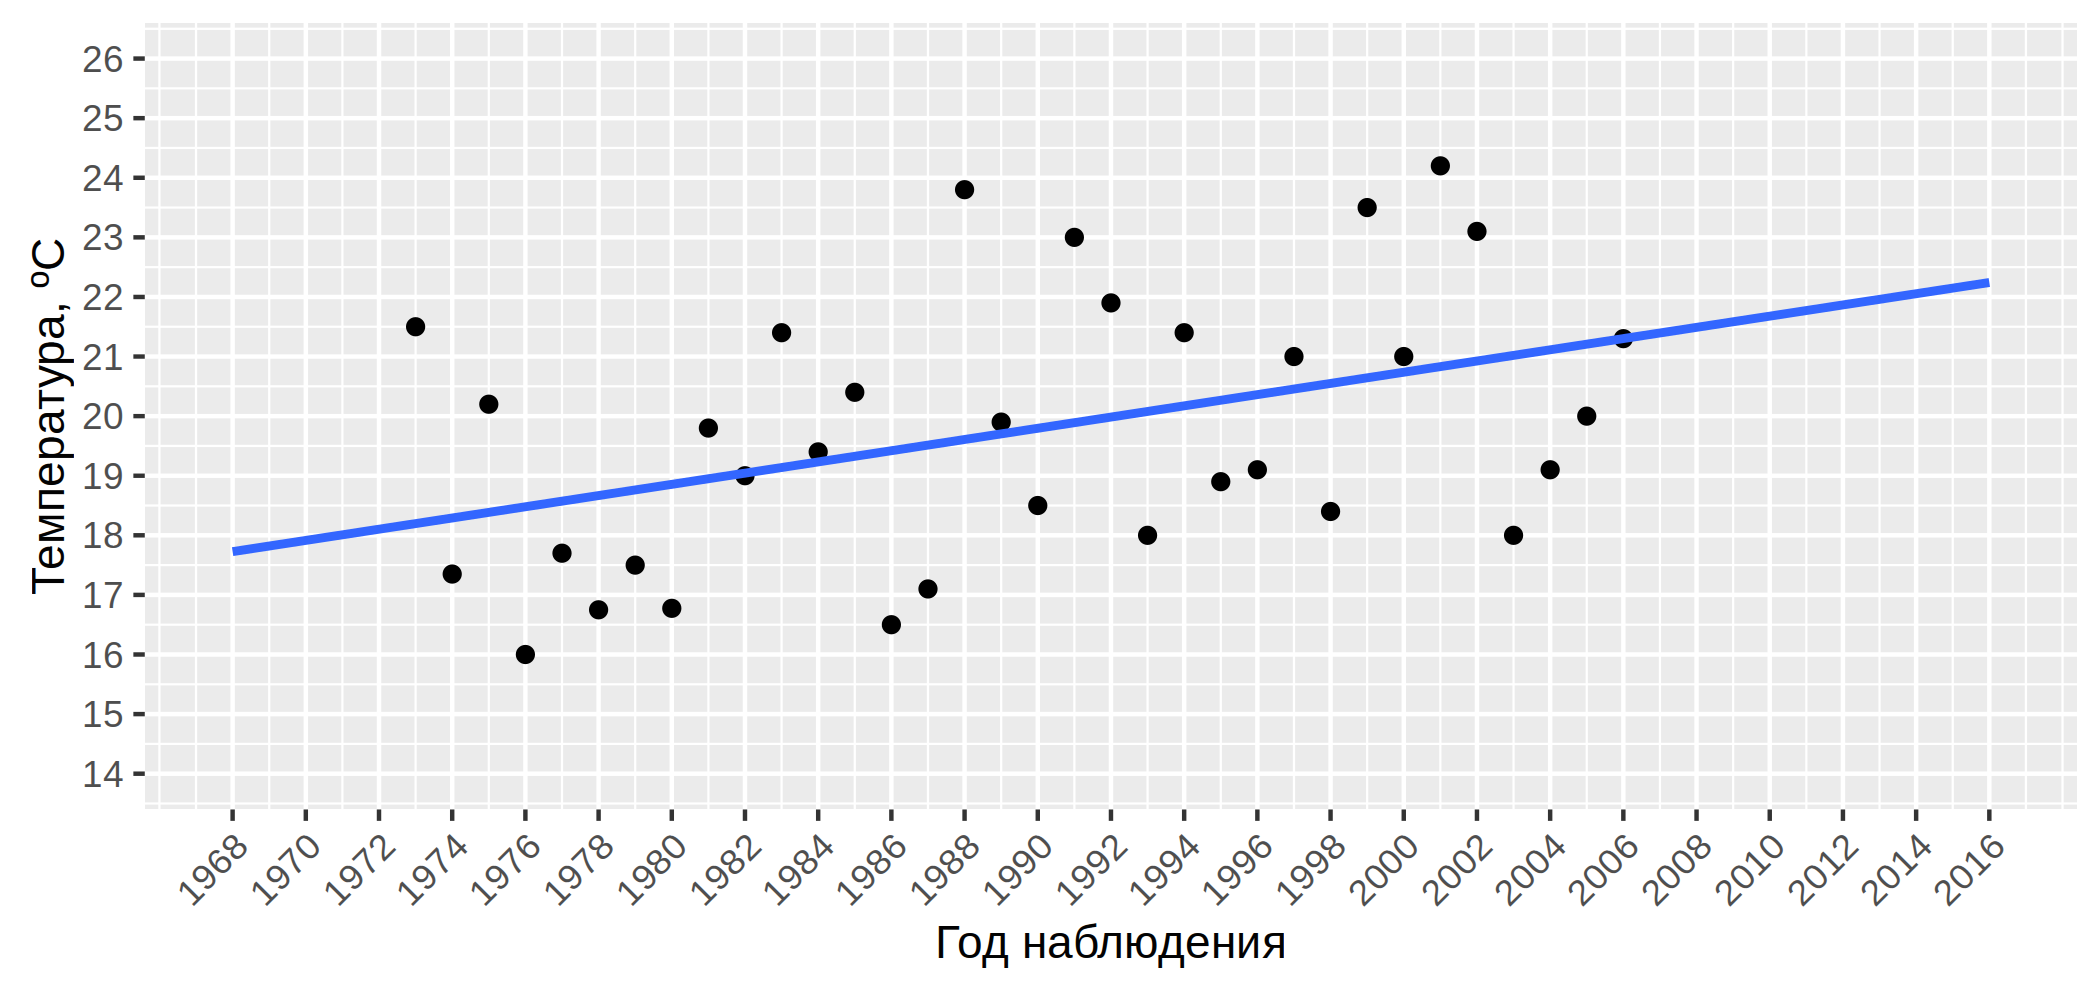
\includegraphics[width=1\linewidth]{../figures/original/scatterplot.png}}
\caption{Диаграмма рассеяния}
\label{img:scatterplot}
\end{figure}

Из рисунка \ref{img:scatterplot} видно, что точки образуют своеобразное <<облако>>, ориентированное по диагонали вверх, то есть присутствует некая зависимость между рассмтриваемыми переменными. Также, данная диаграмма наглядно показывает силу этой зависимости: так как точки не образуют чёткой формы, а разбросаны относительно диагонали, то можно говорить о наличии умеренной корреляции. То есть, нельзя сказать, что зависимость сильная, но и нельзя сказать, что связь между переменными отсутствует.

Проверим полученные результаты подробнее. Для начала построим корреляционную матрицу.
% latex table generated in R 3.1.2 by xtable 1.7-4 package
% Tue Feb 24 18:11:02 2015
\begin{table}[ht]
\centering
\begin{tabular}{rrr}
  \hline
 & Temperature & Date \\ 
  \hline
Temperature & 1.00 & 0.47 \\ 
  Date & 0.47 & 1.00 \\ 
   \hline
\end{tabular}
\caption{Корреляционная матрица.} 
\label{table:cmatrix}
\end{table}

Как видно из таблицы \ref{table:cmatrix}, коэффициент корреляции $r_{xt} = 0.47$. Этим подтверждаются наши выводы из диаграмм рассеяния и концентрации о положительной корреляции, поскольку полученный коэффициент корреляции является положительным и присутствует умеренная зависимость: $r_{xt} \approx 0.5$.

Оценим значимость полученного выборочного коэффициента корреляции с помощью возможностей пакета \textbf{R} и описанного ранее в параграфе критерия значимости. Вычислим:
\begin{equation*}
	T_{\textrm{набл}} = \frac{r_{xt} \sqrt{n - 2}}{\sqrt{1 - r_{xt}^2}} \approx 3.05885.
\end{equation*}
Рассмотрим уровень значимости $\alpha = 0.05$. Число степеней свободы $k = n - 2 = 36$. Тогда из таблицы критических точек распределения Стьюдента $t_\textrm{кр}(\alpha, k) \approx 2.03$. Следовательно,
\begin{equation*}
	T_{\textrm{набл}} > t_\textrm{кр}(\alpha, k).
\end{equation*}
Значит нулевую гипотезу о равенстве нулю коэффициента корреляции генеральной совокупности следует отклонить \cite{Eliseeva1995}.

Пакет \textbf{R} предоставляет с помощью функции \textit{cor.test} различные методы для проверки значимости выборочного коэффициента корреляции. Воспользуемся проверкой теста методом Пирсона:
\begin{verbatim} 

	Pearson's product-moment correlation

data:  research.data$temperature and c(1:kObservationNum)
t = 3.0471, df = 33, p-value = 0.004523
alternative hypothesis: true correlation is not equal to 0
95 percent confidence interval:
 0.1603947 0.6935396
sample estimates:
      cor 
0.4685944 

\end{verbatim}
Как видно из полученных результатов $p-value < 0.05$, следовательно это говорит, о том, что необходимо отвегнуть гипотезу $H_0: r = 0$.

Значит, нулевую гипотезу о равенстве нулю коэффициента корреляции генеральной совокупности отвергаем и подтверждаем правильность полученных с помощью \textbf{R} результатов. Другими словами, выборочный коэффициент значимо отличается от нуля, т.е. температура воды и время при уровне значимости $\alpha = 0.05$ имеют зависимость.

Следует также отметить, что аналогичный анализ, проведённый в пакете STATISTICA, аналогичным образом выявил зависимость между температурой воды и временем.

Следовательно, в рассматриваемом случае можно говорить о присутствии значимой зависимости между температурой воды в озере Баторино и временем.

% section corr_analysis (end)

\section{Регрессионный анализ} % (fold)
\label{sec:regr_analysis}

Для введения последующих понятий анализа временных рядов воспользуемся \cite{Eddows1997}.

В отличие от анализа случайных выборок, анализ временных рядов основывается на предположении, что последовательные значения в файле данных наблюдаются через равные промежутки времени.

Большинство методов исследования временных рядов включает различные способы фильтрации шума, выделения сезонной и циклической составляющих, позволяющие увидеть регулярную составляющую более отчётливо.

Во временных рядах выделяют три составляющие:
\begin{enumerate}
	\item \textit{Тренд (тенденция развития) ($T$)} --- эволюционная составляющая, которая характеризует общее направление развития изучаемого явления и связанна с действием долговременных факторов развития.
	\item \textit{Циклические ($K$), сезонные ($S$) колебания} --- это составляющие, которые проявляются как отклонения от основной тенденции развития изучаемого явления, и связанны с действие краткосрочных, систематических факторов развития. Циклические колебания состоят в том, что значения признака в течение какого-то времени возрастают, достигают определённого максимума, затем убывают, достигают определённого минимума, вновь возрастают до прежних значений и т.д. Эту составляющую можно выявить только по данным за длительные промежутки времени, например, в 10, 15 или 20 лет. Сезонные колебания --- это колебания, периодически повторяющиеся в некоторое определённое время каждого года, месяца, недели, дня. Эти изменения отчётливо наблюдаются на графиках рядов динамики, содержащих данные за период не менее одного года.
	\item \textit{Нерегулярная случайная составляющая (ошибка) ($E$)}, являющаяся результатом действия второстепенных факторов развития.
\end{enumerate}
Первые два типа компонент представляют собой детерминированные составляющие. Случайная составляющая образована в результате суперпозиции некоторого числа внешних факторов.

По типу взаимосвязи вышеперечисленных составляющих ряда динамики можно построить следующие модели временных рядов ($X$):

\begin{itemize}
	\item Аддитивная модель: $X = T + K + S + E$;
	\item Мультипликативная модель: $X = T \times K \times S \times E$.
\end{itemize}
Аддитивной модели свойственно то, что характер циклических и сезонных колебаний остаётся постоянным.

В мультипликативной модели характер циклических и сезонных колебаний остаётся постоянным только по отношению к тренду (т.е. значения этих составляющих увеличиваются с возрастанием значений тренда).

По причине того, что в данном случае мы рассматриваем один месяц в году на протяжении длительного периода, будем считать, что в нашем временном ряде циклическая и сезонная составляющие отсутствуют. Построим график временного ряда.

\begin{figure}[ht]
	\center{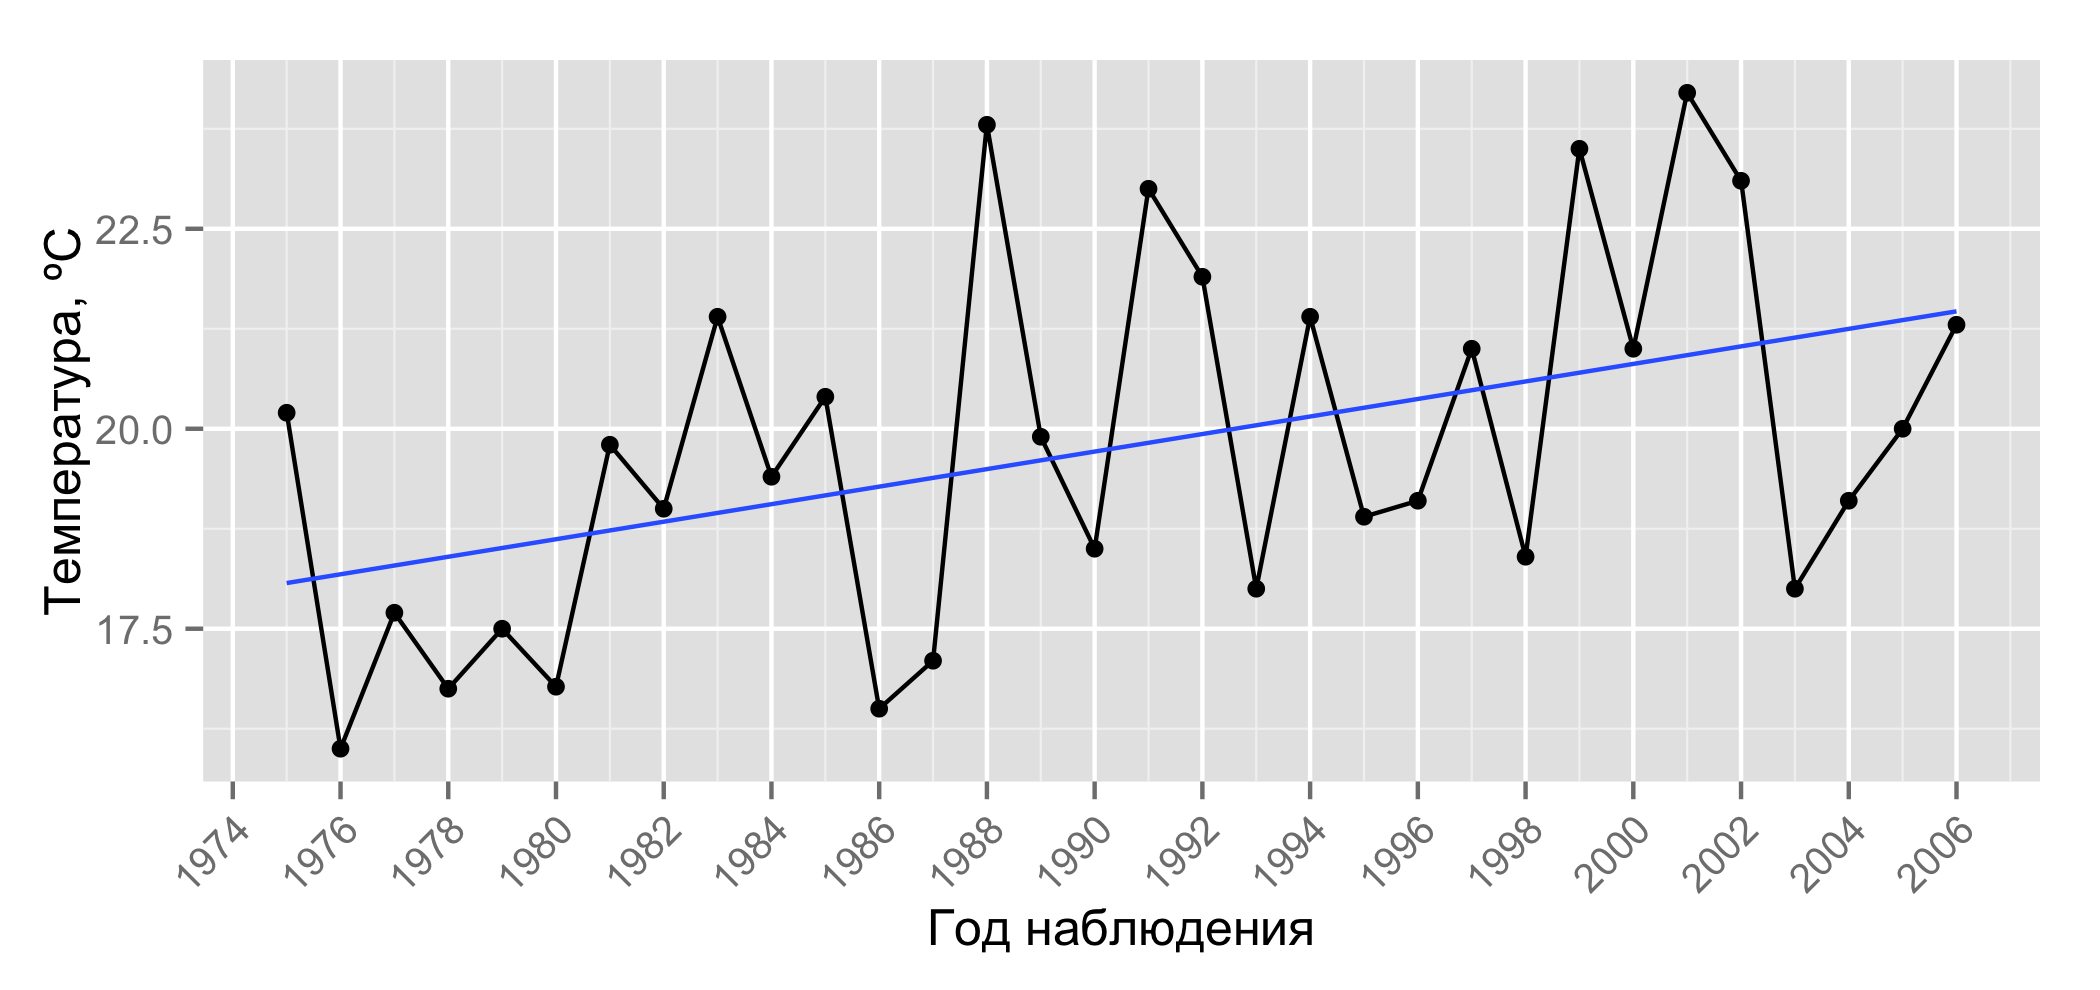
\includegraphics[width=1\linewidth]{../figures/original/time-series.png}}
\caption{График временного ряда с линией регрессии}
\label{img:ts_regr}
\end{figure}

На полученном графике можно заметить явно выраженный линейный рост значений со временем --- он проиллюстрирован на графике прямой. Эта составляющая нашего временного ряда --- тренд. Из этого следует, что уравнение тренда имеет вид:
\begin{equation*}
	x = at + b.
\end{equation*}

Продолжая рассуждение, как наблюдение из графика, можно отметить, что не происходит увеличения амплитуды колебаний с течением времени. А значит, данная модель является аддитивной. Из всего вышесказанного можно заключить, что модель исходного временного ряда имеет вид:
\begin{equation*}
	X = T + E.
\end{equation*}

В \textbf{R} реализованы функции, позволяющие подгонять линейные модели к исследуемым данным \cite{Shumway2006Time}. Одной из таких функций является \textit{lm(Fitting Linear Model)} \cite[c.178]{Kabacoff2009R}. Она позволяет получить коэффициенты линии регрессии(тренд), остатки после удаления тренда. Коэффицинты, полученные с помощью данной функции представлены в \eqref{eq:regr_coeff}.
\begin{equation}
\label{eq:regr_coeff}
	a = 0.1014, \quad b = 18.0521.
\end{equation}
Следует отметить, что в пакете \textbf{STATISTICA} похожая процедура была проведена для всей выборки с помощью инструмента \textit{Trend Subtract}, результаты которой согласуется с полученными в \textbf{R} коэффициентами. Отметим также, что эти результаты подтверждаются вычислениями в \textbf{Excel}.

Таким образом получена линейная модель, описывающая тенденцию развития:
\begin{equation}
\label{eq:regr}
	x = at + b = 0.1014t + 18.0521
\end{equation}

На основе полученной линейной модели \eqref{eq:regr}, построим ряд остатков(приложение \ref{c:app_results}, таблица \ref{table:residuals}), удалив тренд из исходного ряда. Полученный ряд представлен на рисунке \ref{img:ts_detrended}.
\begin{figure}[ht]
	\center{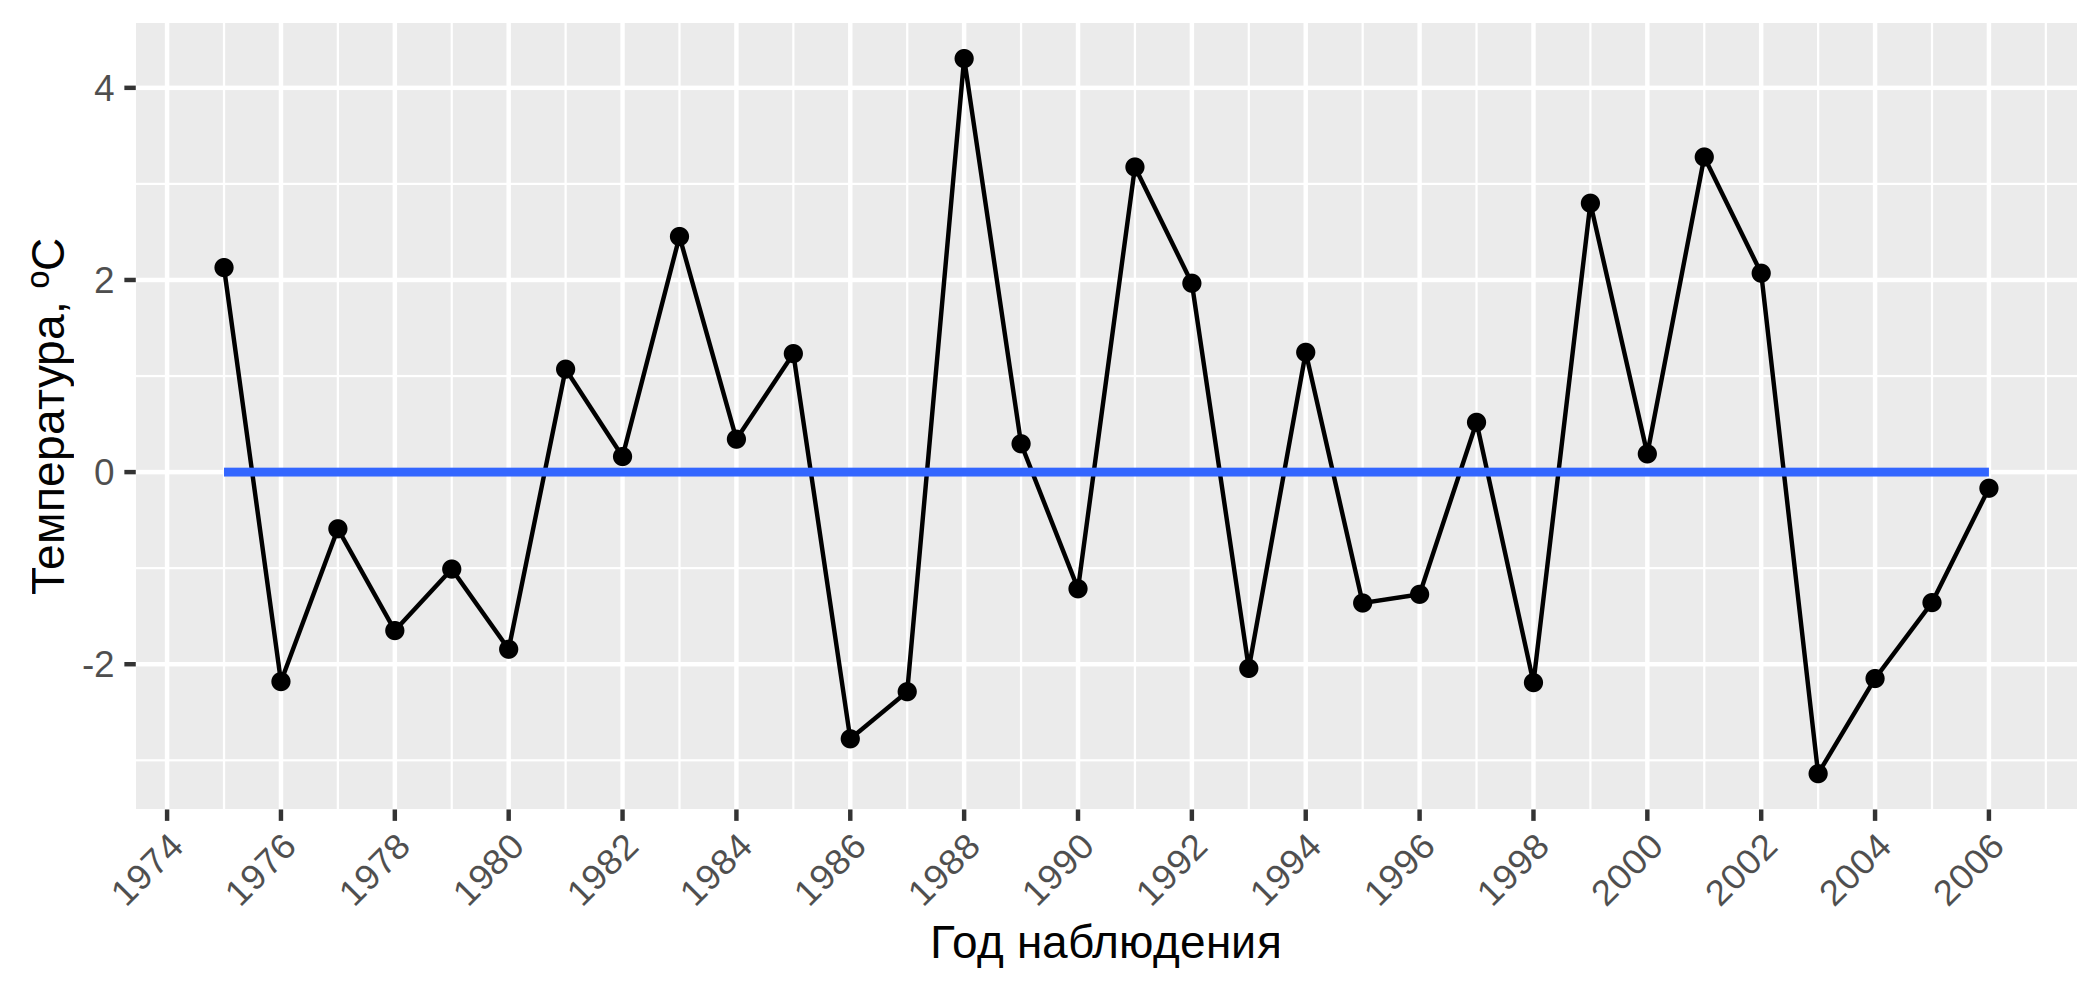
\includegraphics[width=1\linewidth]{../figures/residual/time-series.png}}
\caption{График ряда остатков}
\label{img:ts_detrended}
\end{figure}

Проведём анализ полученной регрессионной модели. Для этого проверим значимость полученных коэффициентов регрессии и оценим адекватность регрессионной модели.

Рассчитаем вспомогательные величины, воспользовавшись \cite{Eddows1997}. Дисперсия отклонения
\begin{equation*}
	\sigma_{\varepsilon}^2 \approx 3.823,
\end{equation*}
стандартные случайные погрешности параметров $a, b$:
\begin{equation*}
	\sigma_{a} \approx 0.029, \quad \sigma_{b} \approx 0.356.
\end{equation*}

Воспользуемся критерием значимости коэффициентов линейной регрессии \cite{Eliseeva1995}. Примем уровень значимости $\alpha = 0.05$, тогда
\begin{equation*}
	T_{a} = 38.2, \quad T_{b} = 50.5.
\end{equation*}

Число степеней свободы $k = 36$, $t_{\textrm{кр}}(k, \alpha) = 2.028$.

\begin{itemize}
	\item $\vert T_{a} \vert > t_{\textrm{кр}}$ $\Rightarrow$ коэффициент $a$ значим.
	\item $\vert T_{b} \vert > t_{\textrm{кр}}$ $\Rightarrow$ коэффициент $b$ значим.
\end{itemize}
Следовательно, при уровне значимости $\alpha = 0.05$, коэффициенты линейной регрессии являются значимыми.

Оценим адекватность полученной регрессионной модели. Дисперсия модели:
\begin{equation*}
	\overline{\sigma^2} \approx 1.44.
\end{equation*}

Остаточная дисперсия:
\begin{equation*}
	\overline{D} \approx 3.7.
\end{equation*}

Воспользуемся F-критерием Фишера. Пусть уровень значимости $\alpha = 0.05$,
\begin{equation*}
	F_{\textrm{крит}} \approx 14.01,
\end{equation*}
при степенях свободы $v_1 = 1, v_2 = 36, F_{\textrm{табл}}(v_1, v_2, \alpha) = 4.11$.

\begin{equation*}
	F_{\textrm{крит}} > F_{\textrm{табл}}.
\end{equation*}
Следовательно, при уровне значимости $\alpha = 0.05$, регрессионная модель является адекватной.

Рассчитаем коэффициент детерминации:
\begin{equation*}
	\eta_{x(t)}^2 \approx 0.275.
\end{equation*}

Проверим отклонение от линейности: $\eta_{x(t)}^2 - r_{xt}^{2} \approx 0.0044 \le 0.1$. Следовательно отклонение от линейности незначительно. Но при этом коэффициент детерминации оказался не достаточно высоким($<0.7$), это говорит о том, что построенная регрессионная модель не описывает в достаточной мере поведение временного ряда. Это, в свою очередь, может значить, что изменение температуры зависит не только от времени, но ещё и от каких-то других, неучтённых, факторов.

Тем не менее, попробуем построить прогноз по полученной модели. Вычисленые прогнозные значения на 2010-2012 годы: $21.87$ – 2010 год, $21.98$ – 2011 год, $22.08$ – 2012 год. Фактические данные на этот период: $24.3$, $22.8$, $20.2$ соответственно. Имеющееся отклонение прогнозов от реальных данных еще раз подтверждает, что построенная модель временного ряда обладает невысокой точностью.

Проанализируем временной ряд остатков. Для этого проверим свойства, которым должна удовлетворять нерегулярная составляющая $\varepsilon$:
\begin{enumerate}
	\item $E(\varepsilon) = 0$.
	\item Дисперсия $\varepsilon$ постоянна для всех значений.
	\item Остатки независимы и нормально распределены.
\end{enumerate}
Вычислим описательные статистики для остатков. Полученные результаты проследим по таблице \ref{table:residuals_dstats}.
% latex table generated in R 3.1.2 by xtable 1.7-4 package
% Mon Mar  2 02:32:46 2015
\begin{table}[ht]
\centering
\begin{tabular}{rr}
  \hline
 & Значение \\ 
  \hline
Среднее & -0.00 \\ 
  Медиана & 0.14 \\ 
  Нижний квартиль & -1.80 \\ 
  Верхний квартиль & 1.28 \\ 
  Минимум & -2.99 \\ 
  Максимум & 4.33 \\ 
  Размах & 7.32 \\ 
  Квартильный размах & 3.07 \\ 
  Дисперсия & 3.84 \\ 
  Стандартное отклонение & 1.96 \\ 
  Коэффициент вариации & 0.00 \\ 
  Стандартная ошибка & 0.33 \\ 
  Асимметрия & 0.42 \\ 
  Ошибка асимметрии & 0.40 \\ 
  Эксцесс & -0.77 \\ 
  Ошибка эксцесса & 0.78 \\ 
   \hline
\end{tabular}
\caption{Описательные статистики остатков} 
\label{table:residuals_dstats}
\end{table}


Как видно из таблицы \ref{table:residuals_dstats}, среднее значение равно нулю. При этом коэффициенты асимметрии($A_S \approx 0.37$) и эксцесса($K \approx -0.87$) указывают на отклонение распределения остатков от нормального закона.

Построим гистограмму и график квантилей для проверки последних заключений.
\begin{figure}[ht]
	\center{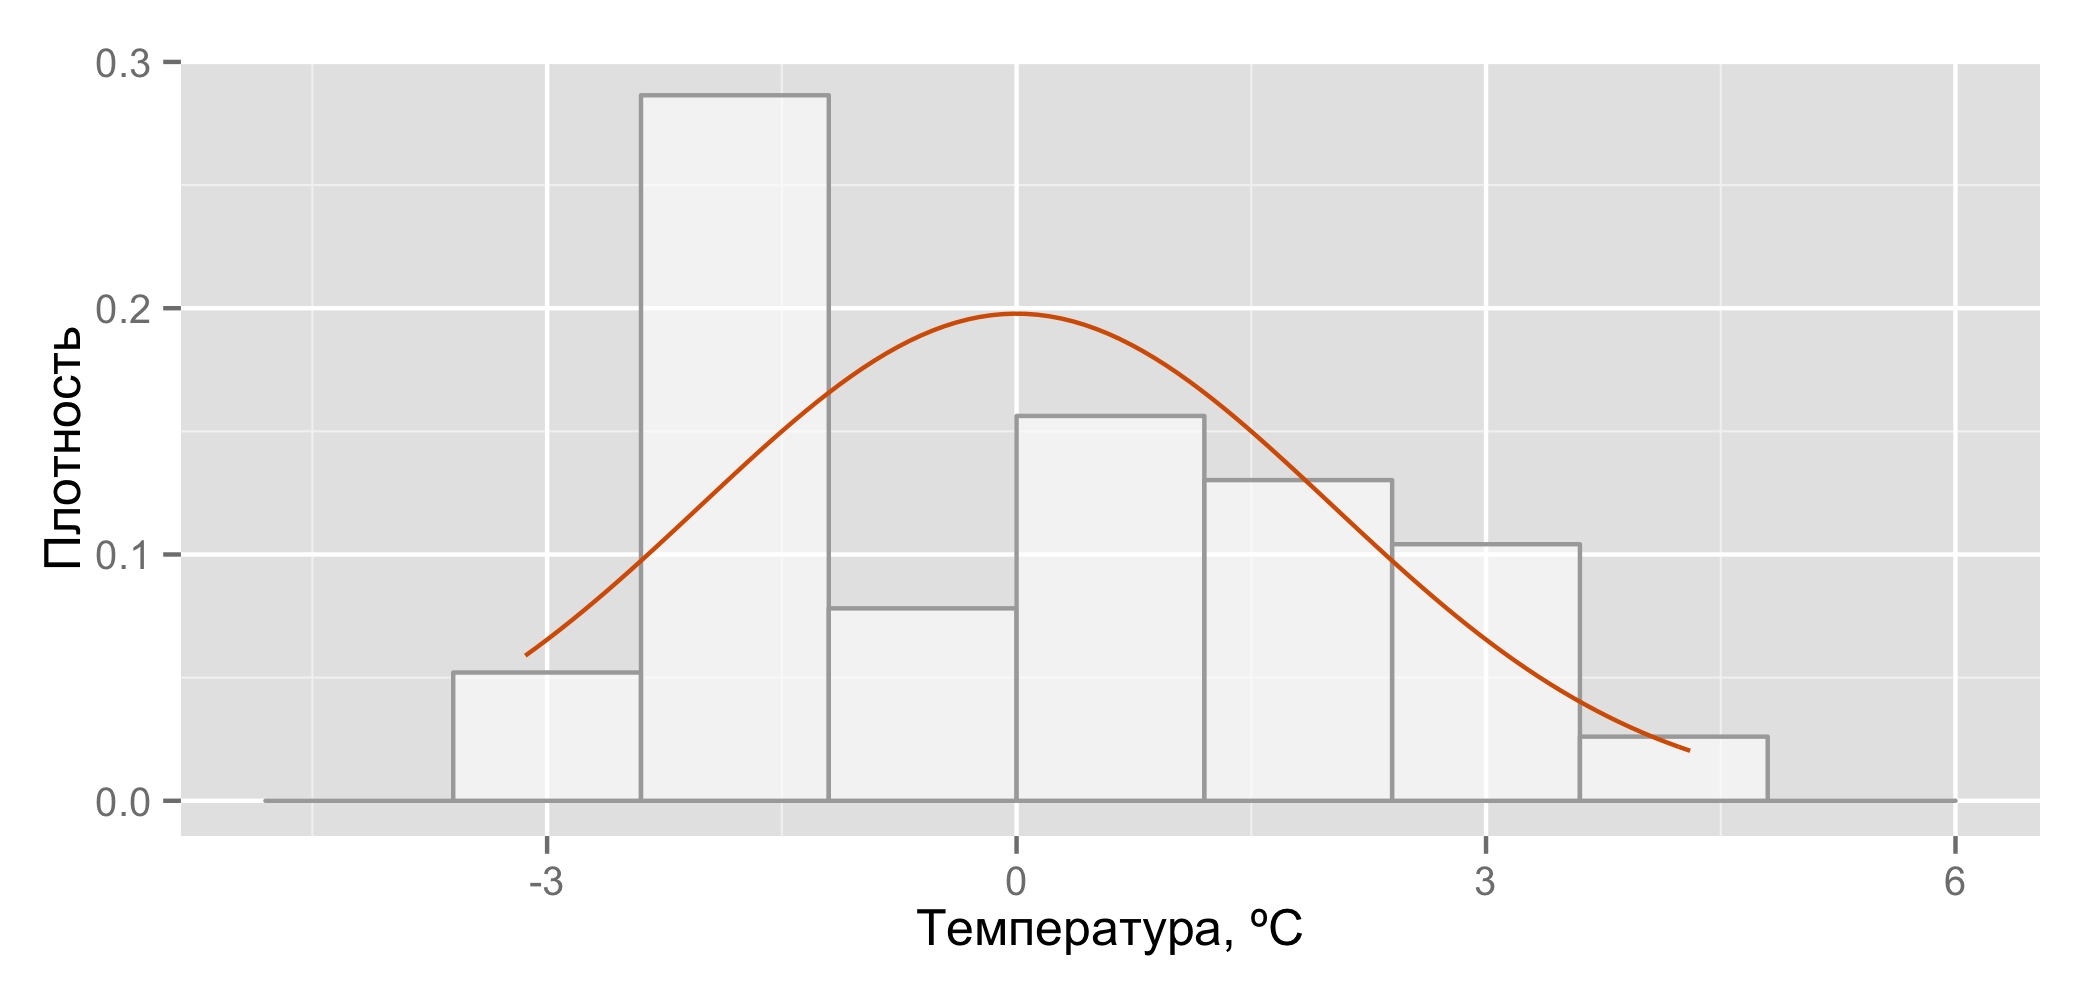
\includegraphics[width=1\linewidth]{../figures/residual/histogram.png}}
\caption{Гистограмма остатков с кривой плотности нормального распределения}
\label{img:resid_hist}
\end{figure}
Гистограмма наглядно демонстрирует полученные в таблице \ref{table:residuals_dstats} коэффициенты асимметрии и эксцесса.

Для проверки нормальности построим график квантилей.
\begin{figure}[ht]
	\center{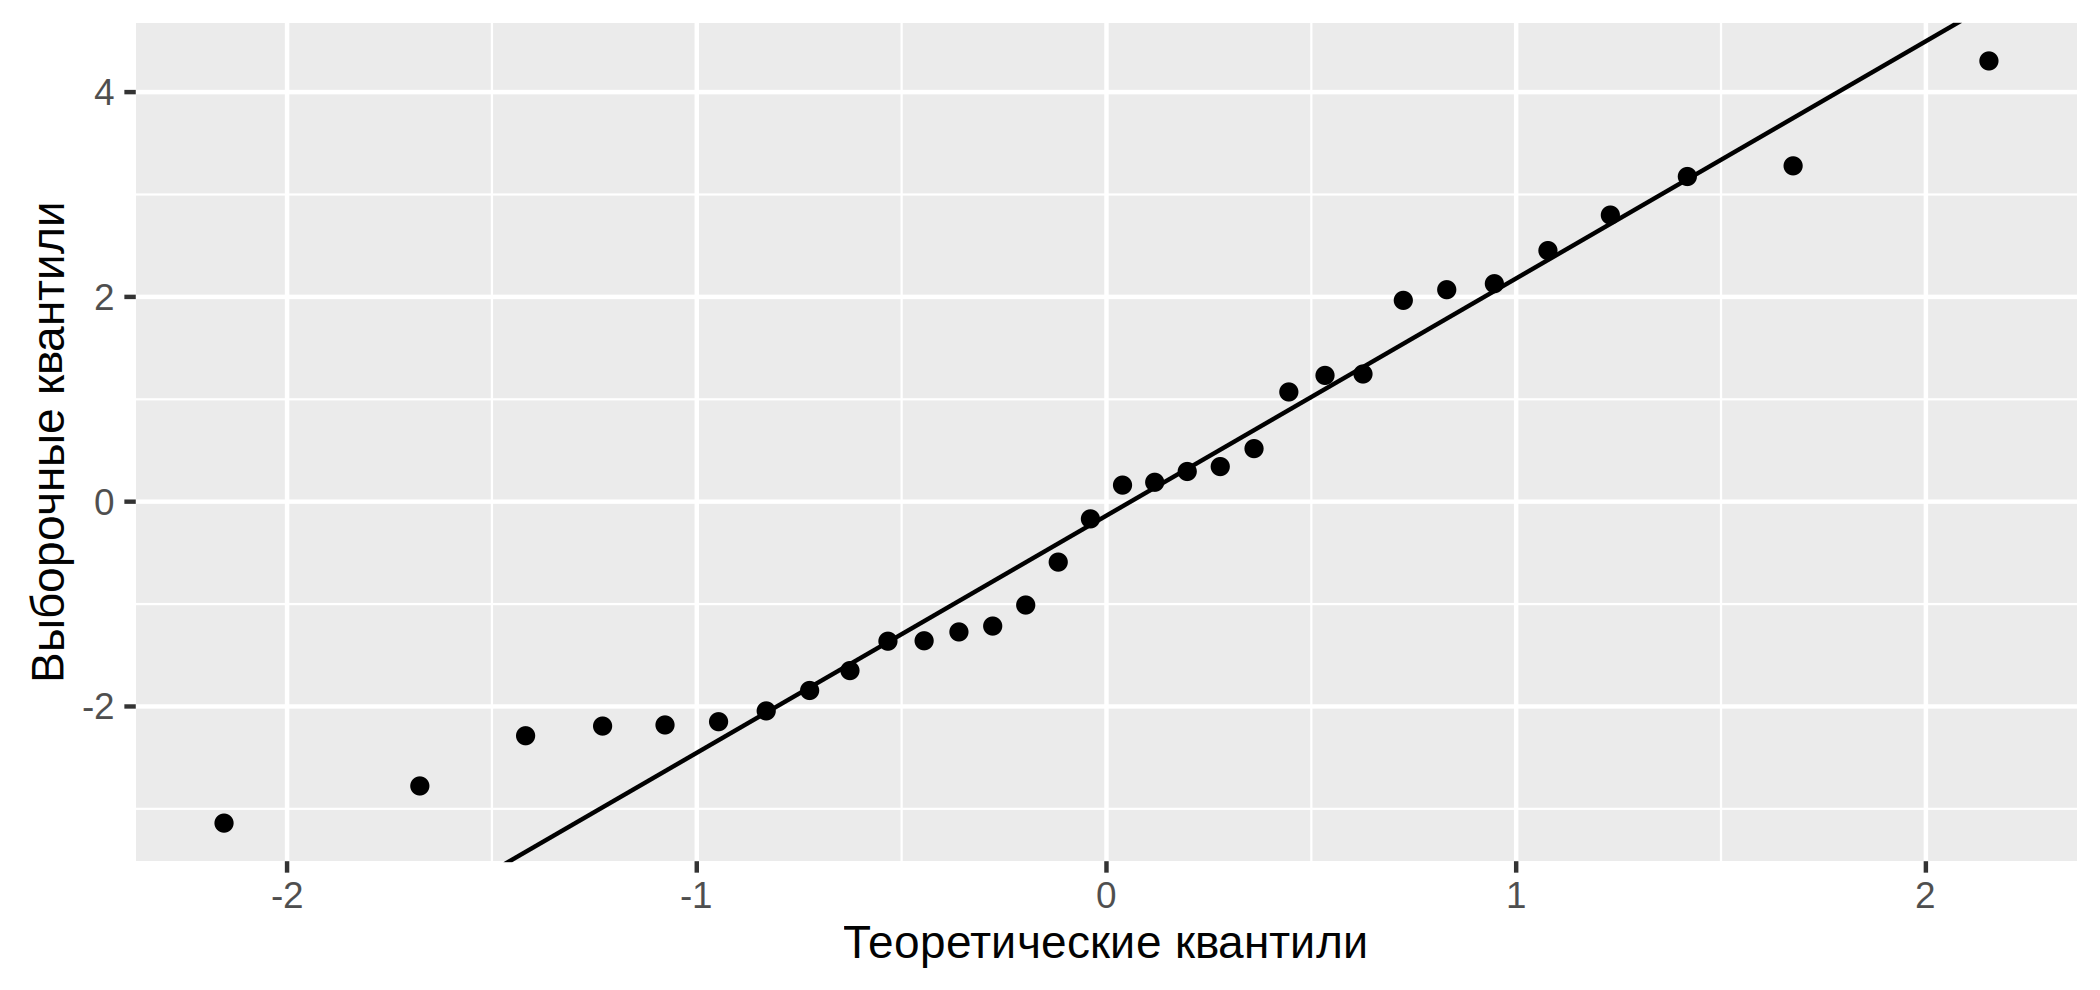
\includegraphics[width=1\linewidth]{../figures/residual/quantile.png}}
\caption{График квантилей для остатков}
\label{img:resid_qqnorm}
\end{figure}
На рисунке \ref{img:resid_qqnorm} можно заметить, что присутствуют скачки относительно нормального распределения. Наиболее явный из них --- нижний хвост. Остальные --- небольшие скачки по ходу линии нормального распределения. Проверим с помощью критерия Шапиро-Уилка, можно ли считать полученные остатки нормально распределёнными.
\begin{verbatim} 

	Shapiro-Wilk normality test

data:  data
W = 0.9513, p-value = 0.124

\end{verbatim}
В полученных результатах $W$ --- статистика Шапиро-Уилка. Вероятность ошибки $p = 0.124 > 0.05$, а значит нулевая гипотеза не отвергается. Следовательно опровергнуть предположение о нормальности на основе данного теста нельзя.

\bigskip
\bigskip
Проверим критерий $\chi^2$ Пирсона:
\bigskip
\begin{verbatim} 

	Pearson chi-square normality test

data:  data
P = 10.5143, p-value = 0.1046

\end{verbatim}
В полученных результатах $P$ --- статистика $\chi^2$ Пирсона. Вероятность ошибки $p = 0.1046 > 0.05$, а значит нулевая гипотеза не отвергается. Но при этом, это значение очень близко к $0.05$. Проверим критерий: примем уровень значимости $\alpha = 0.05$, тогда из таблицы распределения $\chi^2$ найдём критическое значение критерия $\chi_{\textrm{кр}}^2(\alpha, k) \approx 43.8$. Отсюда следует, что
\begin{equation*}
	\chi_{\textrm{набл}}^2 < \chi_{\textrm{кр}}^2,
\end{equation*}
где $\chi_{\textrm{набл}}^2 = P = 10.5143$. А значит, гипотезу о нормальности не отклоняем.

Построим график автокорреляционной функции для определения наличия взаимосвязей в ряде остатков (рисунок \ref{img:resid_acf}). На графике пунктирные линии разграничивают значимые и не значимые корреляции: значения, выходящие за линии, являются значимыми \cite[с.376]{Teetor2011RCook}.
\begin{figure}[ht]
	\center{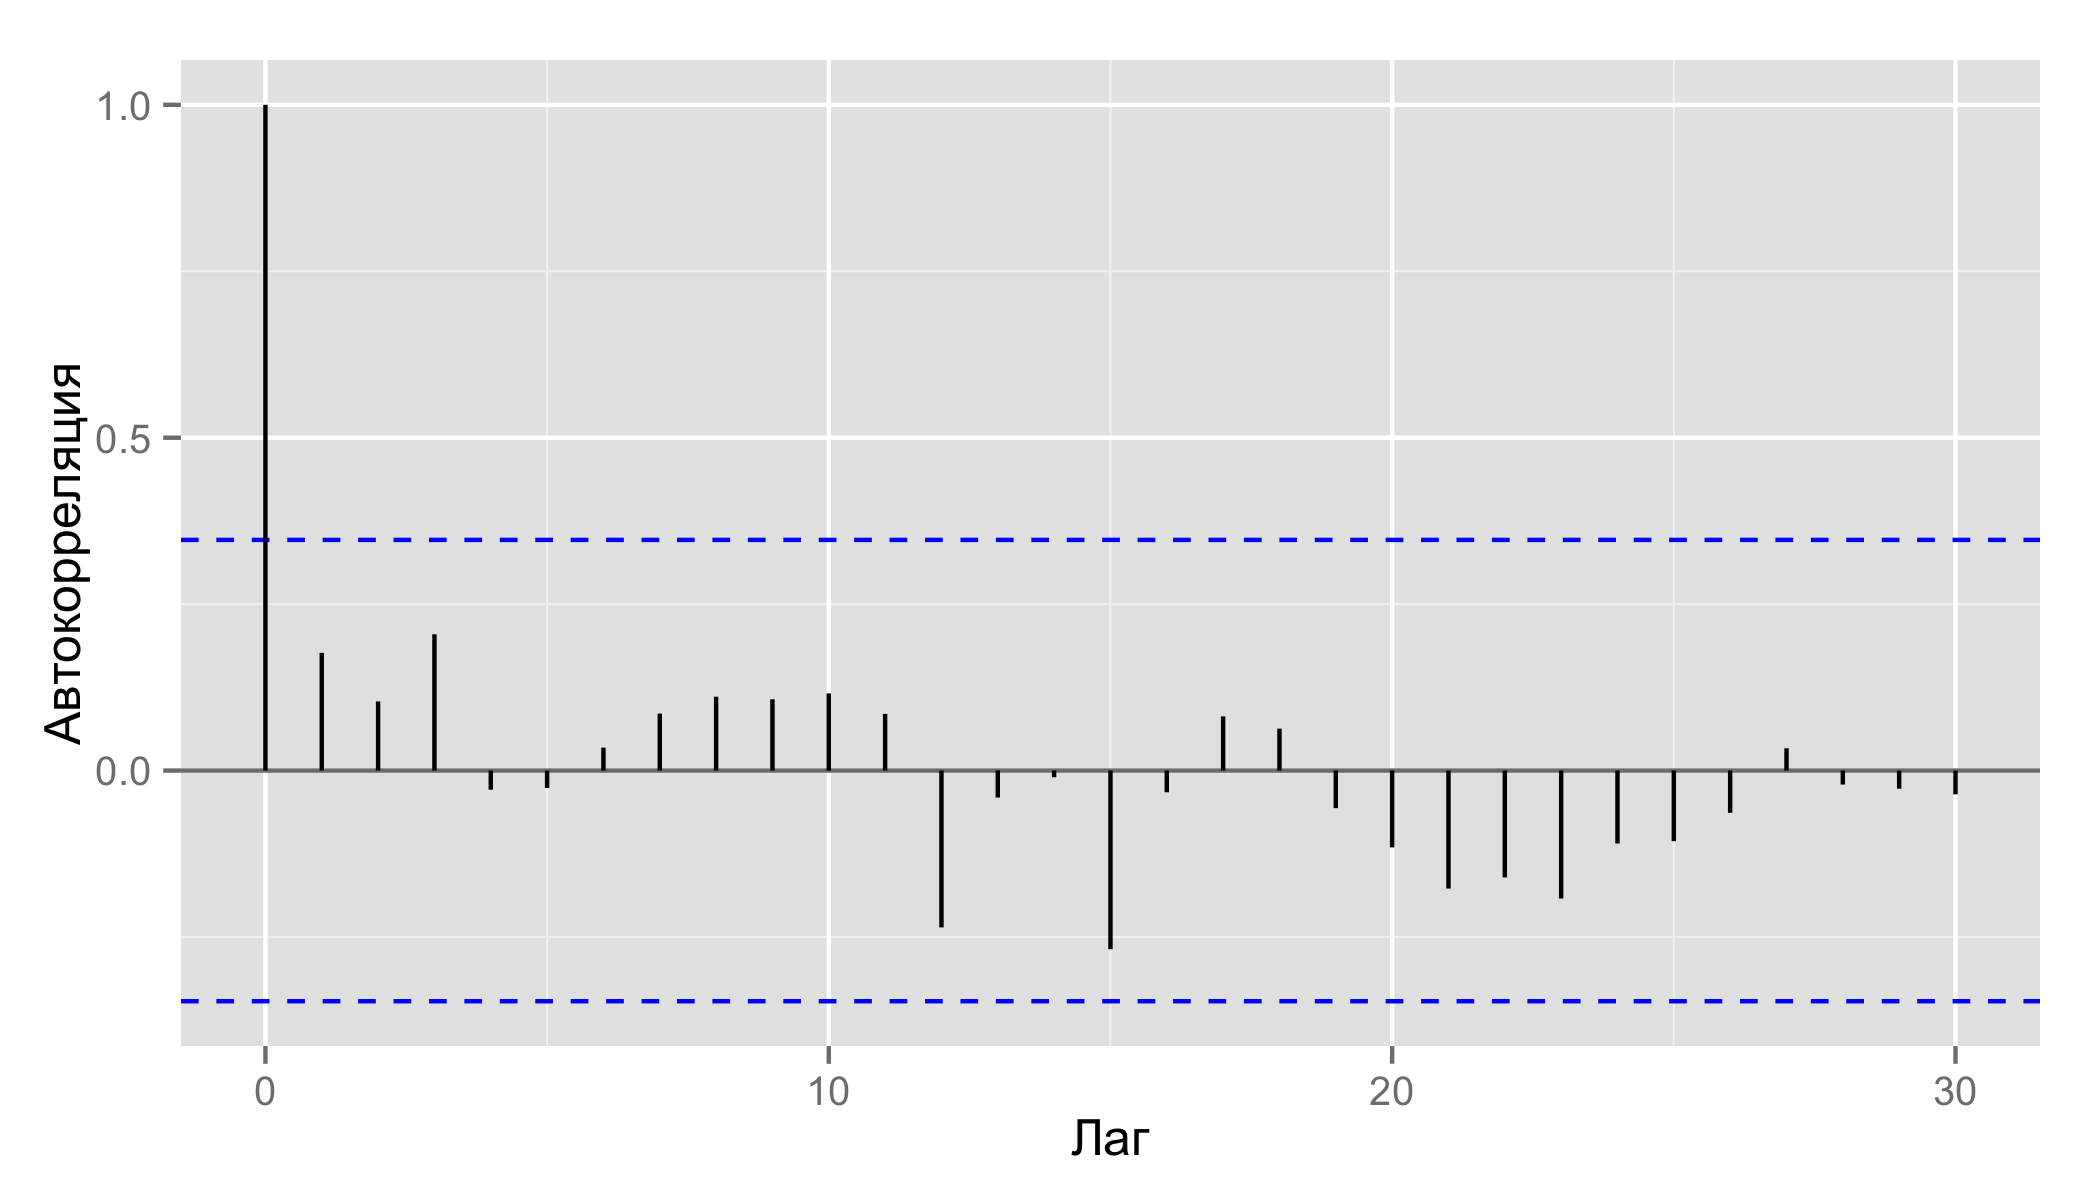
\includegraphics[width=1\linewidth]{../figures/residual/acf.png}}
\caption{График автокорреляционной функции}
\label{img:resid_acf}
\end{figure}
На представленном графике автокорреляционной функции можно заметить на лаге $15$ значение, выходящее за интервал, обозначенный пунктирными линиями. Проверим значимость автокорреляций с помощью теста Льюнга-Бокса \cite[с.377-378]{Teetor2011RCook}. Данный тест проверяет наличие автокорреляций в исследуемом ряде.
\begin{verbatim} 

	Box-Ljung test

data:  research.residuals$temperature
X-squared = 0.0754, df = 1, p-value = 0.7836

\end{verbatim}
В результатах теста $p > 0.05$, что говорит о том, что тест не выявил значимых автокорреляций.

На рисунке \ref{img:resid_acf} также можно заметить затухание с увеличением лага. На основе этого можно сделать предположение о стационарности. Для проверки этого предположения воспользуемся расширенным тестом Дики--Фуллера(ADF) \cite{Dickey1979Distribution}.
\begin{verbatim} 

	Augmented Dickey-Fuller Test

data:  research.residuals$temperature
Dickey-Fuller = -3.2695, Lag order = 3, p-value = 0.09261
alternative hypothesis: stationary

\end{verbatim}
Как видно из результатов проверки теста, $p < 0.05$. Следовательно, необходимо принять альтернативную гипотезу о стационарности.

Полученная модель получилась неоднозначной, с одной стороны, полученное значение коэффициента детерминации показало недостаточную точность полученной модели и не удалось достоверно показать нормальность ряда остатков. С другой стороны, была показана стационарность и отсутствие автокорреляции. Поэтому возникает необходимость строить модель другими методами.

% section regr_analysis (end)

\section{Вариограммный анализ. Кригинг.} % (fold)
\label{sec:_variogram}

В данной части работы для более объективного оценивания полученных прогнозов возьмем в качестве исследуемой выборки первые $32$ значения исходных данных.

Традиционные детерминированные методы, широко используемые в задачах прогнозирования, в большинстве случаев на практике не позволяют в полной мере решить ту или иную задачу. В наиболее благоприятных вариантах исследований они позволяют оценивать значения в точках, в которых измерения не проводились и определять значения на плотной сетке (в близких к измерениям точках). Следует также отметить, что данные измерений, как правило, дискретны и неоднородно распределены. В свою очередь, анализ этих данных и его результаты в значительной мере зависят как от качества так и от количества исходных данных. И именно такие выводы были сделаны в результате проделанной в предыдущих частях данной работы. Отсюда следует, что необходимо использовать другие современные методы, позволяющие сделать более точные модели и выводы.

Для поставленной задачи в современных исследованиях хороших результатов позволяет добиться методы геостатистики, что подтверждается работами \cite{GeoStCompar1987, GeoStCompar1998}. Современная геостатистика --- это широкий спектр статистических моделей и инструментов для анализа, обработки и представления пространственно-распределенной информации.

В рамках геостатистики, для получения наилучшей в статистическом смысле пространственной оценки используются модели из семейства кригинга (\textit{kriging}) --- наилучшего линейного несмещенного оценивателя (\textit{Best Linear Unbiased Estimator --- BLUE}). Кригинг является ``наилучшим'' оценивателем в статистическом смысле --- его оценка обладает минимальной дисперсией. Важным свойством кригинга является точное воспроизведение значений измерений в имеющихся точках (интерполяционные свойства). В отличие от многочисленных детерминированных методов оценка кригинга сопровождается оценкой ошибки интеполяции в каждой точке. Полученная ошибка позволяет охарактеризовать неопределенность интерполяционноий оценки данных при помощи доверительных интервалов.

В отличие от детерминированных методов, геостатистические оценки опираются на информацию о внутренней структуре данных, зависят от самих данных, т. е. являются адаптивными.

Центральная идея геостатистики состоит в использовании знаний о пространственной корреляции экспериментальных данных для построения пространственных оценок и интерполяций. Вариограмма --- ключевой инструмент для оценки степени пространственной корреляции, имеющейся в данных, и для ее моделирования. Модель вариограммы является функцией, определяющей зависимость изменения исследуемой величины в пространстве от расстояния. Следовательно, интерполяционная модель, основанная на такой корреляционной функции, будет отражать реальные явления, которые лежат в основе данных измерений. Всевозможные пары точек могут быть рассортированы по классам в соответствии с разностью их координат $ h = x_i - x_j $, называемой \textit{лагом}. Для близких точек разность значениеq функции в них обычно меньше и растет с увеличением расстояния между точками. Вычислив среднее значение квадратов разностей для каждого значения лага $h$ (для каждого собранного класса пар измерений), можно получить дискретную функцию, называемую \textit{экспериментальной вариограммой}. Вариограмма обычно характеризуется тремя значениями: эффект самородков(\textit{nugget}), ранг(\textit{range}) и порог(sill). Эффект самородков характеризуется разрывом вариограммы около нуля. Порог характеризует предельное значение вариограммы, на некотором расстоянии, называемом рангом, за которым последующие значения вариограммы становятся некоррелированными.

Также при построении вариограммы следует учитывать параметр максимального расстояния, для которого вычисляется вариограмма. Первоначальным параметром было выбрано следующее значение: $ 2n / 3 = 21 $ \cite{cressie2011statistics}.

Построим экспериментальную вариограмму с помощью пакета \textit{gstat} и функции \textit{variogram}. С помощью этой функции можно построить экспериментальную вариограмму, основанную на классической оценки вариограммы и робастной оценки Кресси \cite{cressie2011statistics}. Построим экспериментальную вариограмму с помощью классической оценки.

\begin{figure}[ht]
	\center{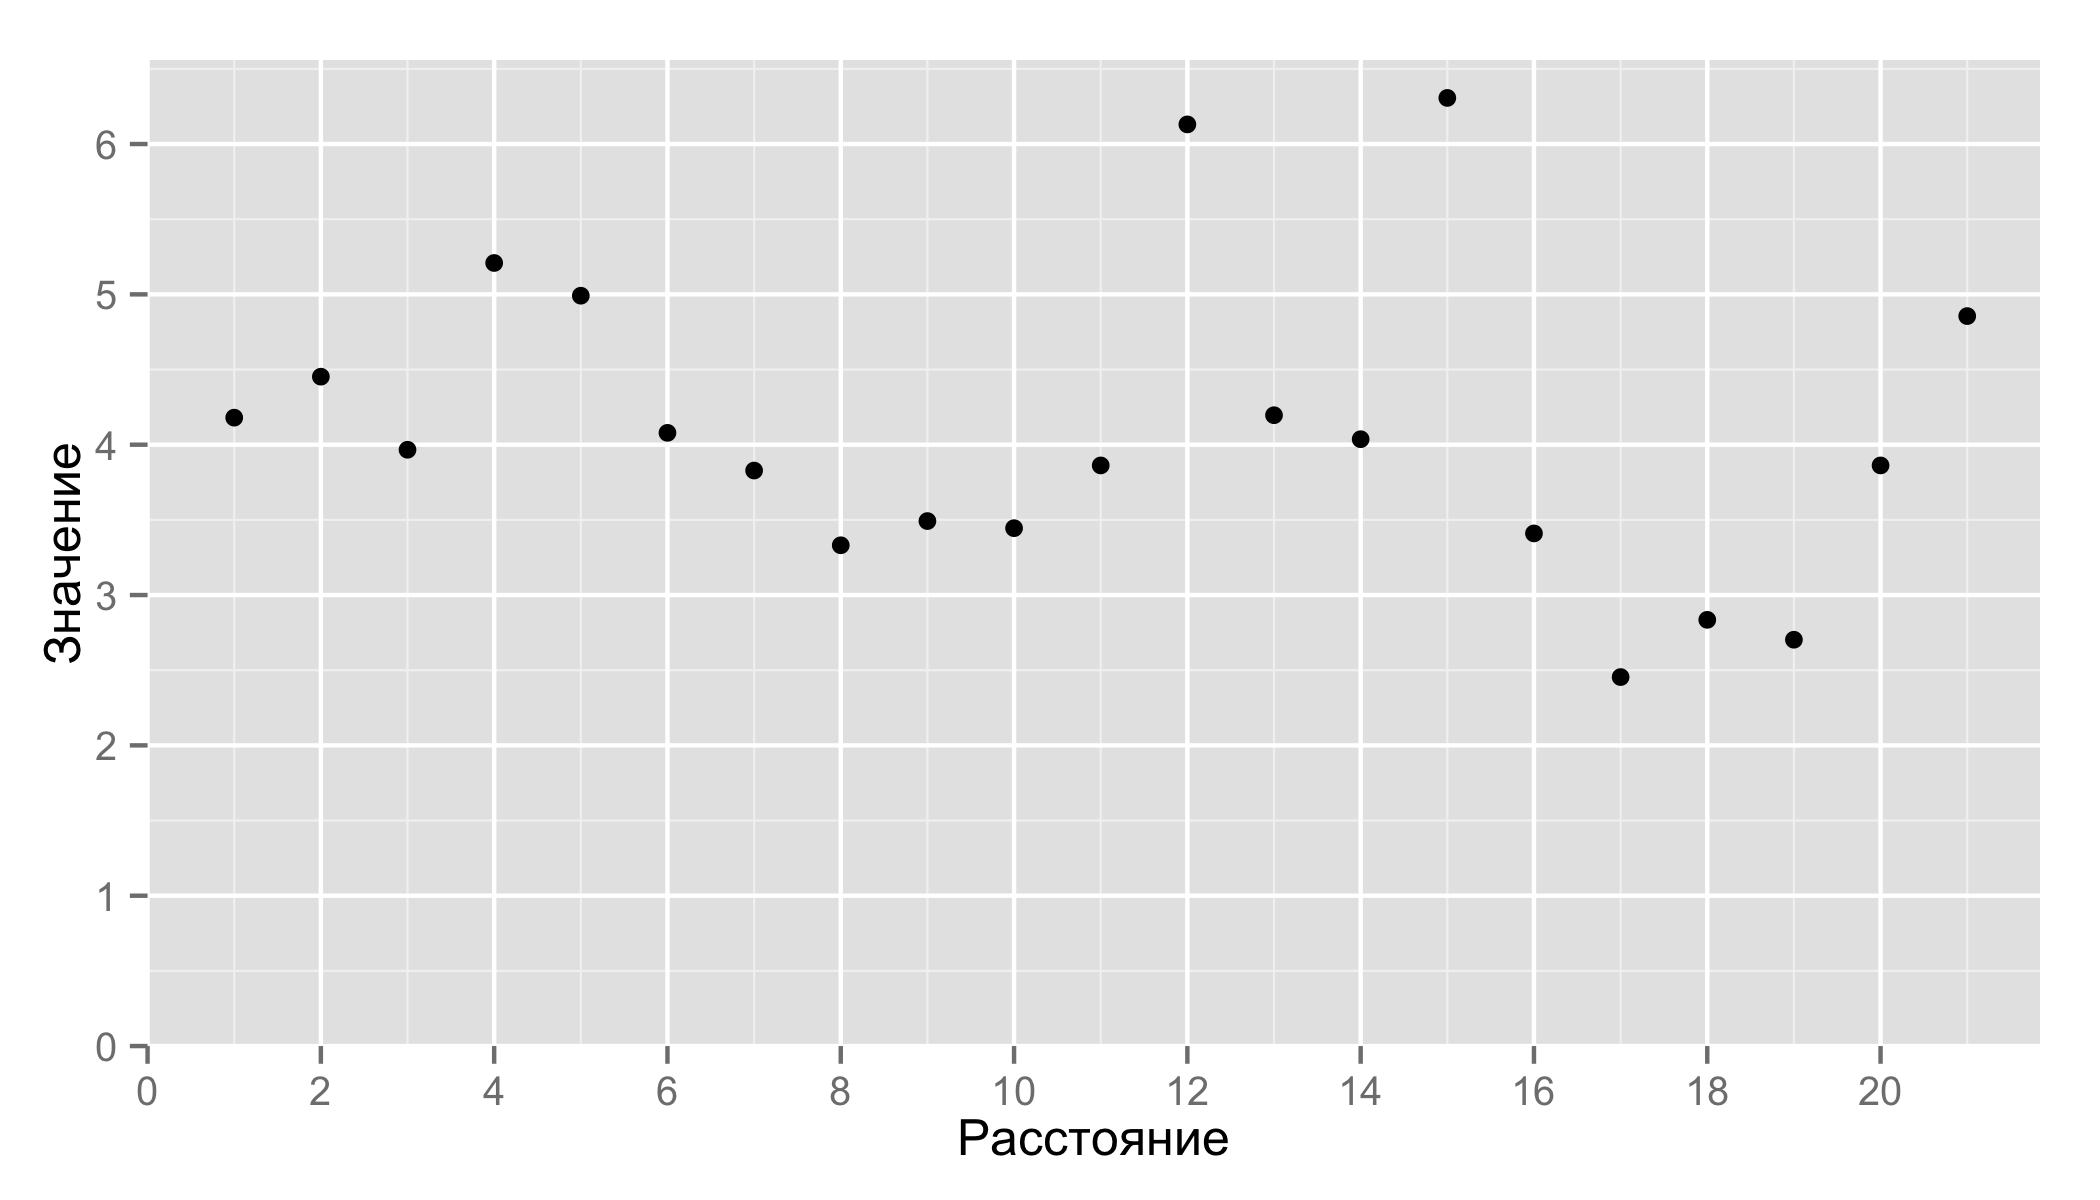
\includegraphics[width=1\linewidth]{../figures/variogram/classical-empirical.png}}
\caption{Экспериментальная вариограмма}
\label{img:classical_emp}
\end{figure}

Построенная вариограмма отображена на рисунке \ref{img:classical_emp}. На представленном рисунке можно заметить, что на промежутке $[0;1]$ не происходит роста значений вариограммы. Наоборот, наблюдается разрыв: первое значение находится значительно выше $0$. При этом вариограмма не сильно выходит за пределы дисперсии переменной, которая равна $4.07$. Более того, первые значения уже достигло порога. Что говорит о том, что вариограмма на первых значениях выходит на предельное значение, и последующие значения некоррелированы. Это, на самом деле, согласуется с нашими исходными данными, так как при анализе остатков было выявлено отстутсвие автокорреляций, и спецификой самих данных: наблюдение за каждый год, вообще говоря, не зависит от предшедствующего.

На основе этого делаем вывод о наличии эффекта самородков и делаем первоначальное предположение о равенстве порога $3.9$.

На основе экспериментальной вариограммы построим модель вариограммы для дальнейшего использования на этапе кригинга. Моделью вариограммы может служить не каждая функция, а только та, для которой выполнено условие положительной определенности. Положительная определенность модели вариограммы гарантирует, что уравнения кригинга, построенные с использованием данной модели, имеют единственное устойчивое решение. Поэтому при моделировании используются только те функции, для которых положительная определенность установлена, а также их взвешенные линейные комбинации с неотрицательными весами, которые тоже будут являться положительно определенными. Модель вариограммы строится как линейная комбинация подходящих базисных моделей \cite{saveliev2012}.

Для построения моделей вариограммы существует два подхода: вручную, т.е. визуально с ручным подбором параметров, и автоматическим подбором параметров с помощью специальных методов. И на практике построение модели вариограммы представляет собой итеративный процесс, на каждом шаге которого следует наилучшим образом подобрать параметры очередного модельного приближения. В различной литературе рекомендуется строить моделей вручную, так как исследователь лучше знает специфику данных, чем различные методы оценивания. Попробуем построить модель вариограммы визуально.

Ранее было отмечено присутствие эффекта самородков. Другой, часто встречающейся моделью, является сферическая:
\begin{equation}
	\gamma(\vert h \vert) = c Sph_a(\vert h \vert) = \left\{
 \begin{array}{l l}
   c(1.5 \vert h \vert / a - 0.5(\vert h \vert / a)^3) &, \vert h \vert \le a, \\
   \\
   c &,	 \vert h \vert > a.
 \end{array} \right.
\end{equation}

Возьмём эту модель в качестве базовой с помощью функции \textit{vgm}, в качестве начального параметра возьмём порог, указанный ранее: $3.9$. Далее воспользуемся функцией \textit{fit.variogram} для подбора более точных значений указанной модели. Таким образом окончательная модель:
% latex table generated in R 3.1.3 by xtable 1.7-4 package
% Sat May 30 20:33:43 2015
\begin{table}[H]
\centering
\begin{tabular}{rlrr}
  \hline
 & Модель & Порог & Ранг \\ 
  \hline
1 & Nug & 0.00 & 0.00 \\ 
  2 & Per & 4.10 & 0.90 \\ 
   \hline
\end{tabular}
\caption{Модель вариограммы} 
\label{table:manual_model}
\end{table}

И график полученной модели на рисунке \ref{img:var-models} (пунктиром). На графике можно проследить все указанные ранее особенности: эффект самородков и порог.
\begin{figure}[ht]
	\center{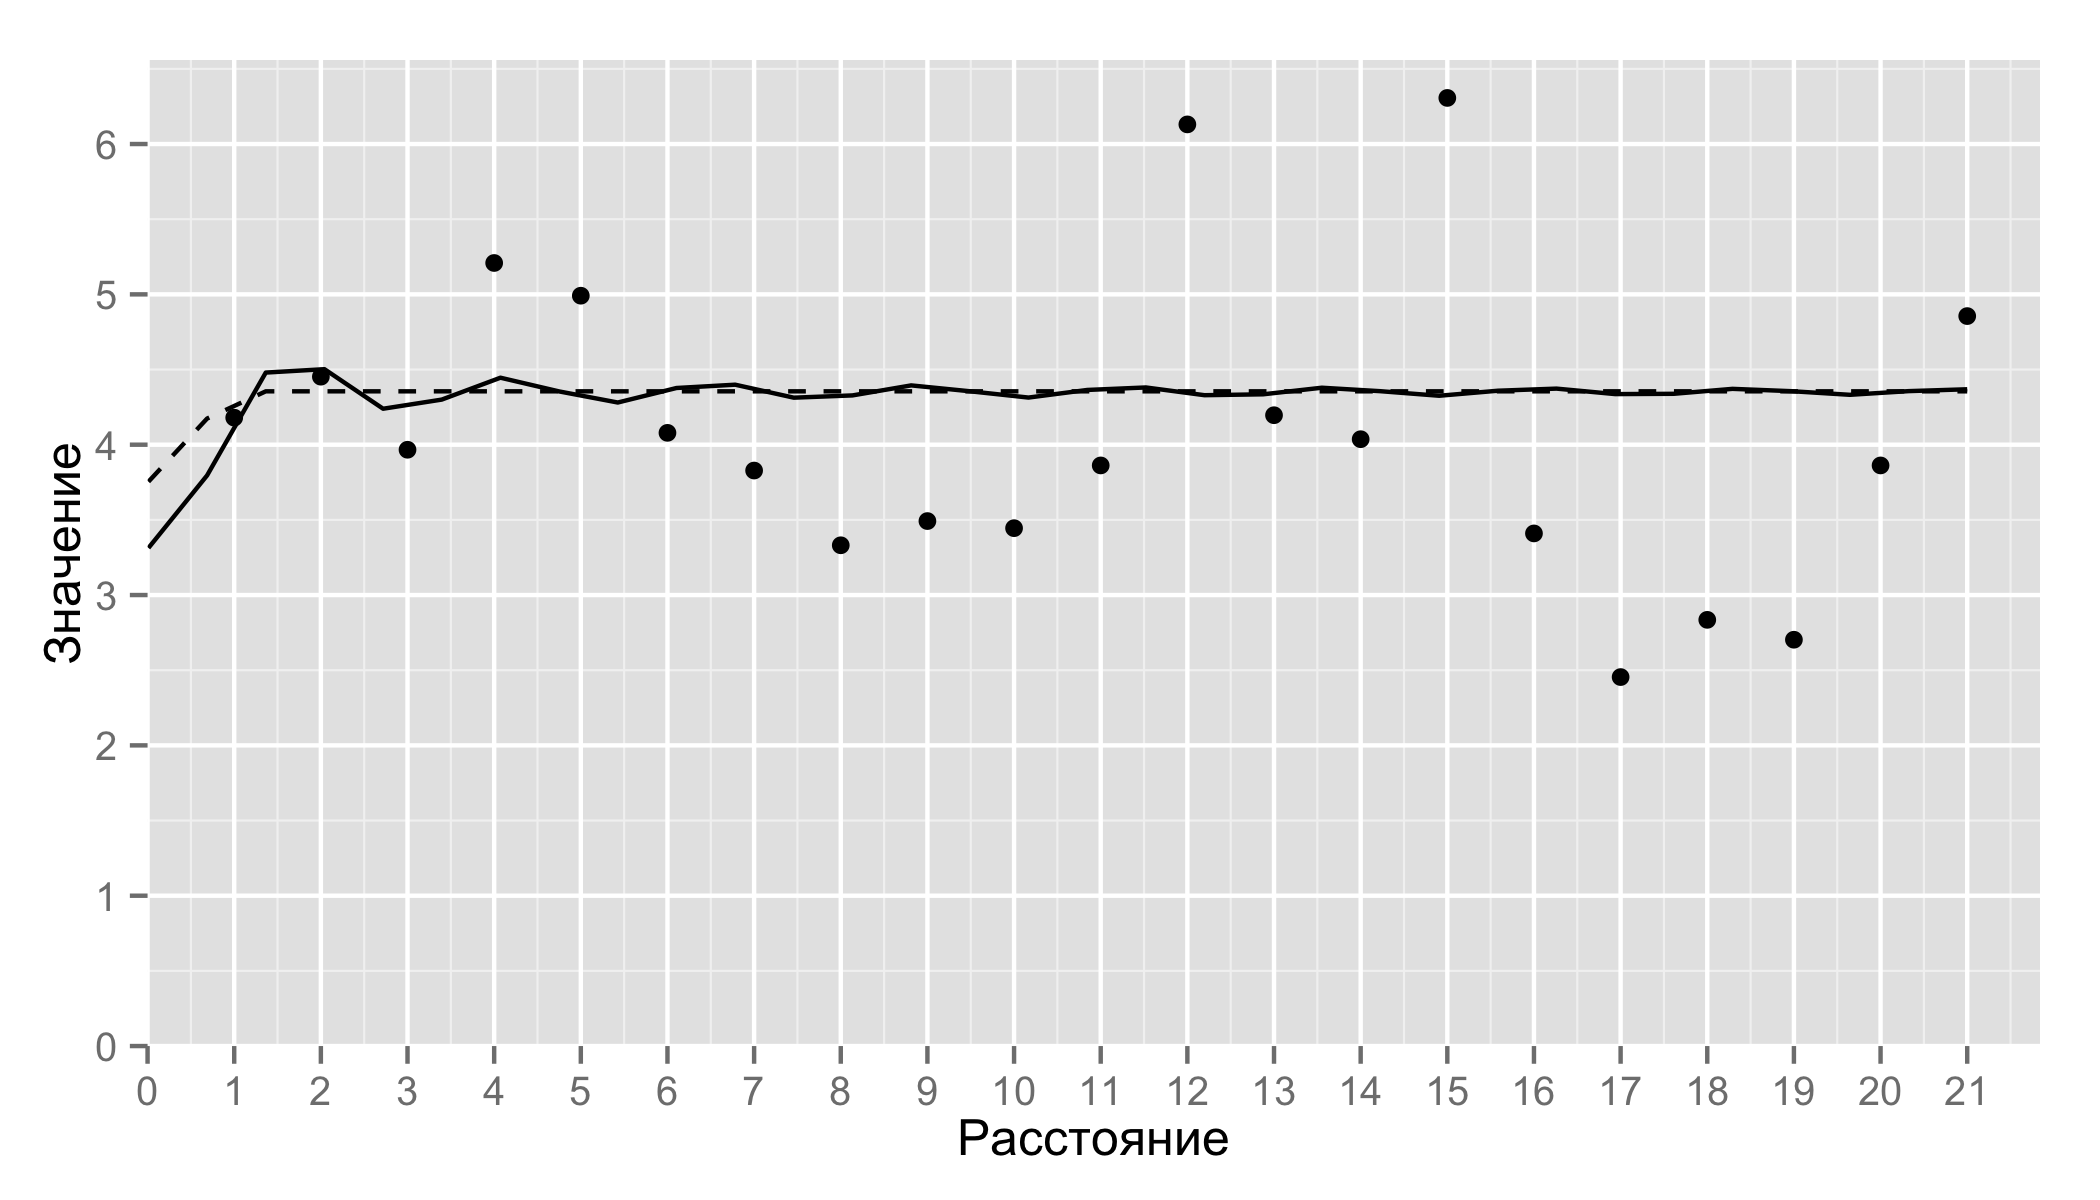
\includegraphics[width=1\linewidth]{../figures/variogram/models-comparison.png}}
\caption{Модели классической вариограммы}
\label{img:var-models}
\end{figure}

Задача геостатистики --- оценить значения изучаемой пространственной переменной в произвольных точках области исследования на основе анализа ее значений, измеренных в ограниченном числе выборочных точек. По построенной модели вычислим оценки при помощи ординарного кригинга, реализованного функцией \textit{krige}. Вычисленные значения: $-0.0011039642,  0.0007688937,  0.0007688937,  0.0007688937,  0.0007688937,  0.0007688937$. Оценку отклонения от истинных значений выразим с помощью среднеквадратической ошибки \textit{(MSE)}. В данном случае $ MSE = 2.622 $. Полученные значения оказались очень близкими к нулю и, начиная со второго значения значения не изменяются. Следовательно прогноз почти не изменился. Это говорит о том, что построенная модель не смогла уловить поведение исходных данных. По этой причине был использован второй вариант построения модели --- c автоматическим подбором параметров.

Для построения модели вариограммы была реализована возможность автоматического подбора модели на основе функции \textit{fit.variogram}. Суть этого подхода заключается в следующем: при заданных начальных условиях (эффект самородков, ранг, порог), для всех возможных базисных моделей подгонялись их параметры, для этих моделей вычислялись сумма квадратов ошибок, и на основе этого показателя выбиралась наиболее эффективная модель. Код программы представлен в листинге \ref{lst:main}.

На рисунке \ref{img:var-models} сплошной линией показан результат выполнения представленной ранее функции. Таким образом, наилучшей моделью вариограммы, построенной по классической оценке, стала линейная комбинация двух: эффект самородков с параметром $3.3129$ и модель с эффектом дыр (\textit{Hole}) с параметрами: порог --- $1.039$, ранг --- $0.379$.

Методом кригинга в этом случае были построены следующие прогнозные значения: $0.136405083, -0.109638356,  0.083961891 -0.030572187, -0.002709375,  0.045735285$. Полученные значения отличаются от предыдущих, в них появилось некоторое поведение. Но в данном случае $ MSE = 2.82 $, что хуже предыдущего значения, а значит, прогноз ухудшился.
Попробуем улучшить результат с помощью робастной оценки Кресси.

\begin{figure}[ht]
	\center{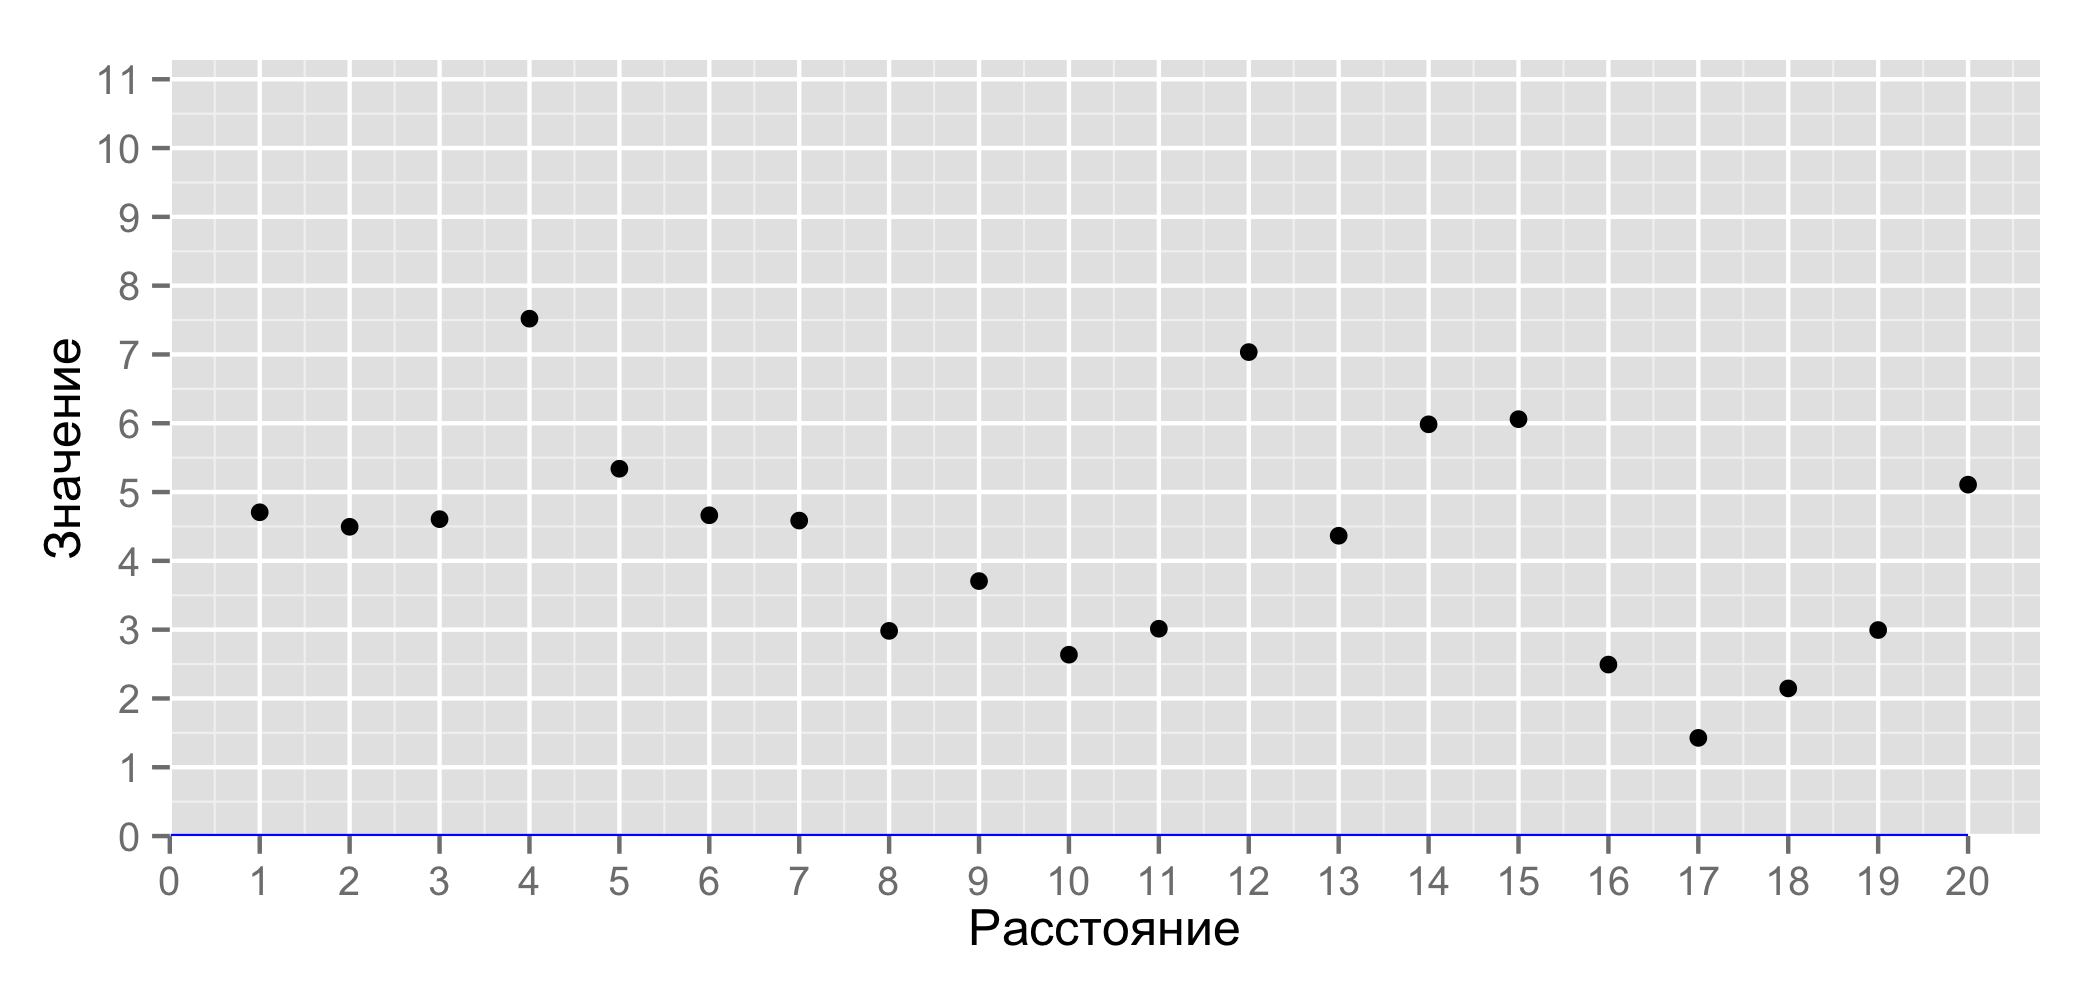
\includegraphics[width=1\linewidth]{../figures/variogram/robust-modeled.png}}
\caption{Теоретическая вариограмма (робастная оценка)}
\label{img:robust-mod}
\end{figure}

Модель вариограммы, представленная на рисунке \ref{img:robust-mod}, является также линейной комбинацией двух базисных моделей: эффекта самородков с параметром $ 4.002625 $ и волновая модель с параметрами: $0.316283$, $2.985461$. Заметим, что эмпирическая вариограмма, построенная по робастной оценке, отличается от соотвествующей вариограмм, построенных по классической оценке. Появилось заметное поведение вариограммы, в отличие от предыдущей, где значения концентрировались около дисперсии выборки.

Результаты кригинга показали следующие прогнозные значениея: $0.02145686, 0.11662121, 0.08211072, -0.01052573, -0.06521018, -0.04189881$. Среднеквадратическая ошибка $ MSE = 2.654 $, таким образом это значение близко к значению, полученному вручную. Таким образом, использование робастной оценки улучшило результат применения кригинга.

\begin{figure}[H]
	\center{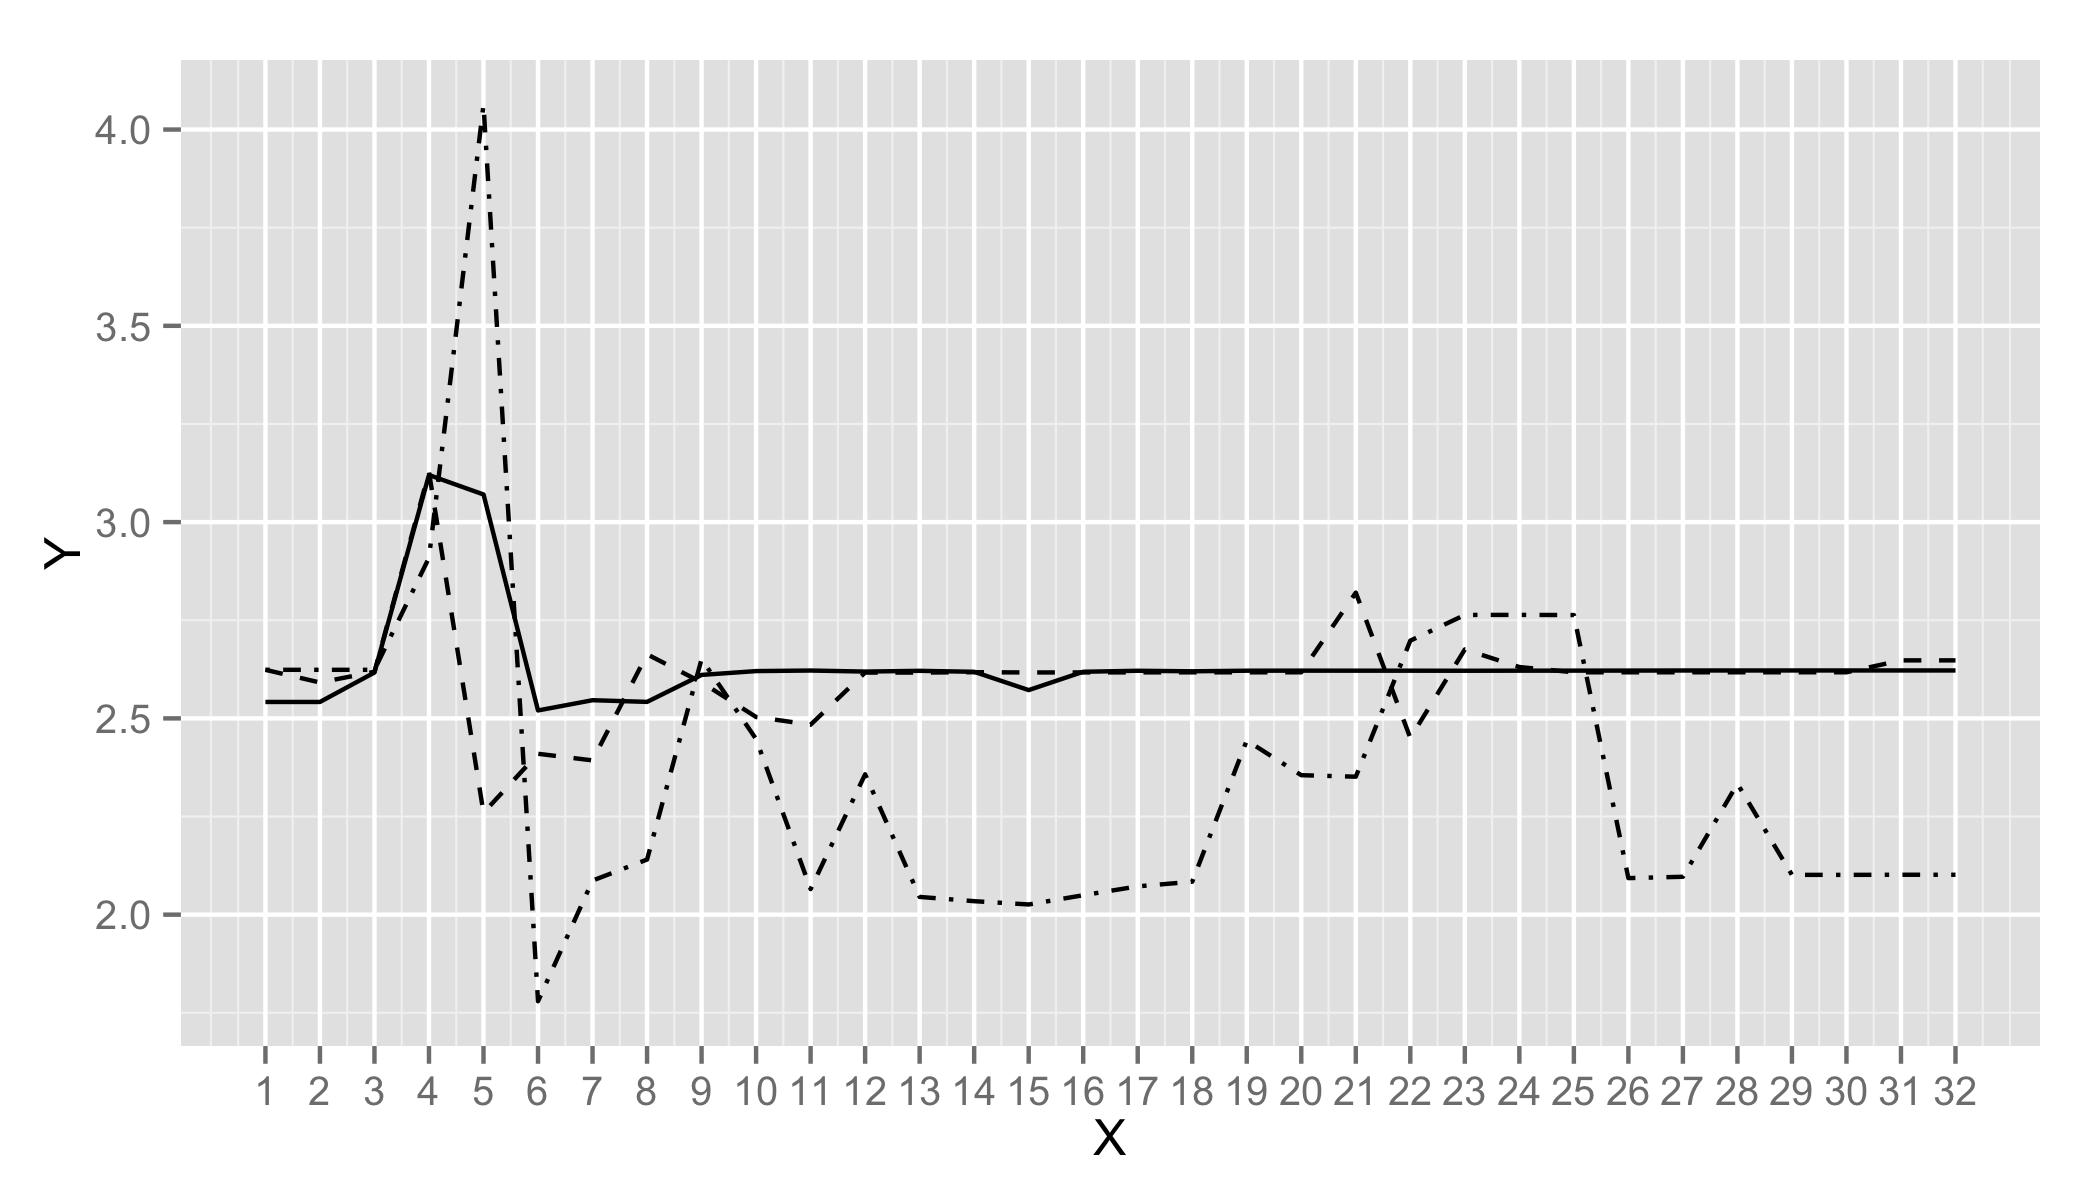
\includegraphics[width=1\linewidth]{../figures/variogram/parameter-comparison.png}}
\caption{Зависимость ошибки от максимального расстояния}
\label{img:check-dep}
\end{figure}

Исследуем теперь поведение кригинга при различных параметрах максимального расстояния вариограммы. В качестве оценки качества полученного прогноза возьмем среднеквадратическую ошибку. Чем меньше ошибка --- тем лучше прогноз. Для этих целей реализована функция \textit{checkDepByMSE}. Результат её работы на рисунке \ref{img:check-dep}. На этом графике четко видно, что робастная оценка (пунктир-точка), в отличие от классической (пунктир) и модели, построенной вручную (сплошная), в большинстве случаев даёт более точные прогнозы. И наилучший при максимальном расстоянии равным $6$. С этим параметром, наилучший прогноз составляют значения кригинга: $-0.42389948, -0.06109632, 0.24895664, 0.39591184, 0.34950710, 0.16404797$. Среднеквадратическая ошибка составляет $1.779479$.

\begin{figure}[H]
\center{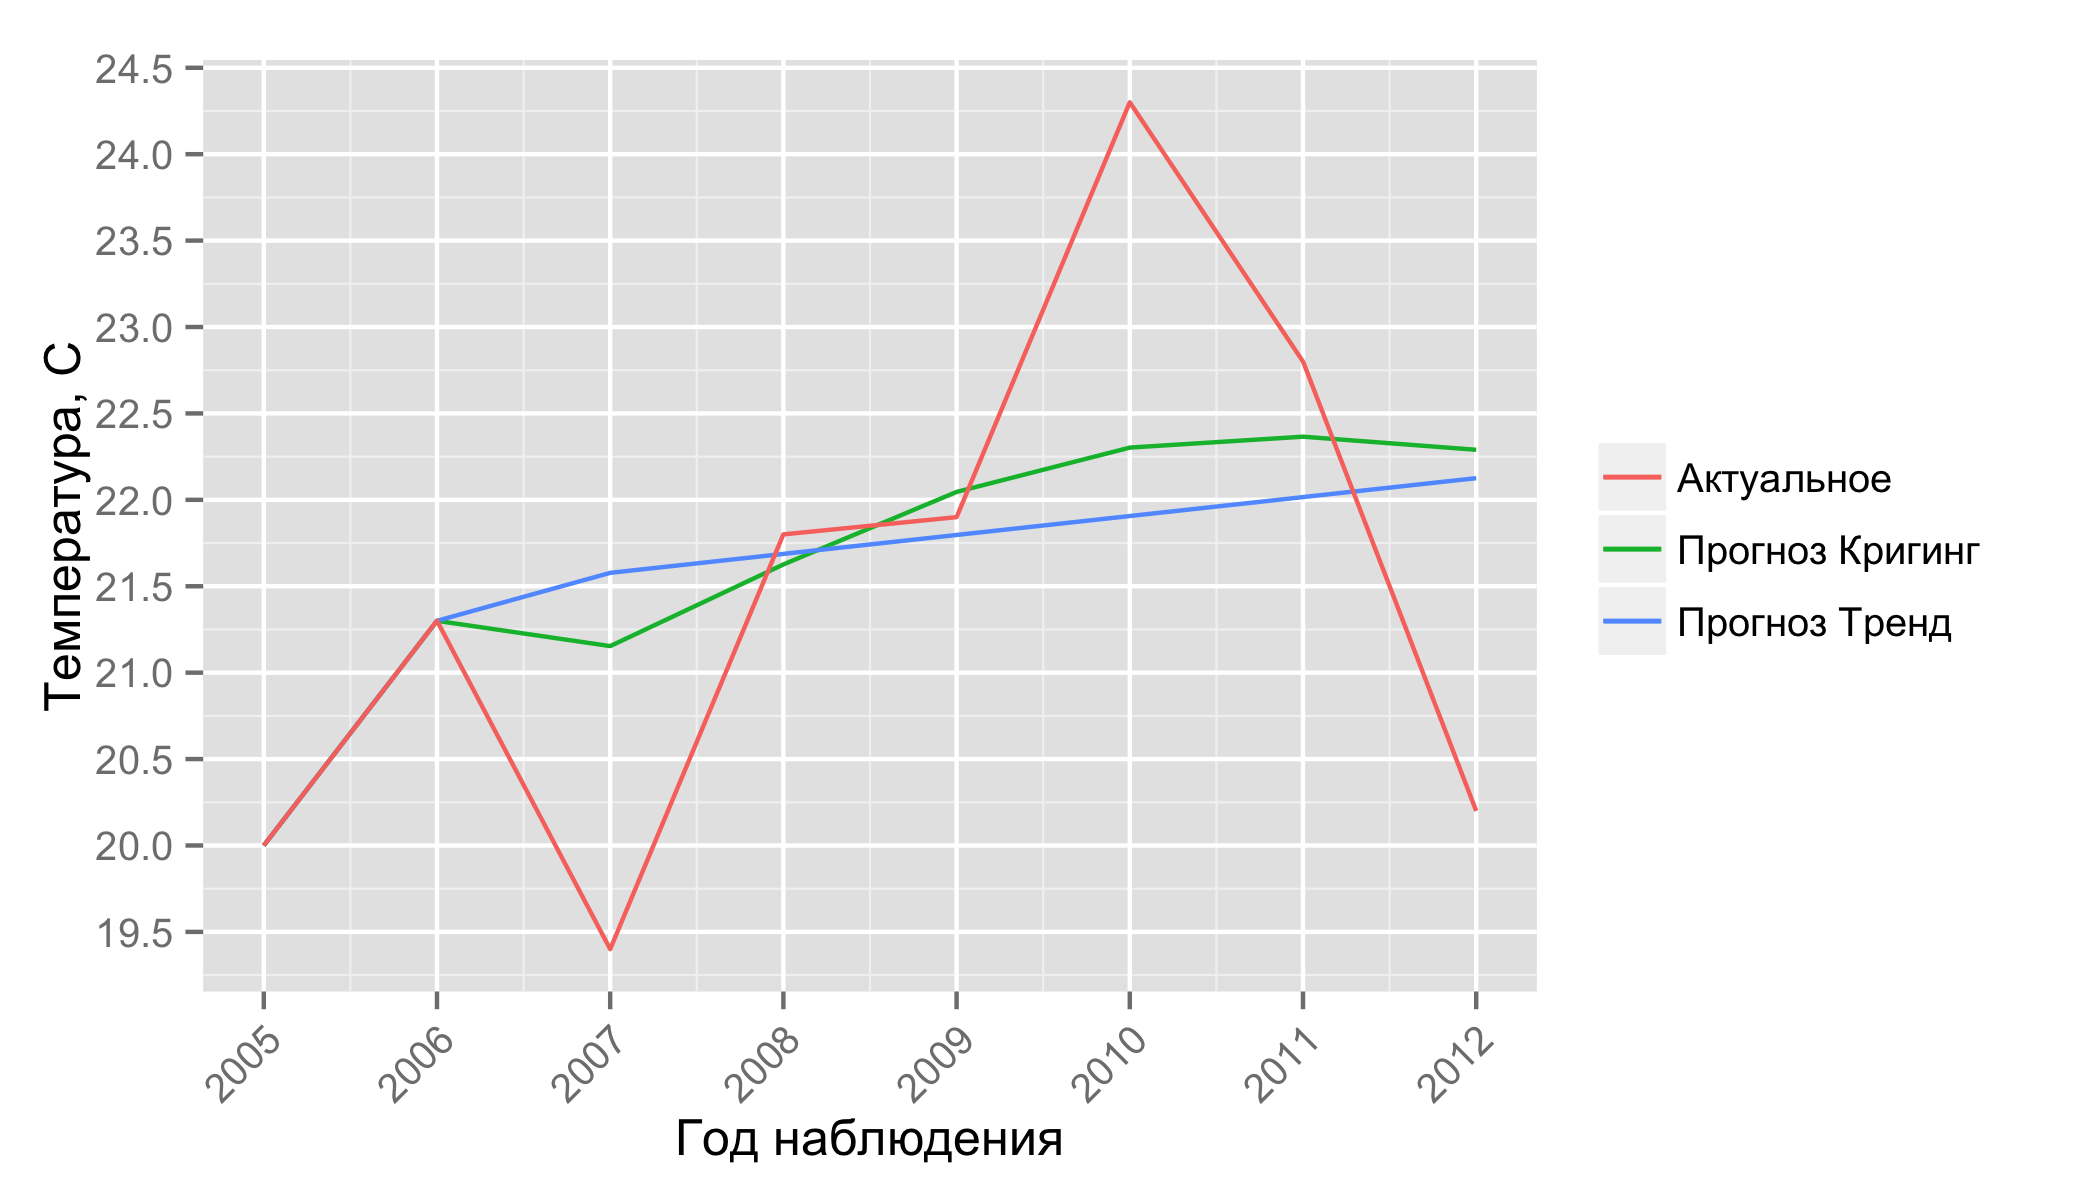
\includegraphics[width=1\linewidth]{../figures/variogram/cross-prediction-robust-best.png}}
\caption{Сравнение прогнозных значений}
\label{img:cross-prediction-best}
\end{figure}

Сравнительный анализ полученного прогноза на графике \ref{img:cross-prediction-best}.

Таким образом в результате вариограммного анализа были исследованы различные модели вариограмм, оценки, проведены два подхода по вычислению. В результате кригинга построена наилучшая модель прогнозных значений. Которая в свою очередь имеет погрешность в пределах стандартного отклонения. Следовательно данная модель является хорошим вариантом для построения прогнозных значений.
% section _variogram (end)

  %\chapter*{Заключение}
\addcontentsline{toc}{chapter}{Заключение}

В представленной работе бы проведён сравнительный анализ современных пакетов прикладных программ для статистического анализа. Из них как инструмент исследования был выбран язык программирования \textbf{R}, по причине его доступности и предоставления огромного числа пакетов. С помощью этого пакета была исследована важнейшая характеристика любого водоёма --- температура воды. Исследование проводилось на основе данных, полученных из наблюдений за озером Баторино, в период с 1975 по 2012 год в июле месяце. Для этого были вычислены и проанализированы описательные статистики, проведена проверка на нормальность, проведён визуальный анализ. В результате указанной части работы было обнаружено, что распределение температуры воды в озере Баторино близко к номральному закону распределения с параметрами $\mathcal{N}(20.08, 5.24)$. Отклонение от нормальности отмечается полученными коэффициентами асимметрии и эксцесса. Исследуемое распределение имеет небольшую скошенность вправо и более растянутую колоколообразную форму относительно нормального закона распределения. В результате проведённого корреляционного анализа была выявлена умеренная зависимость между температурой воды и временем: был обнаружен рост температуры с течением времени.

В работе, как заключительный этап исследования, был проведён регрессионный анализ. В процесса которого была построена аддитивная модель временого ряда, найдён тренд, и, как следствие удаления тренда из построенной модели, был получен ряд остатков. Построенная детерминированными методами линейная регрессионная модель оказалась значимой и адекватной, но при этом описывает поведение временного ряда лишь частично. В результате анализа ряда остатков было выявлено отклонение распределения от нормальности. Что говорит о наличии некоторых неучтённых данной моделью факторов, затрудняющих дальнейшее исследование классическими методами. Следует также отметить стационарность и отсутствие автокорреляций в ряде остатков. Эти результаты говорят о постоянстве вероятностных свойств с течением времени, а также об отсутствии зависимостей между наблюдениями.

В заключение хотелось бы отметить, что представленные в данной работе классические методы анализа временных рядов, в этом случае оказались недостаточными для полноценного исследования. Поэтому в дальнейшем исследовании следует использовать отличные от использованных в работе современные методы анализа.
  % \bibliographystyle{unsrt}
\bibliography{bibdb}
\addcontentsline{toc}{chapter}{Литература}
  % %!TEX root = thesis.tex

\newpage

\makeatletter
\renewcommand\appendixname{Приложение}
\gdef\appendix{\par
\setcounter{section}{0}%
\setcounter{subsection}{0}%
\def\thesection{\@Alph\c@section}
\def\section##1{\refstepcounter{section}
\setcounter{table}{0}
\def\thetable{\@Alph\c@section.\arabic{table}}
\goodbreak\noindent{\indent\Large\bf\hbox to 8.5em{\appendixname\
\thesection\hss}\hspace{0.8ex}##1}%
\nobreak\vspace{1em}\nobreak\noindent%

\addcontentsline{toc}{chapter}{\hbox to 8.5em{\appendixname\ \thesection\hss}\hspace{0.8ex}##1}}}
\makeatother

\appendix

\section{ Исходные данные}
\label{c:source_data}
% latex table generated in R 3.1.2 by xtable 1.7-4 package
% Tue Mar  3 10:11:27 2015
\begin{table}[H]
\centering
\begin{tabular}{rrr}
  \hline
 & year & temperature \\ 
  \hline
1 & 1975.00 & 20.20 \\ 
  2 & 1976.00 & 16.00 \\ 
  3 & 1977.00 & 17.70 \\ 
  4 & 1978.00 & 16.75 \\ 
  5 & 1979.00 & 17.50 \\ 
  6 & 1980.00 & 16.77 \\ 
  7 & 1981.00 & 19.80 \\ 
  8 & 1982.00 & 19.00 \\ 
  9 & 1983.00 & 21.40 \\ 
  10 & 1984.00 & 19.40 \\ 
  11 & 1985.00 & 20.40 \\ 
  12 & 1986.00 & 16.50 \\ 
  13 & 1987.00 & 17.10 \\ 
  14 & 1988.00 & 23.80 \\ 
  15 & 1989.00 & 19.90 \\ 
  16 & 1990.00 & 18.50 \\ 
  17 & 1991.00 & 23.00 \\ 
  18 & 1992.00 & 21.90 \\ 
  19 & 1993.00 & 18.00 \\ 
  20 & 1994.00 & 21.40 \\ 
  21 & 1995.00 & 18.90 \\ 
  22 & 1996.00 & 19.10 \\ 
  23 & 1997.00 & 21.00 \\ 
  24 & 1998.00 & 18.40 \\ 
  25 & 1999.00 & 23.50 \\ 
  26 & 2000.00 & 21.00 \\ 
  27 & 2001.00 & 24.20 \\ 
  28 & 2002.00 & 23.10 \\ 
  29 & 2003.00 & 18.00 \\ 
  30 & 2004.00 & 19.10 \\ 
  31 & 2005.00 & 20.00 \\ 
  32 & 2006.00 & 21.30 \\ 
  33 & 2007.00 & 19.40 \\ 
  34 & 2008.00 & 21.80 \\ 
  35 & 2009.00 & 21.90 \\ 
  36 & 2010.00 & 24.30 \\ 
  37 & 2011.00 & 22.80 \\ 
  38 & 2012.00 & 20.20 \\ 
   \hline
\end{tabular}
\caption{Исходные данные.} 
\label{table:source}
\end{table}


\newpage
\section{ Графические материалы}
\label{c:graphs}

\setcounter{figure}{0}

\begin{figure}[H]
	\center{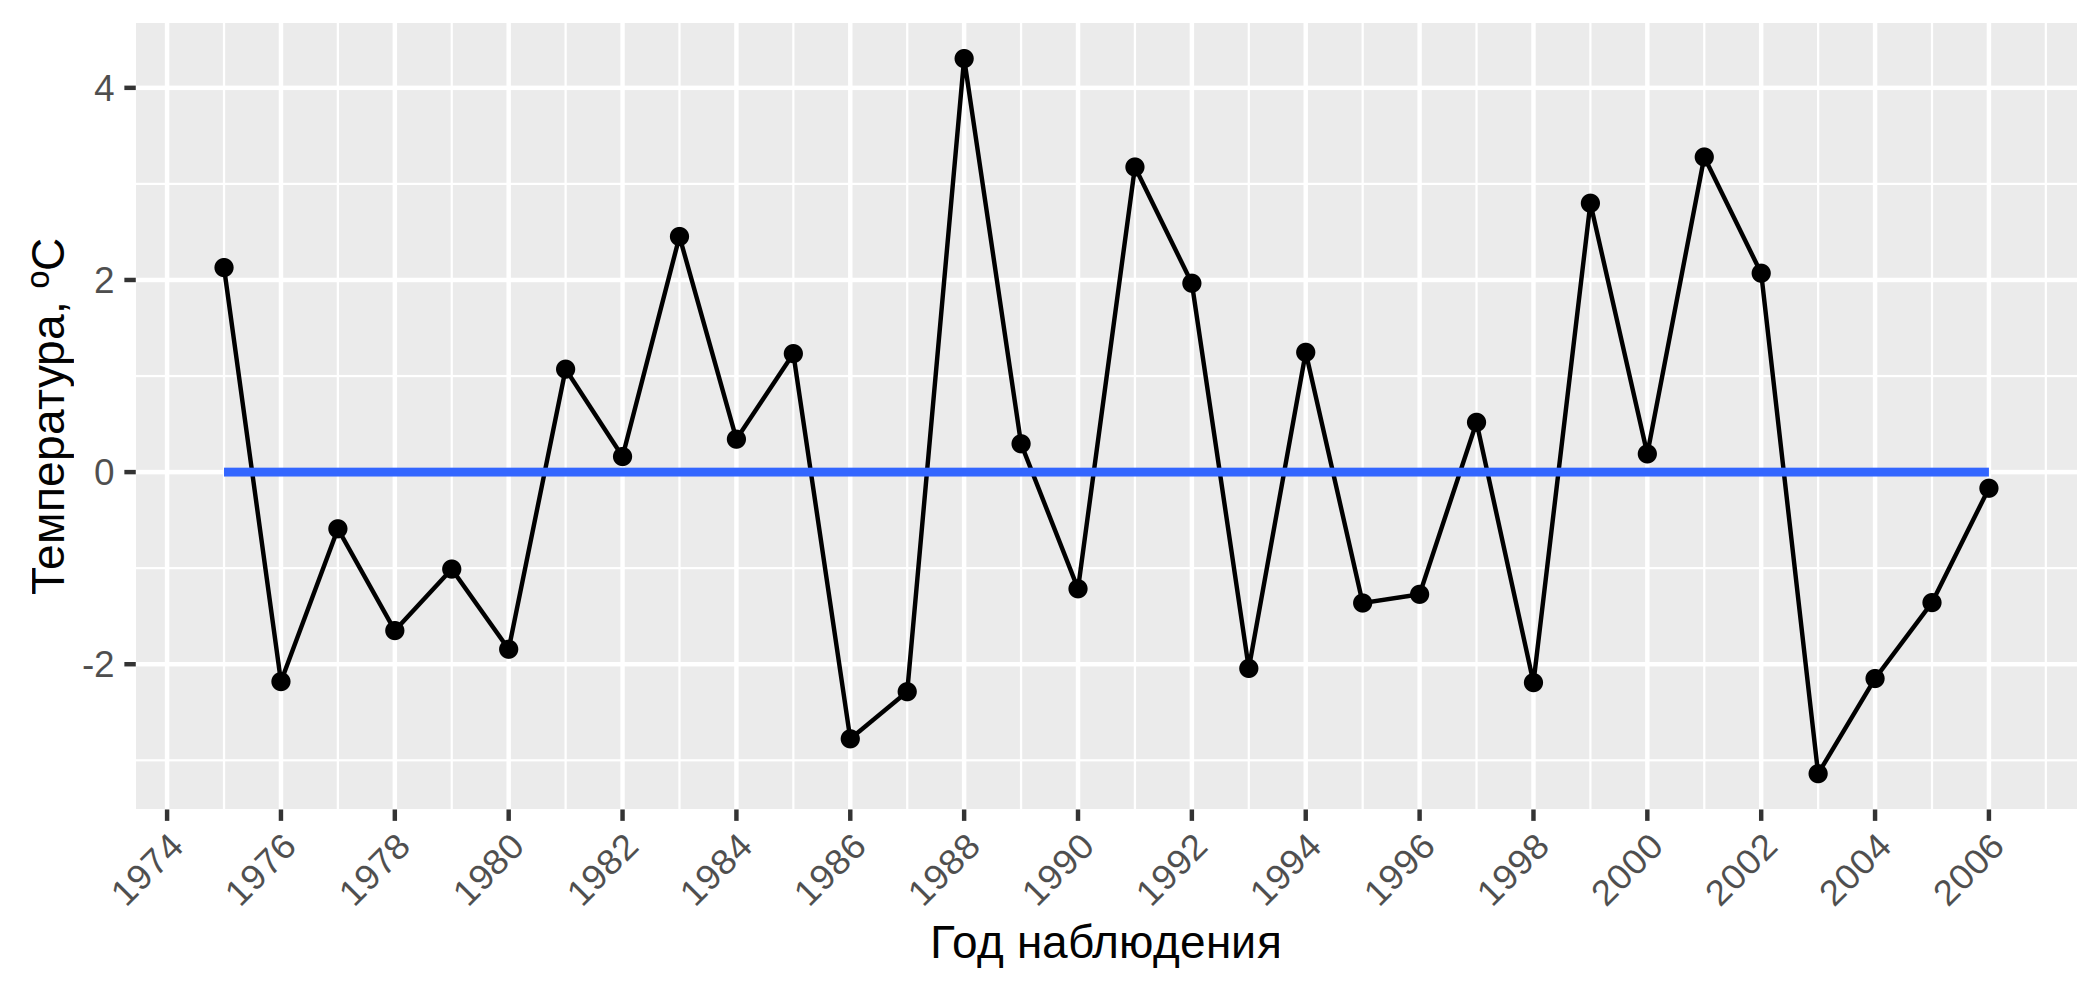
\includegraphics[width=1\linewidth]{../figures/residual/time-series.png}}
\caption{График ряда остатков}
\label{img:ts_detrended}
\end{figure}

\begin{figure}[H]
	\center{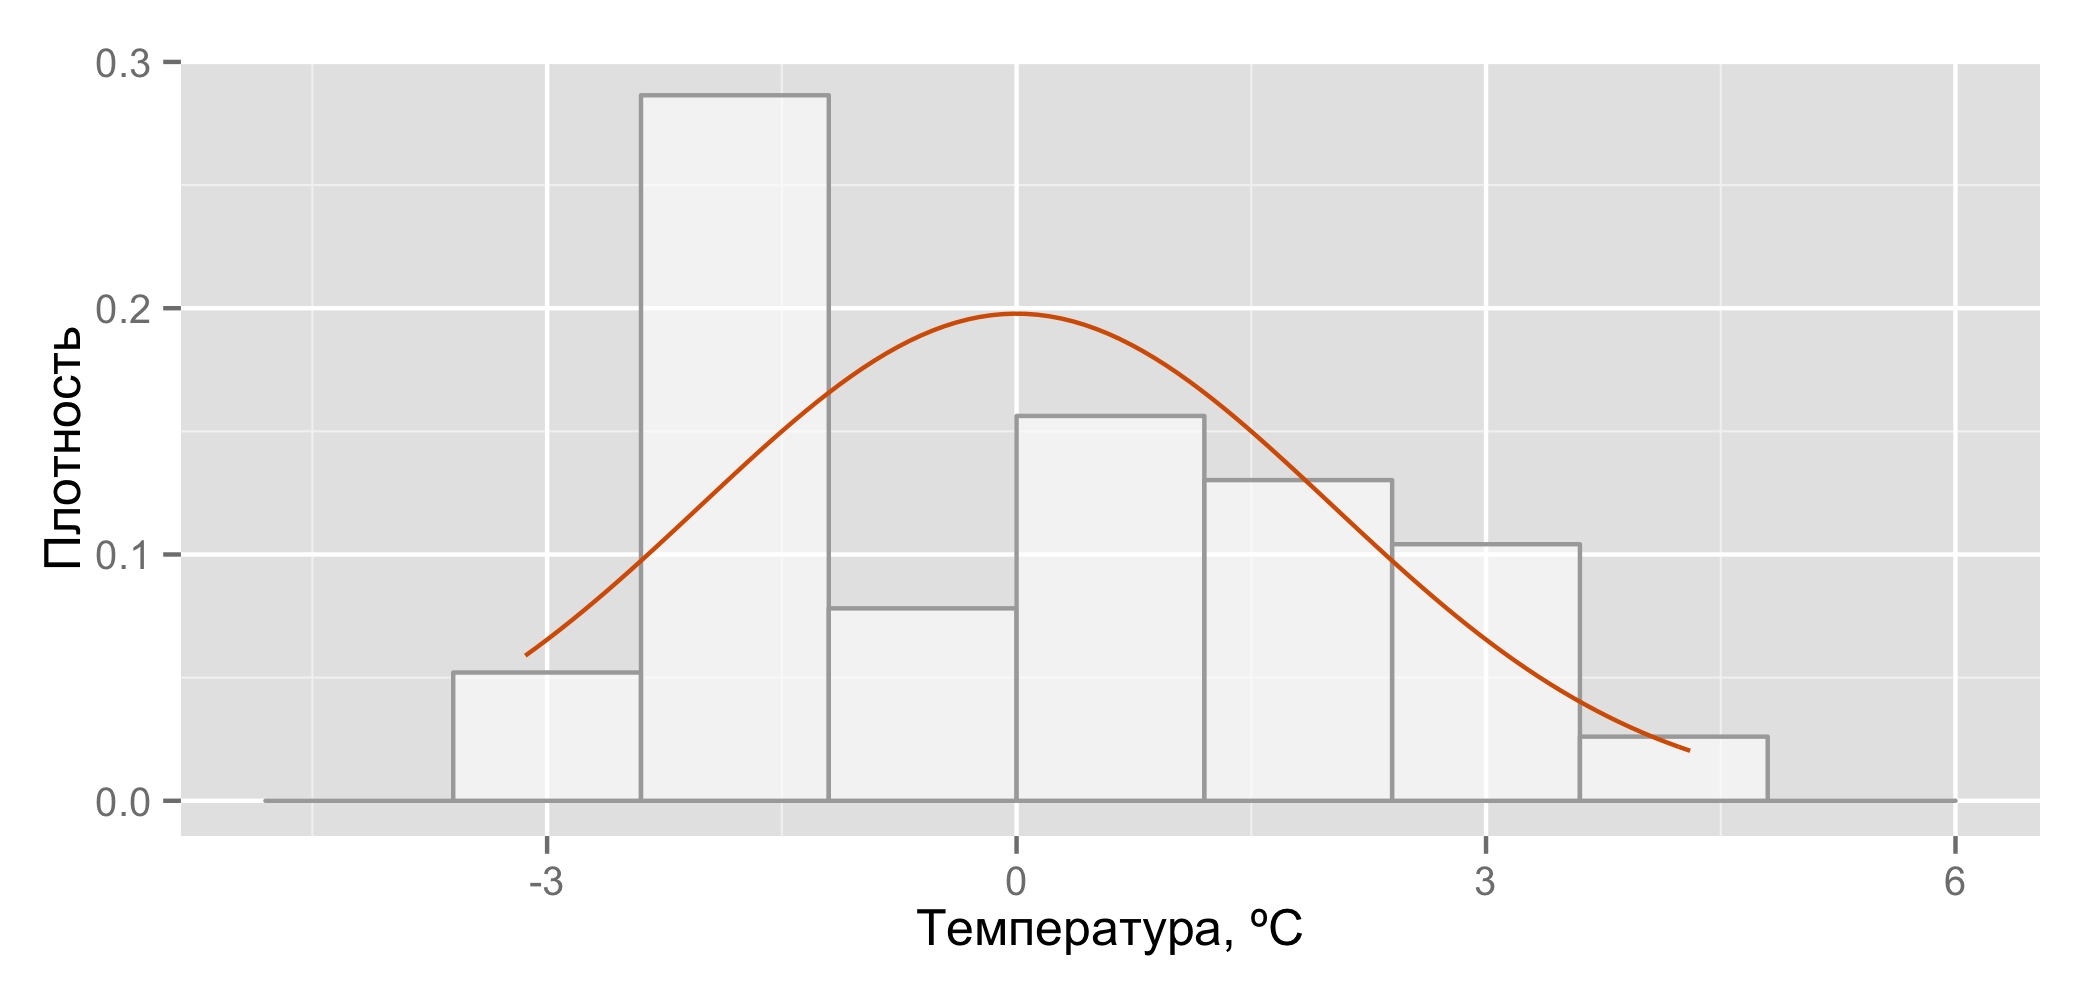
\includegraphics[width=1\linewidth]{../figures/residual/histogram.png}}
\caption{Гистограмма остатков с кривой плотности нормального распределения $\mathcal{N}(19.88, 4.92)$}
\label{img:resid_hist}
\end{figure}

\begin{figure}[H]
	\center{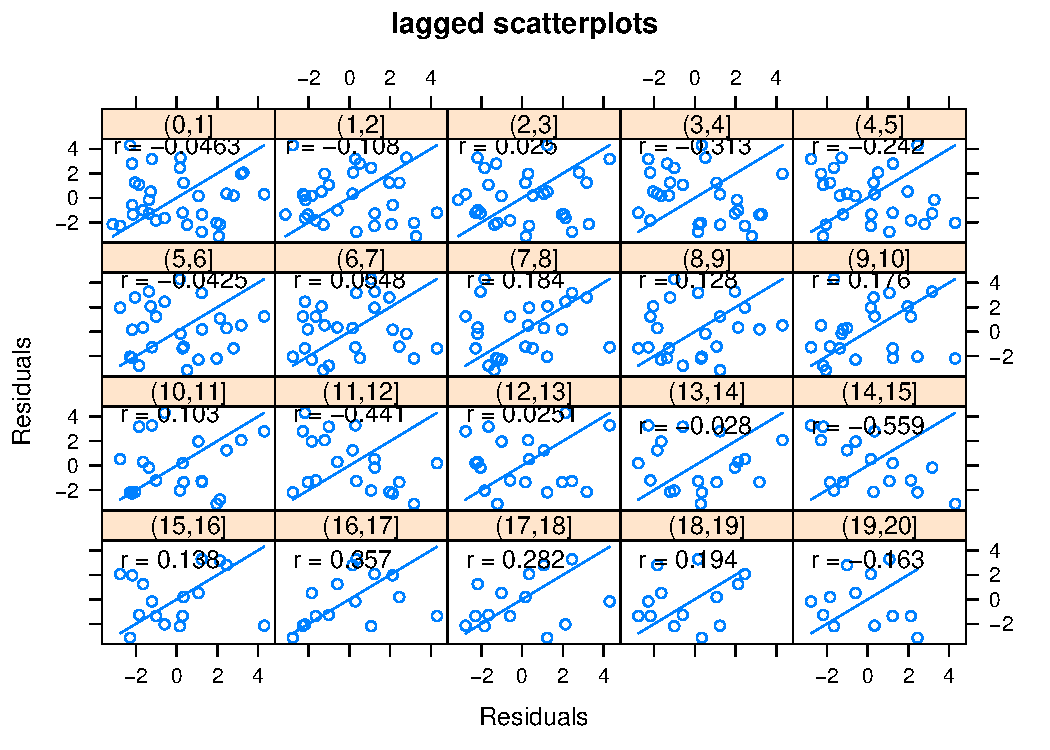
\includegraphics[width=1\linewidth]{../figures/residual/hscat.pdf}}
\caption{Диаграмма взаимного разброса}
\label{img:hscat}
\end{figure}

\begin{figure}[H]
	\center{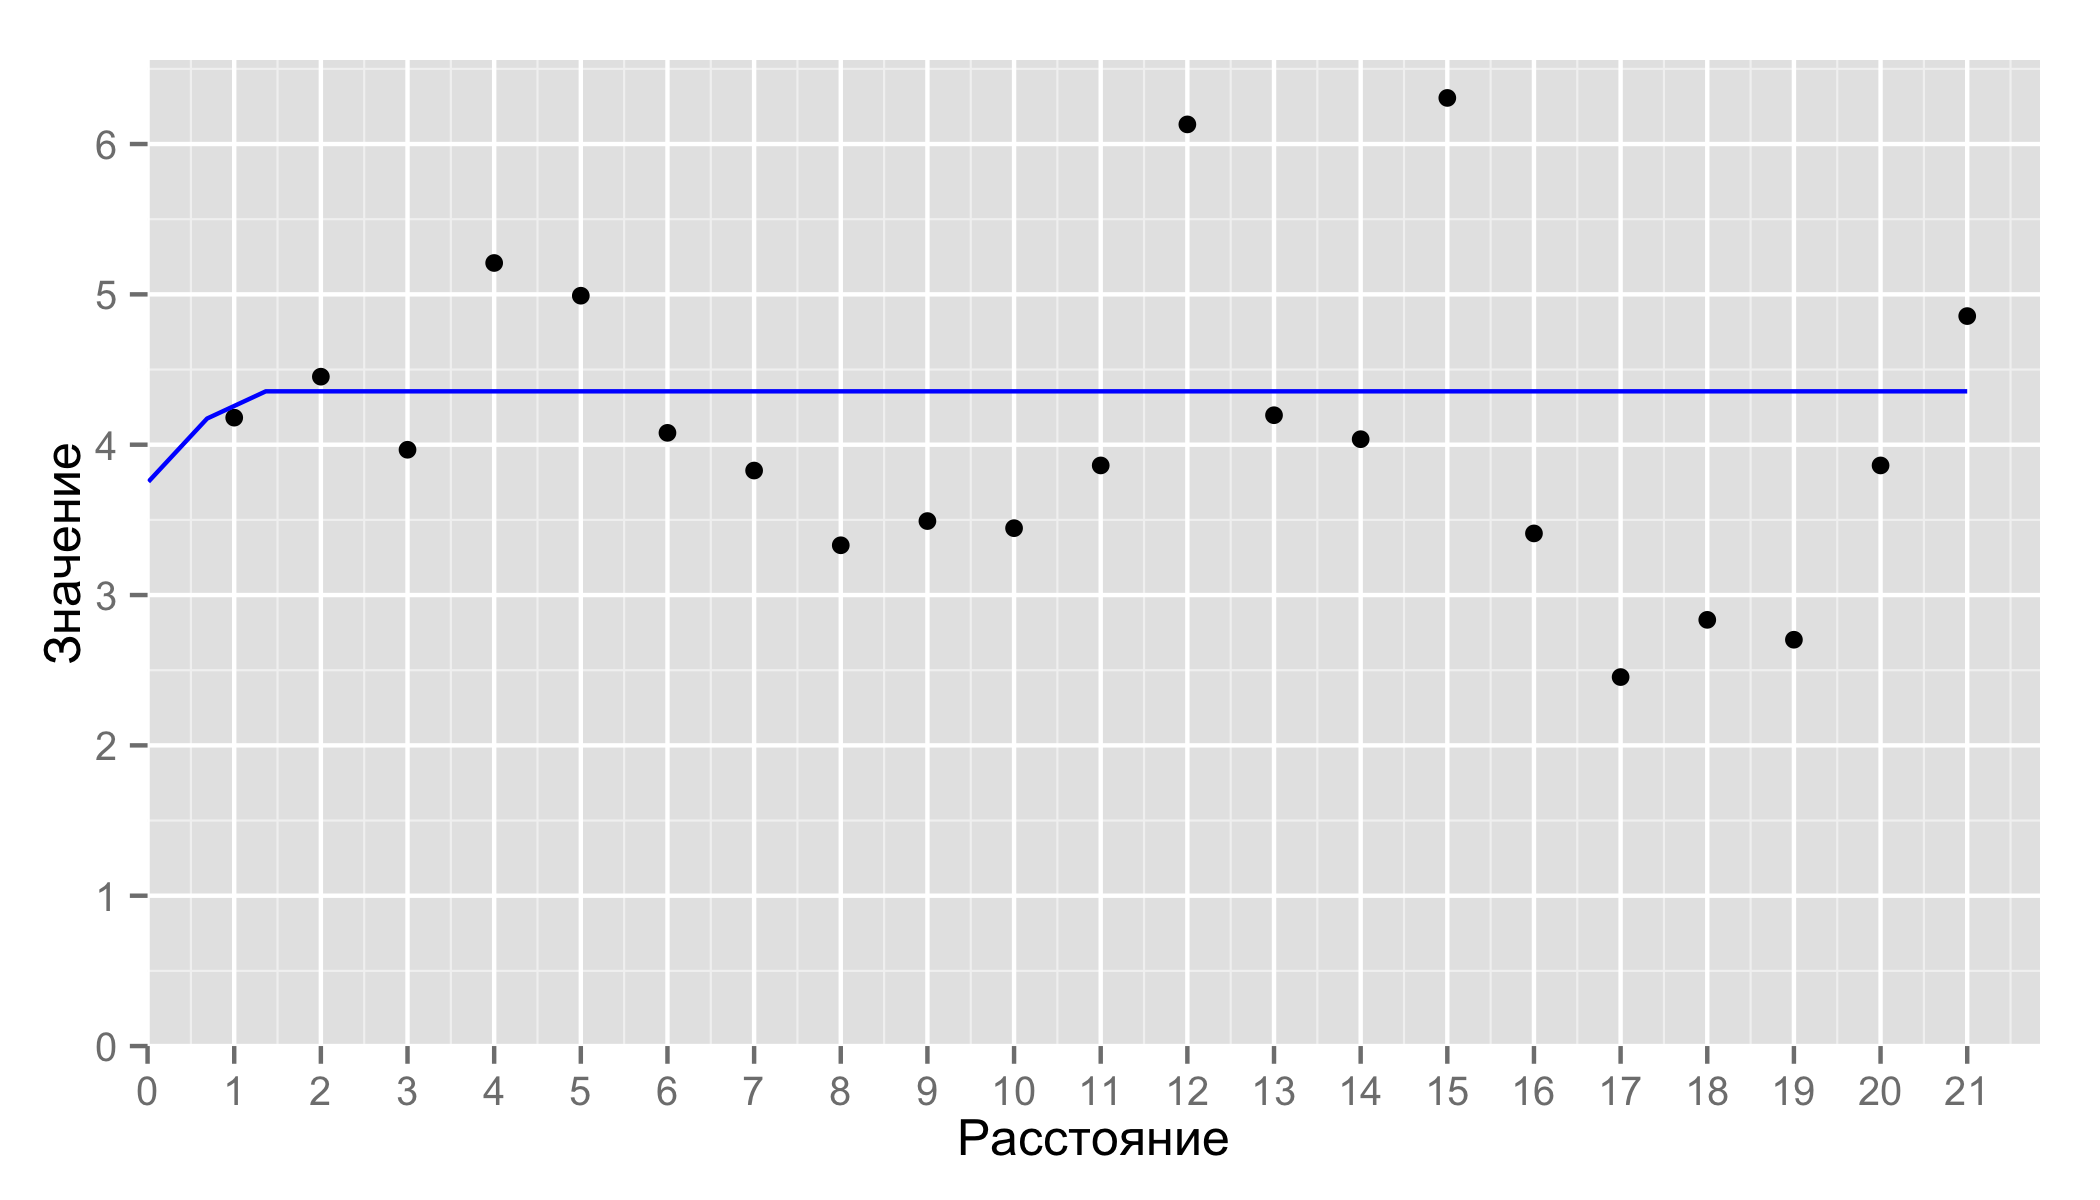
\includegraphics[width=1\linewidth]{../figures/variogram/manual-variogram.png}}
\caption{Экспериментальная и теоретическая вариограмма (сферическая модель)}
\label{img:manual-variogram}
\end{figure}

\begin{figure}[H]
	\center{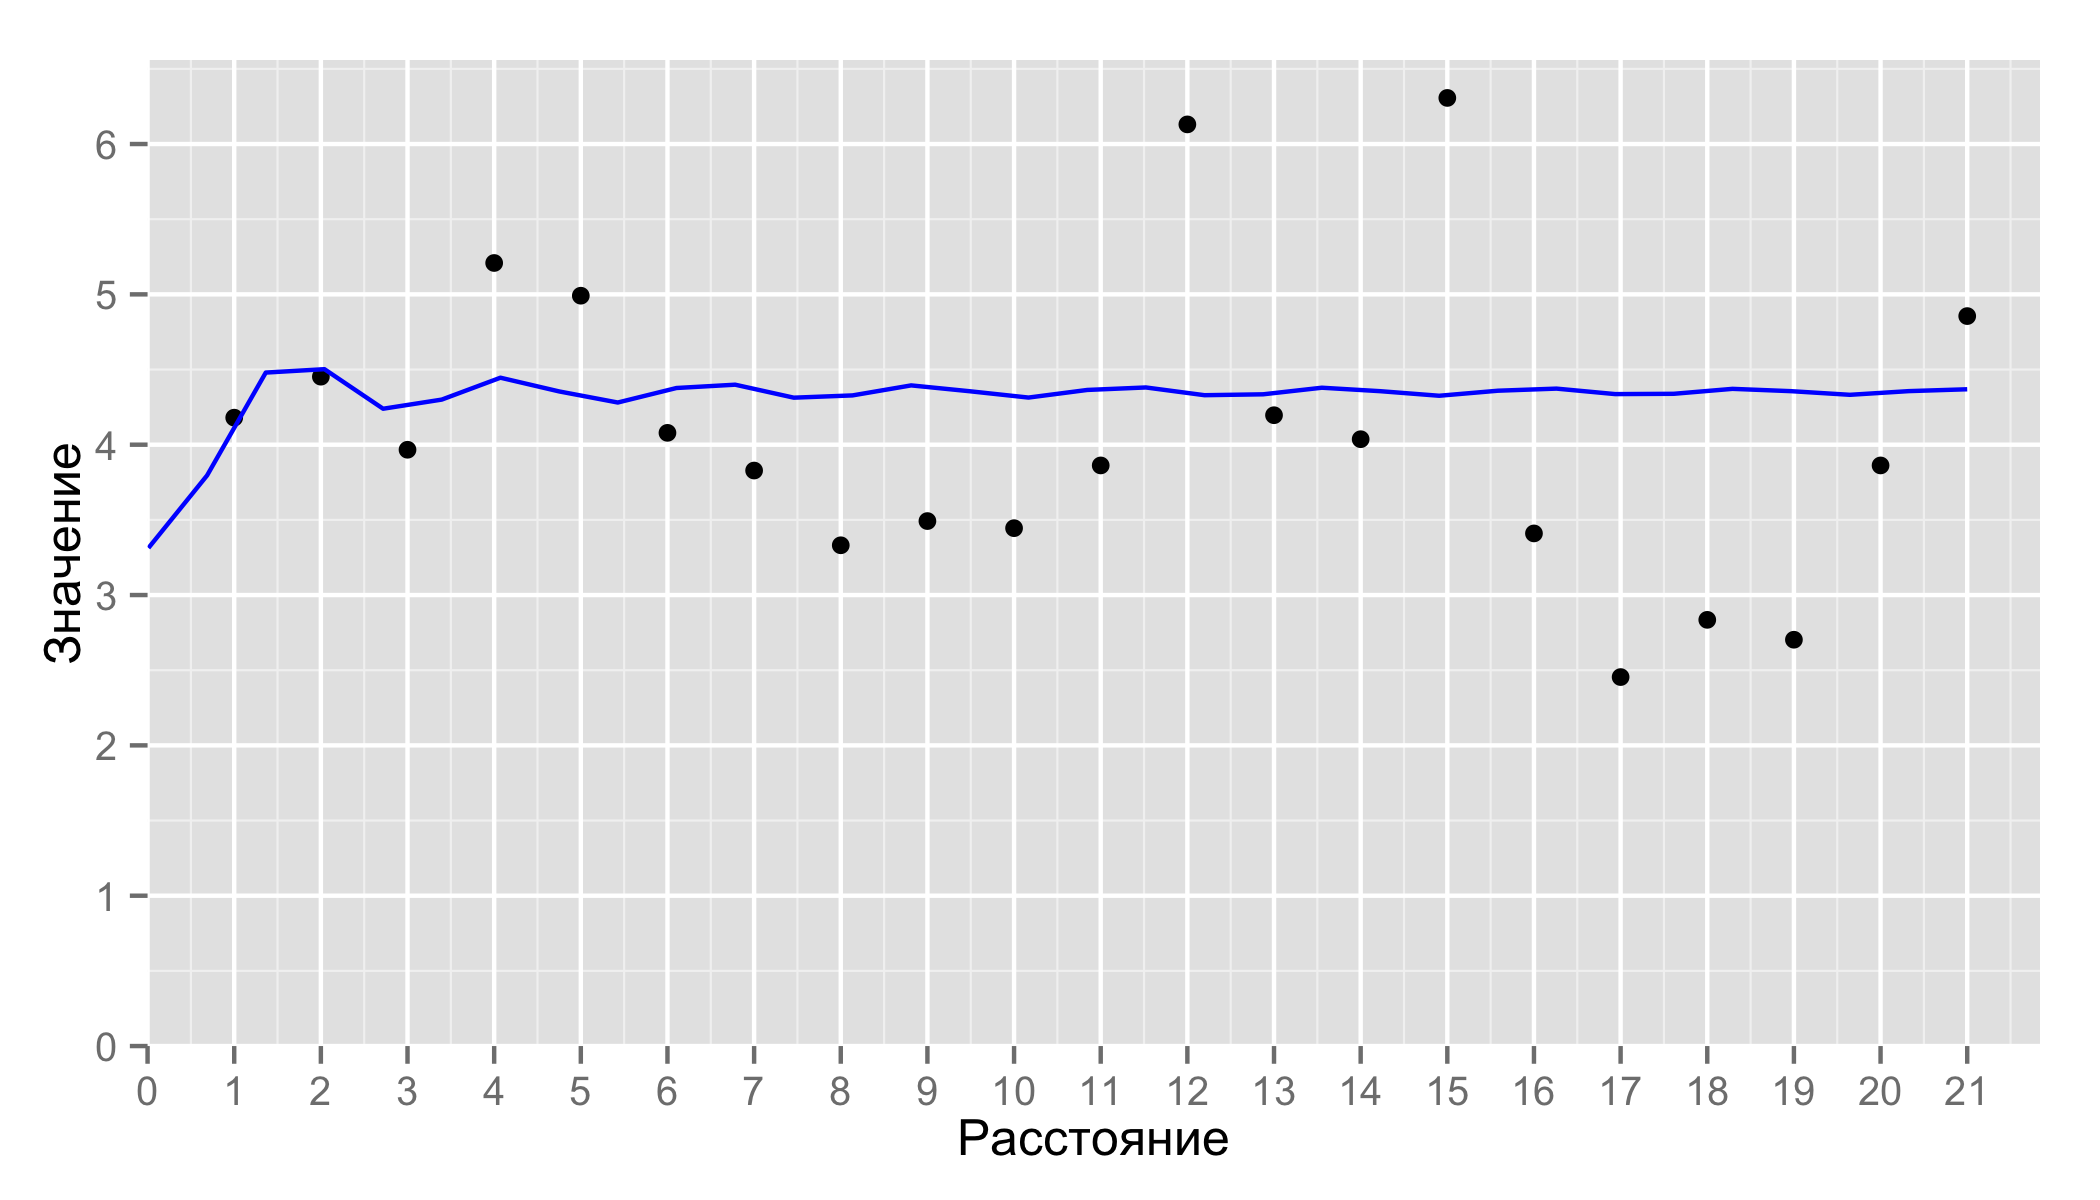
\includegraphics[width=1\linewidth]{../figures/variogram/classical-variogram.png}}
\caption{Экспериментальная и теоретическая вариограмма (классическая оценка)}
\label{img:classical-variogram}
\end{figure}

\begin{figure}[H]
	\center{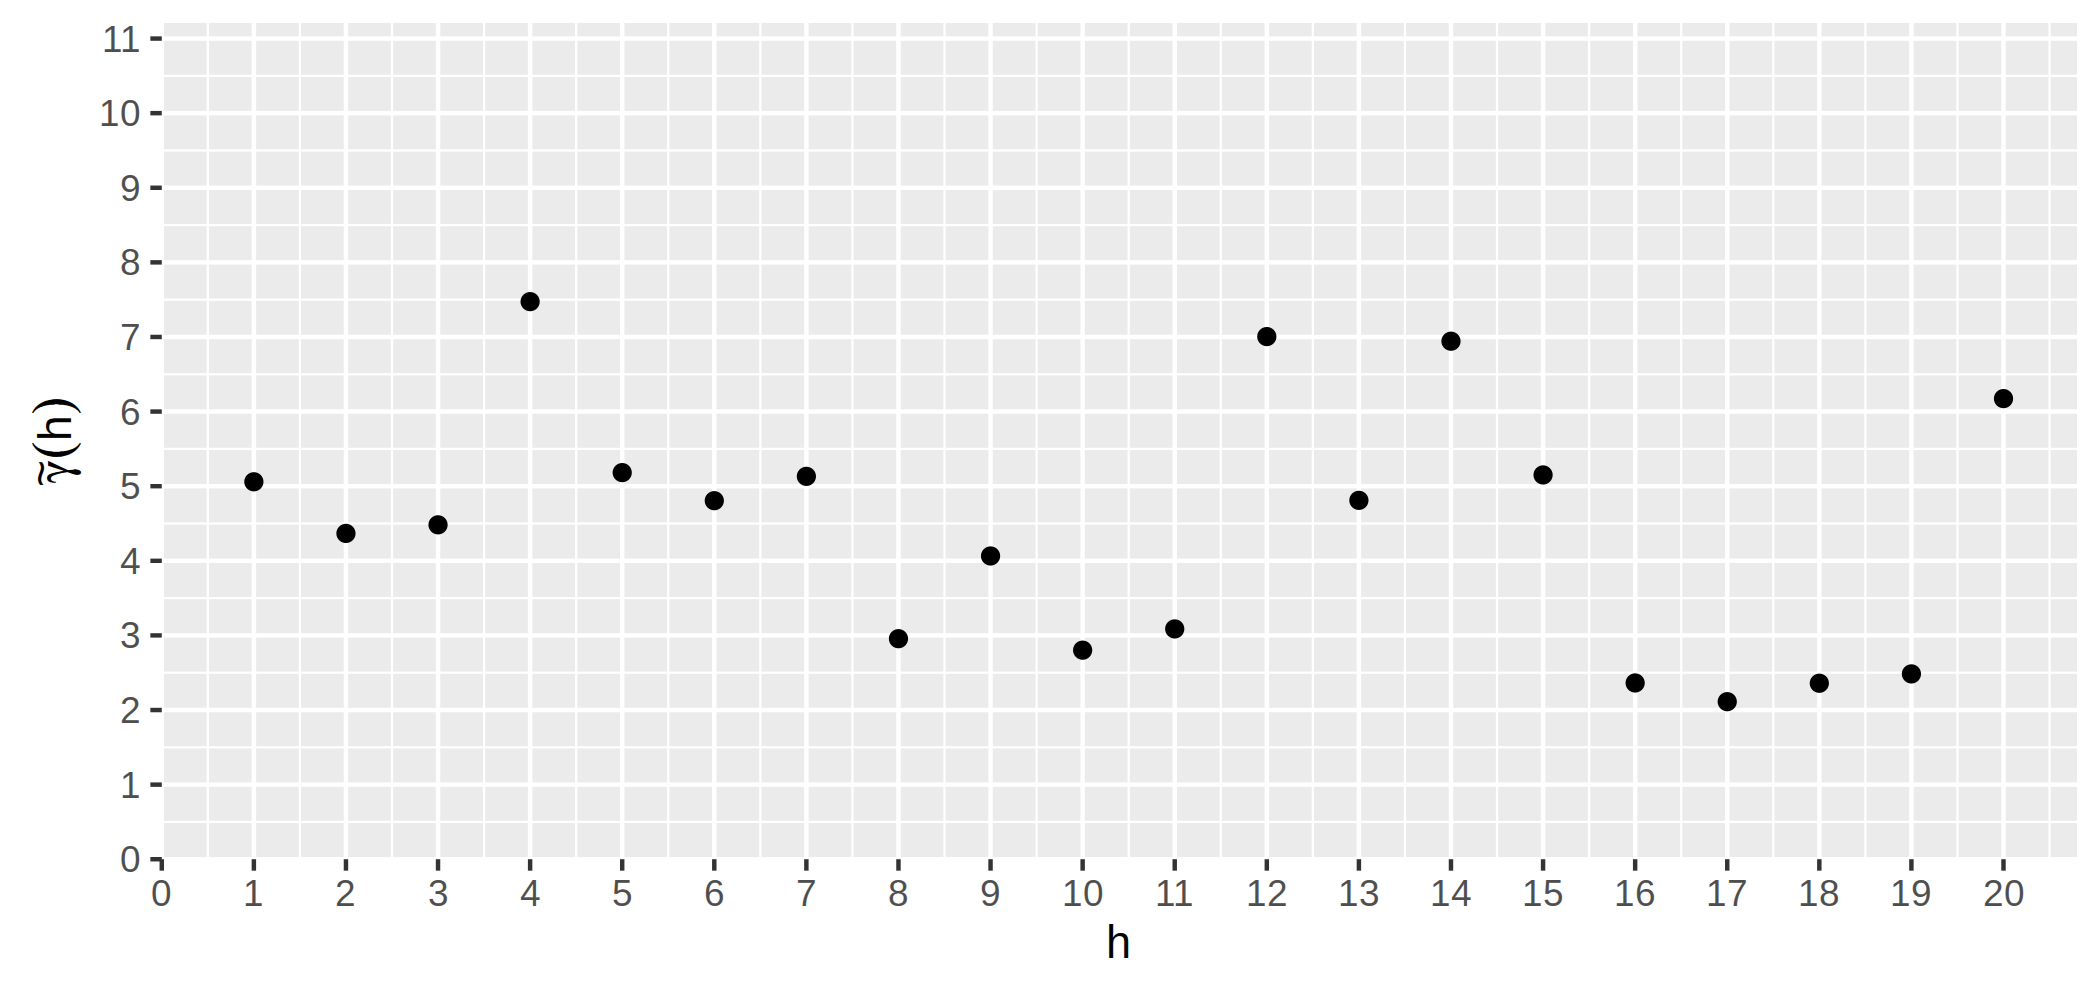
\includegraphics[width=1\linewidth]{../figures/variogram/robust-variogram.png}}
\caption{Экспериментальная и теоретическая вариограмма (робастная оценка)}
\label{img:robust-variogram}
\end{figure}

\begin{figure}[H]
\center{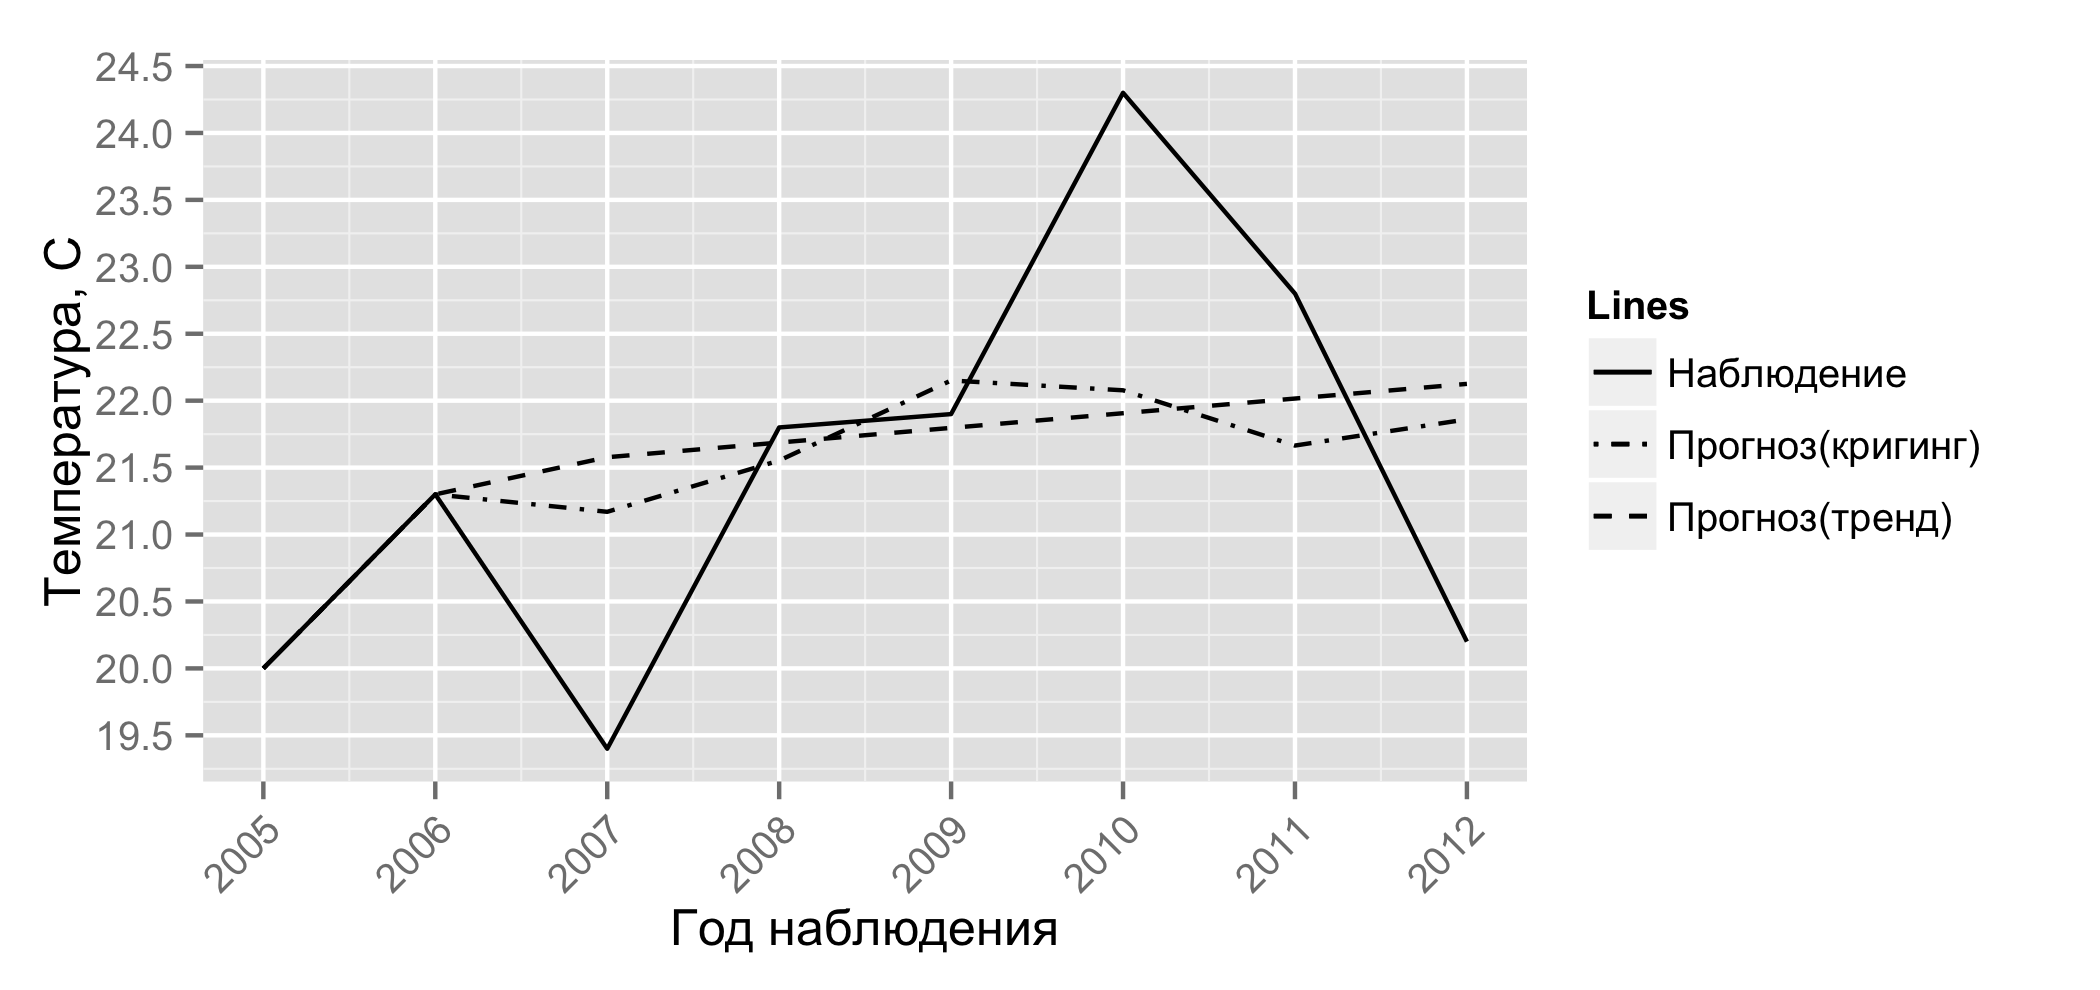
\includegraphics[width=1\linewidth]{../figures/variogram/classical-best-cross-prediction.png}}
\caption{Сравнение прогнозных значений (классическаая оценка)}
\label{img:classical-best-cross-prediction}
\end{figure}

\begin{figure}[H]
\center{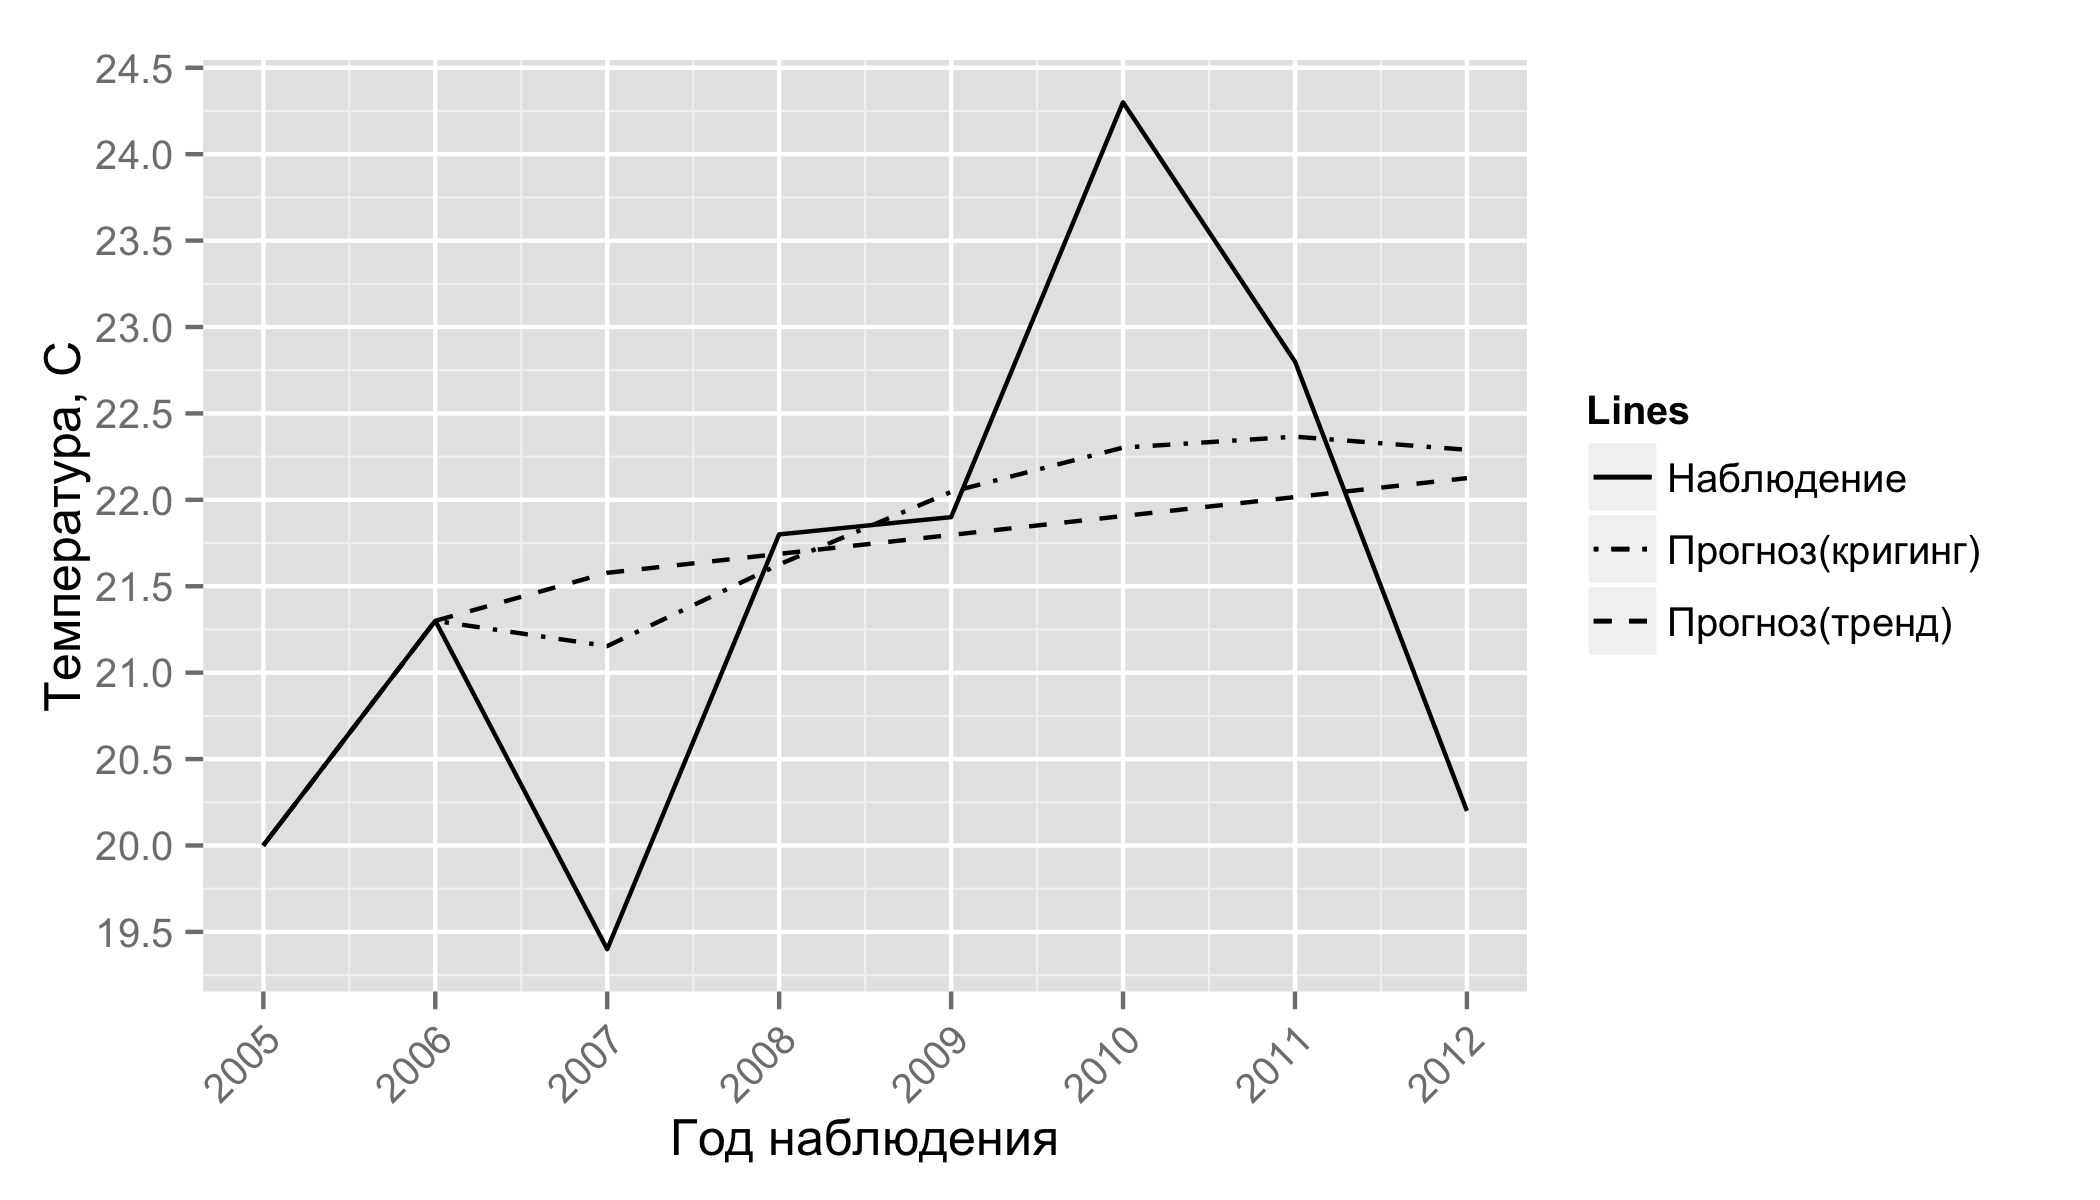
\includegraphics[width=1\linewidth]{../figures/variogram/robust-best-cross-prediction.png}}
\caption{Сравнение прогнозных значений (робастная оценка)}
\label{img:robust-best-cross-prediction}
\end{figure}

\newpage
\section{ Результаты вычислений}
\label{c:app_results}

% latex table generated in R 3.1.2 by xtable 1.7-4 package
% Fri May 15 03:15:00 2015
\begin{table}[H]
\centering
\begin{tabular}{rrr}
  \hline
 & year & temperature \\ 
  \hline
1 & 1975.00 & 2.05 \\ 
  2 & 1976.00 & -2.25 \\ 
  3 & 1977.00 & -0.66 \\ 
  4 & 1978.00 & -1.71 \\ 
  5 & 1979.00 & -1.06 \\ 
  6 & 1980.00 & -1.89 \\ 
  7 & 1981.00 & 1.04 \\ 
  8 & 1982.00 & 0.14 \\ 
  9 & 1983.00 & 2.44 \\ 
  10 & 1984.00 & 0.33 \\ 
  11 & 1985.00 & 1.23 \\ 
  12 & 1986.00 & -2.77 \\ 
  13 & 1987.00 & -2.27 \\ 
  14 & 1988.00 & 4.33 \\ 
  15 & 1989.00 & 0.33 \\ 
  16 & 1990.00 & -1.17 \\ 
  17 & 1991.00 & 3.22 \\ 
  18 & 1992.00 & 2.02 \\ 
  19 & 1993.00 & -1.98 \\ 
  20 & 1994.00 & 1.32 \\ 
  21 & 1995.00 & -1.28 \\ 
  22 & 1996.00 & -1.18 \\ 
  23 & 1997.00 & 0.62 \\ 
  24 & 1998.00 & -2.09 \\ 
  25 & 1999.00 & 2.91 \\ 
  26 & 2000.00 & 0.31 \\ 
  27 & 2001.00 & 3.41 \\ 
  28 & 2002.00 & 2.21 \\ 
  29 & 2003.00 & -2.99 \\ 
  30 & 2004.00 & -1.99 \\ 
  31 & 2005.00 & -1.20 \\ 
  32 & 2006.00 & 0.00 \\ 
  33 & 2007.00 & -2.00 \\ 
  34 & 2008.00 & 0.30 \\ 
  35 & 2009.00 & 0.30 \\ 
   \hline
\end{tabular}
\caption{Временной ряд остатков.} 
\label{table:residuals}
\end{table}

% latex table generated in R 3.1.3 by xtable 1.7-4 package
% Tue May 19 03:07:10 2015
\begin{table}[ht]
\centering
\begin{tabular}{rrrrr}
  \hline
 & Год & Наблюдение & Прогноз & Тренд \\ 
  \hline
1 & 2007 & 19.400 & 21.577 & 21.578 \\ 
  2 & 2008 & 21.800 & 21.688 & 21.687 \\ 
  3 & 2009 & 21.900 & 21.798 & 21.797 \\ 
  4 & 2010 & 24.300 & 21.907 & 21.906 \\ 
  5 & 2011 & 22.800 & 22.017 & 22.016 \\ 
  6 & 2012 & 20.200 & 22.126 & 22.126 \\ 
   \hline
\end{tabular}
\caption{Прогноз (сферическая модель)} 
\label{table:manual-prediction}
\end{table}


\newpage
\section{ Код программ}
\label{c:listings}
\renewcommand{\thelstlisting}{D.1}
\lstinputlisting[language=R, caption=Описательные статистики, label=lst:dstats]{../R/lib/dstats.R}
\renewcommand{\thelstlisting}{D.2}
\lstinputlisting[language=R, caption=Основной код программы, label=lst:main]{../R/master.R}
\renewcommand{\thelstlisting}{D.3}
\lstinputlisting[language=R, caption=Вариограммный анализ, label=lst:variogram]{../R/predictor.R}

  \bibliographystyle{unsrt}
\bibliography{bibliography/bibdb}

\end{document}